\documentclass[a4paper]{article}
\usepackage[german,english]{babel}
\usepackage{amsmath}
\usepackage{amssymb}
\usepackage{amsthm}
\usepackage{graphicx}
\usepackage{caption}
\usepackage{fontspec}
\usepackage{mdframed}
\usepackage{pxfonts}
\usepackage{wasysym}
\usepackage{framed}
\usepackage{xcolor}
\usepackage{makeidx}
\usepackage{csquotes}
\usepackage[pdfborder={0 0 0}]{hyperref}
\usepackage{stmaryrd}
\usepackage{unicode-math}
\usepackage{titlesec}
\titleformat{\paragraph}{\normalfont\itshape}{}{}{}

% okay-ish main typefaces: Alegreya, Junicode, CMU Concrete, Linux Libertine O, Libertinus Serif, URW Palladio L, Bookerly, Andada
\setmainfont{Alegreya}
\setmathfont{cmr10}


\newcounter{lecref}[section]
\numberwithin{lecref}{section}

\theoremstyle{break}
\newmdtheoremenv[
    linecolor=white,%
    backgroundcolor=gray!10,%
    innertopmargin=0pt]{theorem}{Theorem}[lecref]

\newtheorem{thm}[lecref]{Theorem}
\newtheorem*{Thm}{Theorem}
\newtheorem{example}[lecref]{Example}
\newtheorem*{Example}{Example}
\newtheorem{definition}[lecref]{Definition}
\newtheorem*{Definition}{Definition}
\newtheorem{lemma}[lecref]{Lemma}
\newtheorem*{Lemma}{Lemma}
\newtheorem{claim}[lecref]{Claim}
\newtheorem*{Claim}{Claim}
\newtheorem{remark}[lecref]{Remark}
\newtheorem*{Remark}{Remark}
\newtheorem{algorithm}{Algorithm}
\newtheorem*{Algorithm}{Algorithm}
\newtheorem{corollary}[lecref]{Corollary}
\newtheorem*{Corollary}{Corollary}
\newtheorem{proposition}[lecref]{Proposition}
\newtheorem*{Proposition}{Proposition}


\def\ifempty#1{\def\temp{#1} \ifx\temp\empty }

% chronological structure of lectures
\newcommand{\dateref}[1]{%
  \begin{mdframed}[backgroundcolor=gray!10,innerbottommargin=0pt,innertopmargin=0pt]
    \paragraph{\textit{$\downarrow$ This lecture took place on #1.}}%
  \end{mdframed}%
}

% useful control sequences for mathematical notation
\newcommand{\Abs}[1]{\left|#1\right|}
\newcommand{\Set}[1]{\left\{#1\right\}}
\newcommand{\SetDef}[2]{\left\{#1\,\mid\,#2\right\}}
\newcommand{\IP}[2]{\left\langle#1, #2\right\rangle}
\newcommand{\Norm}[1]{\left\|{\ifempty{#1}\cdot\else#1\fi}\right\|}
\newcommand{\Max}[1]{\max{\Set{#1}}}
\newcommand{\Min}[1]{\min{\Set{#1}}}
\newcommand{\Sup}[1]{\sup{\Set{#1}}}
\newcommand{\Powerset}[1]{{\mathbb P}(#1)}
\newcommand{\IntRange}[2]{#1, \dots\ifempty{#2}\else, #2\fi}

\def\vec2#1#2{\begin{pmatrix} #1 \\ #2 \end{pmatrix}}
\def\vec3#1#2#3{\begin{pmatrix} #1 \\ #2 \\ #3 \end{pmatrix}}
\newcommand{\noproof}[1]{A proof for Theorem~\ref{#1} is not provided.}
\newcommand{\dotted}[1]{\:\dot{#1}\:}  % dot has too little margin

% German translation
\newcommand{\dt}[1]{(dt. \enquote{\foreignlanguage{german}{#1}})}

% essential control sequences
%% \xRightarrow: \xrightarrow for \rightarrow like \xRightarrow for \Rightarrow
\makeatletter
\newcommand{\xRightarrow}[2][]{\ext@arrow 0359\Rightarrowfill@{#1}{#2}}
\makeatother

% typesetting settings
\parindent0pt
\setlength{\parskip}{.6em}

% TODO: span?
\DeclareMathOperator{\rank}{rank}
\DeclareMathOperator{\diag}{diag}
\DeclareMathOperator{\detm}{det}
\DeclareMathOperator{\perm}{perm}
\DeclareMathOperator{\sign}{sign}
\DeclareMathOperator{\degree}{deg}
\DeclareMathOperator{\im}{image}
\DeclareMathOperator{\ke}{kernel}
\DeclareMathOperator{\spec}{spec}
\DeclareMathOperator{\prop}{probability}
\DeclareMathOperator{\Hom}{Hom}
\DeclareMathOperator{\argmax}{argmax}
\DeclareMathOperator{\argmin}{argmin}
\DeclareMathOperator{\vol}{vol}  % volume
\DeclareMathOperator*{\bigtimes}{\vartimes}

% https://tex.stackexchange.com/a/110981, CC BY-SA
\makeatletter
\providecommand*{\dotcup}{%
  \mathbin{%
    \mathpalette\@dotcup{}%
  }%
}
\newcommand*{\@dotcup}[2]{%
  \ooalign{%
    $\m@th#1\cup$\cr
    \hidewidth$\m@th#1\cdot$\hidewidth
  }%
}
\makeatother

% metadata
\title{
  Computational Mathematics 1 \\
  \large{Lecture notes, University (of Technology) Graz} \\
  based on the lecture by Tobias Breiten
}
\date{\today}
\author{Lukas Prokop}

% generate index database
\makeindex

\begin{document}

\maketitle
\tableofcontents

\section*{Course}

\dateref{2018/10/02}

\begin{itemize}
  \item \href{https://imsc.uni-graz.at/breiten/teaching/numa18/}{Homepage at uni-graz.at}
  \item Contents:
    \begin{enumerate}
      \item Linear equation system
      \item Numerical error analysis
      \item Curve fitting~\dt{Lineare Ausgleichsrechnung}
      \item Non-linear equations
      \item Interpolation
      \item Numerical integration
    \end{enumerate}
  \item Literature:
    \begin{enumerate}
      \item Deuflhard, Hohmann: Numerische Mathematik 1
      \item Schwarz, Köckler: Numerische Mathematik
    \end{enumerate}
\end{itemize}

\clearpage
\section{What is Computational Mathematics?}
%
Computational Mathematics as branch of mathematics considers the construction and analysis of algorithms for continuous mathematical problems.
More specifically, based on a model and input data, we construct specific output data of interest.
Formally, we associate a model using function $f: X \to Y$ where $X$ is the set of input data and $Y$ the set of output data. The problem is to find output $f(x) \in Y$ for given $x \in X$.

Examples:
\begin{itemize}
  \item Addition of two numbers: $X = \mathbb R^2, Y = \mathbb R, f: (x_1, x_2) \mapsto x_1 + x_2$
  \item Solution of a linear equation system: $Ax = b$
    \[ X = \mathbb R^{n \times n} \times \mathbb R^n, Y = \mathbb R^n, f: (A, b) \mapsto A^{-1} b \]
\end{itemize}

An algorithm is defined as unambiguous sequence of steps to solve a given problem. A problem is characterized as
\begin{itemize}
  \item the input data required for computation
  \item the output data that represent the solution of the algorithm
  \item the description of the steps to be done, including auxiliary values
\end{itemize}
We require, the algorithm is
\begin{description}
  \item[executable] by a machine
  \item[terminating] after a finite number of steps
  \item[deterministic] as the same input always leads to the same output
\end{description}
Furthermore we analyze the algorithm in terms of
\begin{description}
  \item[stability] small errors in the input lead to small errors in the output
  \item[precision] output data should solve the problem with maximum accuracy
  \item[efficiency] large problems can be solved in practical time
\end{description}

Consider the linear equation system
\begin{align*}
  a_{11} x_1 + a_{12} x_2 + \dots + a_{1n} x_n &= b \\
  \vdots &= \vdots \\
  a_{n1} x_1 + a_{n2} x_2 + \dots + a_{nn} x_n &= b \\
\end{align*}
The same can be specified in compact notation like $Ax = b$ with $A \in \mathbb R^{n \times n}, b \in \mathbb R^n$.

\index{Cramer's rule}
\begin{thm}[Cramer's Rule]
  Let $A \in \mathbb R^{n \times n}$ with $\det(A) \neq 0$ and $b \in \mathbb R^n$.
  Then there exists exactly one $x \in \mathbb R^n$ such that $Ax = b$. We can determine $x$ using \enquote{Cramer's Rule}:
  \[
    x_i = \frac{\det(A_i)}{\det(A)} \text{ where }
    A_i = \begin{bmatrix}
      a_{11} & \dots & a_{1, i-1} & b_1 & a_{1,i+1} & \dots & a_{1n} \\
      \vdots &       &            &     &           &       & \vdots \\
      a_{n1} & \dots & a_{n,i-1}  & b_n & a_{n,i+1} & \dots & a_{nn}
    \end{bmatrix}
  \]
\end{thm}

\begin{Remark}[Problem]
  Computation using $\det(A) = \sum_{\sigma \in S_n} \sign(\sigma) a_{1,\sigma(1)} \dots a_{n,\sigma(n)}$ requires $n \cdot n!$ operations.
\end{Remark}

\subsection{Solving linear eq. system by forward/backwards substitution}
%
Consider the special case of a linear equation system of structure
\[
  \begin{array}{rrrrl}
    \gamma_{11} x_1 &+ \gamma_{12} x_2 &+ \dots &+ \gamma_{1n} x_n &= z_1 \\
                    &  \gamma_{22} x_2 &+ \dots &+ \gamma_{2n} x_n &= z_2 \\
                    &                  & \ddots &                  &= \vdots \\
                    &                  &        &  \gamma_{nn} x_n &= z_n
  \end{array}
\]%
\index{Backwards substitution}%
and accordingly, $Rx = z$ with an upper triangular matrix, hence $\gamma_{ij} = 0$ for $i > j$.
We retrieve $x$ by recursive solution (by so-called \enquote{backwards substitution}) starting with row $n$:
\begin{align*}
  x_n &= \frac{z_n}{\gamma_{nn}} \text{ if } \gamma_{nn} \neq 0 \\
  x_{n-1} &= \frac{z_{n-1} - \gamma_{n-1,n} x_n}{\gamma_{n-1,n-1}} &\text{ if } \gamma_{n-1,n-1} \neq 0 \\
  x_{1} &= \frac{z_1 - \gamma_{12} x_2 - \dots - \gamma_{1n} x_n}{\gamma_{11}} &\text{ if } \gamma_{11} \neq 0
\end{align*}

Obviously, it holds that
\[ \det(R) = \gamma_{11} \dots \gamma_{nn} \neq 0 \iff \gamma_{ii} \neq 0 \qquad \forall i = 1, \dots, n \]
The algorithm is applicable (just like Cramer's rule), if $\det(R) \neq 0$.
Then the existence of a solution is guaranteed and this solution is unique.

\begin{Remark}[Computing time]\hfill{}
  \begin{enumerate}
    \item for the $i$-th row, we need $(n-i)$ additions, $(n-i)$ multiplications and one division
    \item in total for the rows $n$ to $1$,
      \[ \sum_{i=1}^n (i - 1) = \frac{n (n - 1)}2 \dotted{=} \frac{n^2}2 \]
      Multiplication and the same amount of additions.
      The notation $\dot=$ is used to denote equivalence up to terms of same degree.
      Analogously, the equation system $Lx = z$ can be solved with a lower triangular matrix $L$ by forward substitution starting with the first row.
  \end{enumerate}
\end{Remark}

\subsection{Gaussian elimination process}
\label{sec:1-2}

\emph{Basic idea:}
\begin{quote}
  Beginning with a linear equation system of structure,
  \begin{align}
    a_{11} x_1 + a_{12} x_2 + \dots + a_{1n} x_n &= b_1 \nonumber\\
    a_{21} x_1 + a_{22} x_2 + \dots + a_{2n} x_n &= b_2 \nonumber\\
    \vdots &= \vdots \nonumber\\
    a_{n1} x_1 + a_{n2} x_2 + \dots + a_{nn} x_n &= b_n
    \label{eq1}
  \end{align}
  we apply equivalence transformations to end up with an upper triangular matrix.
\end{quote}

As a first step, we eliminate variable $x_1$ of rows $2$ to $n$.
\begin{align}
  a_{11} x_1 + a_{12} x_2 + \dots + a_{1n} x_n &= b_1 \nonumber\\
    a_{22}' x_2 + \dots + a_{2n}' x_n &= b_1 \nonumber\\
      \vdots &= \vdots \nonumber\\
      a_{12}' x_2 + \dots + a_{nn}' x_n &= b_n'
  \label{eq2}
\end{align}
So we apply this elimination step ($r_i \coloneqq \frac{r_i}{a_{i1}} - \frac{r_1}{a_{11}}$ where $r_i$ denotes the $i$-th row) to the last $n-1$ rows and determine the triangular matrix recursively this way.

Consider the transformation of~\eqref{eq1} to \eqref{eq2}.
Let $a_{11} \neq 0$ and we recognize $\text{row}_i \coloneqq \text{row}_i - l_{i_1} \cdot \text{row}_1$.
Formally,
\[ \underbrace{(a_{i1} - l_{i1} a_{11}) x_1}_{=0} + \underbrace{(a_{i2} - l_{i1} a_{12})}_{a_{i2}'} x_2 + \dots + \underbrace{(a_{in} - l_{i1} a_{1n})}_{a_{in}'} x_n = \underbrace{b_i - l_{in} b_1}_{b_i'} \]
\[ \implies l_{in} = \frac{a_{i1}}{a_{11}} \]
hence, the first elimination step is applicable if $a_{11} \neq 0$ is given.
If we apply this step, we retrieve a sequence of matrices:
\[ A = A^{(1)} \to A^{(2)} \to \dots \to A^{(n)} = R \]
where
\[
  A^{(k)} = \begin{bmatrix}
    a_{11}^{(1)} & a_{12}^{(1)} & \dots  &              &        & a_{1n}^{(1)} \\
    0            & a_{22}^{(2)} & \dots  &              &        & a_{2n}^{(2)} \\
                 &              & \ddots &              &        & \vdots \\
                 &              &        & a_{kk}^{(k)} & \dots  & a_{kn}^{(k)} \\
                 &              &        & \vdots       &        & \vdots \\
                 &              &        & a_{nk}^{(k)} & \dots  & a_{nn}^{(k)}
  \end{bmatrix}
\]
with a remaining matrix of dimension $(n - k + 1) \times (n - k + 1)$.
For every remaining matrix we can apply the elimination step
\begin{align*}
  l_{ik} &= \frac{a_{ik}^{(k)}}{a_{kk}^{(k)}} &\text{ for } i = k+1, \dots, n \\
  a_{ij}^{(k+1)} &= a_{ij}^{(k)} - l_{ik} a_{kj}^{(k)} &\text{ for } i,j = k+1, \dots, n \\
  b_i^{(k+1)} &= b_i^{(k)} - l_{ik} b_k^{(k)} &\text{ for } i = k+1, \dots, n
\end{align*}
under the assumption that $a_{kk}^{(k)} \neq 0$ (pivot element).

\index{Frobenius matrix}
\begin{Remark}
  Every elimination step is a linear operation of the rows of $A$.
  Hence it is representable by left multiplication with $L_k \in \mathbb R^{n \times n}$ according to $A^{k+1} = L_k A^{(k)}$ and $b^{(k+1)} = L_k b^{(k)}$.

  The following matrix is a \emph{Frobenius matrix}, which has an interesting property regarding its inverse:
  \index{Frobenius matrix}
  \[
    L_k = \begin{pmatrix}
      1 &        &   &                 &        & \\
        & \ddots &   &                 &        & \\ 
        &        & 1 &                 &        & \\
        &        & -l_{k+1,k} & \ddots &        & \\
        &        & \vdots     &        & \ddots & \\
        &        & -l_{n,k}   & \dots  &        & 1
    \end{pmatrix}
    \iff
    L_k^{-1} = \begin{pmatrix}
      1 &        &   &                 &        & \\
        & \ddots &   &                 &        & \\ 
        &        & 1 &                 &        & \\
        &        & l_{k+1,k}  & \ddots &        & \\
        &        & \vdots     &        & \ddots & \\
        &        & l_{n,k}    & \dots  &        & 1
    \end{pmatrix}
  \]
\end{Remark}
and
\[
  L = L_1^{-1} \quad \dots \quad L_{n-1}^{-1} =
  \begin{pmatrix}
    1      &        &        &           & 0 \\
    l_{21} & \ddots &        &           & \\
    l_{31} & l_{32} & \ddots &           & \\
    \vdots & \vdots &        &           & \\
    l_{n1} & \dots  &        & l_{n,n-1} & 1
  \end{pmatrix}
\] \[
  L^{-1} = L_{n-1} \dots L_1
\]

\index{LR decomposition}
This way, we retrieve an equivalent linear equation system to $Rx = z, R = L^{-1} A, z = L^{-1} b$.
The representation $A = LR$ is called \emph{LR decomposition of $A$}.
If they exists, $L$ and $R$ are unambiguously determined.
\[
  A = L_1 R_1 = L_2 R_2
  \implies R_1 = L_1^{-1} L_2 R_2
  \implies R_1 R_2^{-1} = L_1^{-1} L_2
\] \[
  \implies \text{ diagonal representation of } L_1^{-1} L_2 \dots, R_1 R_2^{-1}
\]

\begin{algorithm}[Gaussian elimination]\hfill{} % Algorithmus 1
  \begin{enumerate}
    \item $A = LR$ with $R$ as upper triangular matrix, $L$ as lower triangular matrix
    \item Solve $Lz = b$ by forward substitution
    \item Solve $Rx = z$ by backwards substitution
  \end{enumerate}
  The entries $l_{ik} \neq 1$ can be stored in the remaining null-entries of the matrix $A^{(k)}$.
  Thus the total memory requirements are bounded by $n (n+1)$.
\end{algorithm}

\begin{Remark}[Computing time]\hfill{}
  \begin{itemize}
    \item $\sum_{k=1}^{n-1} k^2 \dotted{=} \frac{n^3}{3}$ for step 1
    \item $\sum_{k=1}^{n-1} k \dotted{=} \frac{n^2}{2}$ for step 2 and 3
  \end{itemize}
\end{Remark}

\subsection{Pivot strategies}

\textbf{Problem:} The algorithm above does not work for the simple example:
\[ A = \begin{bmatrix} 0 & 1 \\ 1 & 0 \end{bmatrix} \qquad \det(A) = -1 \neq 0 \]
We \emph{need} row exchanges.
We can evaluate, that no LU-decomposition exists.

But exchange of the rows gives
\[
  A = \begin{bmatrix} 0 & 1 \\ 1 & 0 \end{bmatrix}
  \leadsto \hat{A} = \begin{bmatrix} 1 & 0 \\ 0 & 1 \end{bmatrix}
  = I = LU
\]
with $L = U = I$.

\begin{example} % Beispiel 1.2
  Consider the equation system
  \begin{align*}
    1 \cdot 10^{-4} x_1 + 1 \cdot x_2 &= 1 \\
    1 \cdot x_1 + 1 \cdot x_2 &= 2
  \end{align*}
  \textbf{Assumption:} Compute up to three decimal points.
  Then for the \enquote{accurate} solution, we get $x_1 = 1$ and $x_2 = 1$.
\end{example}

Using the Gaussian elimination process, we get
\[ l_{21} = \frac{a_{21}}{a_{11}} = 10^4 \]
\[ \implies 0 \cdot x_1 + (1 - 10^4 \cdot 1) x_2 = 2 \cdot 10^4 \cdot 1 \]
Therefore we get the triangular system
\[ 10^{-4} x_1 + 1 \cdot x_2 = 1 \]
\[ -10^4 x_2 = -10^4 \]
By this, we get an approximation $x_2 = 1$ and $x_1 = 0$.

In contrast, if we exchange the two rows,
\begin{align*}
  1 \cdot x_1 + 1 \cdot x_2 &= 2 \\
  10^{-4} x_1 + 1 \cdot x_2 &= 1
\end{align*}
then $\tilde{l}_21 = \frac{10^4}{1}$ follows and therefore the triangular system
\begin{align*}
  1 \cdot x_1 + 1 \cdot x_2 &= 2 \\
  1 \cdot x_2 &= 1
\end{align*}
with the \enquote{correct} solution is $x_2 = 1$ and $x_1 = 1$.

Our exchange of the rows has given us $\Abs{\tilde{l}_{21}} < 1$ and $\Abs{\tilde{a}_{11}} \geq \Abs{\tilde{a}_{21}}$.

\dateref{2018/10/04}
The new pivot element $\tilde{a}_{11}$ is the largest absolute value in the first column.
Thus, we apply the column pivot strategy: In every step, choose the row with the largest, absolute value in the pivot column.

\begin{algorithm}[Gaussian elimination with column pivot strategy]\hfill{}
  \label{algo2}
  \begin{enumerate}
    \item In step $A^{(k)} \to A^{(k+1)}$, choose some $p \in \Set{k, \dots, n}$ such that $\Abs{a_{p_k}^{(k)}} \geq \Abs{a_{jk}^{(k)}}$ for $j = k, \dots, n$
    \item Exchange rows $p$ and $k$
      \[
        A^{(k)} \leadsto \tilde{A}^{(k)} \text{ with } \tilde{a}_{ij}^{(k)}
        = \begin{cases}
          a_{kj}^{(k)} & i = p \\
          a_{pj}^{(k)} & i = k \\
          a_{ij}^{(k)} & \text{else}
        \end{cases}
      \]
    \item Apply the elimination step $\tilde{A}^{(k)} \to \tilde{A}^{(k+1)}$
  \end{enumerate}
\end{algorithm}

\begin{remark} % Bemerkung 1.3
  We can apply the row pivot strategy with column exchange
  instead of the column pivot strategy with row exchange.
\end{remark}

\index{Permutation matrix}
We use permutation matrices $P \in \mathbb R^{n \times n}$ to analyze the column pivot search.
By permutation $\pi \in S_n$, we associate the \emph{permutation matrix}
\[ P_\pi = [e_{\pi(1)}, e_{\pi(2)}, \dots, e_{\pi(n)}] \]
where $e_j$ denotes the $j$-th unit vector in $\mathbb R^n$. Row and column exchanges of a matrix $A$ can followingly be represented as
\[ \pi_z: A \mapsto P_{\pi} A, \qquad \pi_S: A \mapsto A P_{\pi} \]

\begin{Remark}
  It holds that $\det(P_{\pi}) = \sign(\pi) \in \Set{\pm 1}$ and $P_{\pi}^{-1} = P_{\pi}^{T}$.
  [Consider $P_\pi = e_{\pi(1)} \cdot e_1^T + e_{\pi(2)} e_2^T + \dots + e_{\pi(n)} e_n^T$.]
  \begin{align*}
    P_{\pi}^T &= e_1 e_{\pi(1)}^T + e_2 e_{\pi(2)}^T + \dots + e_n e_{\pi(n)}^T \\
    P_{\pi} P_{\pi}^T &= e_{\pi(1)} e_{\pi(1)}^T + e_{\pi(2)} e_{\pi(2)}^T + \dots + e_{\pi(n)} e_{\pi(n)}^T
  \end{align*}
\end{Remark}

\begin{thm} % Satz 1.4
  Let $A \in \mathbb R^{n \times n}$ and $\det(A) \neq 0$. Then there exists some permutation matrix $P \in \mathbb R^{n \times n}$ such that
  \[ PA = LU \]
  with lower and upper triangular matrices $L, U \in \mathbb R^{n \times n}$. Furthermore $P$ can be chosen such that $\Abs{L} \coloneqq \max_{i,j} \Abs{l_{ij}} \leq 1$.
\end{thm}
\begin{proof}
  We use Algorithm~\ref{algo2}. Because $\det(A) \neq 0$, $\max_i{\Abs{a_{i1}}} > 0$ and therefore there exists some transposition $\tau_1 \in S_n$ such that for $A^{(1)} = P_{\tau_1} A$,
  \[ \max_i \Abs{a_{i1}^{(i)}} = \Abs{a_{11}^{(1)}} > 0 \]
  We can apply the elimination step and retrieve a matrix of structure
  \[
    A^{(2)} = L_1 A^{(1)} = L_1 P_{\tau_1} A = \begin{bmatrix}
      a_{11}^{(1)} & x & x & \dots & x \\
    \hline
      0            &   &   &       & \\
      \vdots       &   &   & B^{(2)} & \\
      0            &   &   &       &
    \end{bmatrix}
  \]
  Especially, it holds that $\max_{i,j} \Abs{l_{i,j}^{(1)}} \leq 1$ and $\det(L_1) = 1$. And
  \[ 0 \neq \sign(\tau_1) \cdot \det(A) = \det(A^{(2)}) = a_{11}^{(1)} \det(B^{(2)}) \]
  and thus $\det(B^{(2)}) \neq 0$. Inductively, we get $U = A^{(n)} = L_{n-1} P_{\tau_{n-1}} \dots L_1 P_{\tau_1} A$
  with $\Abs{L_k} \leq 1$ and transposition of two numbers $\geq k$.
  If $\pi \in S_n$  exchanges only numbers $\geq k+1$, then
  \[
    L_k = \begin{bmatrix}
      1 &            &   &        & \\
        & 1          &   &        & \\
        & -l_{k+1,k} & 1 &        & \\
      0 & \vdots     &   & \ddots & \\
        & -l_{n,k}    &   & 0      & 1
    \end{bmatrix},
    \hat{L}_k = P_{\pi} L_k P_{\pi}^{-1}
    = \begin{bmatrix}
      1 &            &   &        & \\
        & 1          &   &        & \\
        & -l_{\pi(k+1),k} & 1 &        & \\
      0 & \vdots     &   & \ddots & \\
        & ⁻l_{\pi(n),k}    &   & 0      & 1
    \end{bmatrix}
  \]
  By insertion of the identities $P_{\tau_k}^{-1} P_{\tau_k}$ we get,
  \begin{align*}
     &= L_{n-1} P_{\tau_{n-1}} L_{n-2} P_{\tau_{n-1}}^{-1} P_{\tau_{n-1}} P_{\tau_{n-2}} L_{n-3} P_{\tau_{n-3}} \dots L_1 P_{\tau_1} A \\
     &= \underbrace{(L_{n-1})}_{\hat L_{n-1}} (P_{\tau_{n-1}} L_{n-2} P_{\tau_{n-1}}^{-1}) (P_{\tau_{n-1}} P_{\tau_{n-2}} L_{n-3} P_{\tau_{n-2}}^{-1} P_{\pi_{n-1}}^{-1} P_{\tau_{n-1}} P_{\tau_{n-2}} P_{\tau_{n-3}} \dots L_1 P_{\tau_n} A) \\
     &= \hat L_{n-1} \hat L_{n-2} \hat L_{n-3} \dots \hat L_1 P_{\pi_0} A
  \end{align*}
  with $\hat L_k = P_{\pi_k} L_k P_{\pi_k}^{-1}$, $\pi_{n-1} = \operatorname{id}$, $\pi_k = \tau_{n-1} \dots \tau_{k+1}$, $k = 0, \dots, n-2$.
  Be aware that $\pi_k$ only exchanges numbers $\geq k+1$ and the matrices $\hat L_k$ are therefore of structure previously mentioned.
  As a consequence, we created the decomposition $P_{\pi_0} A = LU$ with
  \[
    L \coloneqq \hat L_1^{-1} \dots \hat L_{n-1}^{-1}, \quad
    L = \begin{bmatrix}
      1              &              &        & \\
      l_{\pi_1(2),1} & 1            &        &  \\
      l_{\pi_2(3),1} & l_{\pi_2(3)} & \ddots & \\
      \vdots         & \vdots       &        & \ddots \\
      l_{\pi_1(n),1} & \dots        &        & l_{\pi_{n-1}(n), n-1} & 1
    \end{bmatrix}
  \]
  Especially, $\Abs{L} = 1$.
\end{proof}

\begin{remark}
  Recognize that the method mentioned in the proof can be used to compute the determinant of $A$.
  \[ \det(A) = \det(P) \cdot \det(LU) = \sign(\pi_0) \cdot \gamma_{11} \dots \gamma_{nn} \]
\end{remark}

\subsection{Cholesky process for symmetric positive definite matrices}
\label{ch:1-4}

\dateref{2018/10/09}
In the following, let $A = A^T > 0$ be symmetric positive definite.

\begin{Remark}
  By symmetric positive definite property,
  \begin{enumerate}
    \item $\IP{x}{Ax} > 0 \forall x \neq 0$
    \item there exists an orthonormal basis $q_1, \dots, q_n$ of eigenvectors such that $Q^T Q = I$
  \end{enumerate}
\end{Remark}

\index{Symmetric positive definite matrices}
\begin{thm}
  \label{theorem:1-6}
  For every symmetric positive definite matrix $A \in \mathbb R^{n \times n}$ it holds that
  \begin{enumerate}
    \item $A$ is invertible
    \item $a_{ii} > 0$ for $i = 1, \dots, n$
    \item $\max_{i,j=1,\dots,m} \Abs{a_{ij}} = \max_{i=1,\dots,n} a_{ii}$
    \item Gaussian elimination without pivot search gives a symmetric positive definite remainder matrix in every step
  \end{enumerate}
\end{thm}

\begin{proof}
  \label{proof-1-6}
  \begin{enumerate}
    \item follows by $\IP{x}{Ax} > 0 \forall x \neq 0$. Assume $A$ is not invertible, then $\exists x \in \ke(A) \implies \IP{x}{Ax} = \IP{x}{0} = 0$ which contradicts with $A$ being symmetric positive definite.
    \item also follows by $\IP{x}{Ax} > 0$ with choice $x = e_i$ for $i = 1, \dots, n$ because $\IP{e_i}{Ae_i} = a_{ii}$
    \item Left as an exercise
    \item We denote $A = A^{(1)}$ according to
      \[
        A^{(1)} = \begin{bmatrix}
          a_{11} & z^T \\
          z & B^{(1)}
        \end{bmatrix}
      \]
      with $z = [a_{21}, \dots, a_{11}]^T$. After the first eliminiation step,
      \[ A^{(2)} = L_1 A^{(1)} = \begin{bmatrix} a_{11}^{(1)} & z^T \\ 0 & \\ \vdots & B^{(2)} \\ 0 & \end{bmatrix} \]
      \[ L_1 = \begin{bmatrix} 1 & & & & \\ -l_{21} & \ddots & & & \\ \vdots & 0 & \ddots & \\ -l_{n1} & & & 1 \end{bmatrix} \]
      Right-side multiplication with $L_1^T$ gives
      \[
        L_1 A^{(1)} L_1^T = \begin{bmatrix}
          a_{11}^{(1)} & 0 & \dots & 0 \\
          0 & & & \\
          \vdots & & B^{(2)} & \\
          0 & & &
        \end{bmatrix}
      \]
      Furthermore with $A^{(1)} = A > 0$ it also holds that $L_1 A^{(1)} L_1^T > 0$.
      By this, it is especially true that $B^{(2)} > 0$.
  \end{enumerate}
\end{proof}

\begin{thm}
  \label{theorem:1-7}
  For every symmetric positive definite matrix there exists a unique decomposition $A = LDL^T$
  where $L$ is an upper triangular matrix (with $l_{ii} = 1$) and $D$ is a positive diagonal matrix.
\end{thm}

\begin{proof}
  This follows by the construction made in proof~\ref{proof-1-6} for $k=2,\dots,n-1$.
  Thus we get $L = L_1^{-1} L_2^{-1} \dots L_{n-1}^{-1}$ and $D$ as diagonal matrix of the pivot elements.
\end{proof}

Because all diagonal elements $d_{ii}$ are positive definite, there exists
\[ D^{\frac12} \coloneqq \diag\left(\sqrt{d_{11}}, \dots, \sqrt{d_{nn}}\right) \]

\begin{corollary}
  \label{corollary-1-8}
  There exists some $\overline{L} \coloneqq LD^{\frac12}$ (lower triangular matrix) such that $A = \overline{L} \, \overline{L}^T$.
\end{corollary}

\index{Cholesky decomposition}
\begin{algorithm}[Cholesky decomposition]\hfill{}
  \begin{itemize}
    \item For $k = 1, \dots, n$
      \begin{itemize}
        \item $l_{kk} \coloneqq (a_{kk} - \sum_{j=1}^{k-1} l_{kj}^2)^{\frac12}$
        \item For $i = k+1, \dots, n$
          \begin{itemize}
            \item $l_{ik} \coloneqq \frac{a_{ik} - \sum_{j=1}^{k-1} l_{ij} l_{kj}}{l_{kk}}$
          \end{itemize}
      \end{itemize}
  \end{itemize}
\end{algorithm}

\section{Error analysis and matrix conditioning}

So far, we use input data $(A, b)$ to retrieve the result $A^{-1} b$.

Consider an abstract problem characterized by $(f, x)$ with given map $f$ and input data $x$.
Thus in theory, we have the input, apply the algorithm and retrieve the result.
But in practice, we have input with some error, an error in the algorithm and an error in the result.

\index{Conditioning of the problem}
In the following, we investigate input errors, which we cannot avoid in the general case.
In the best case we can change the problem task. This refers to \emph{conditioning of the problem}.

\index{Stability of the algorithm}
The algorithm triggers errors, which we can reduce or avoid by adapting the algorithm.
This refers to \emph{stability of the algorithm}.

\subsection{Number representation and rounding errors}

\index{Absolute error of a real number}
\index{Relative error of a real number}
\begin{definition}
  Let $x$ be a real number. $\tilde x \in \mathbb R$ be an approximating value for $x$.
  Then $\tilde x - x$ is called \emph{absolute error} of $\tilde x$ and, assuming $x \neq 0$, $\frac{x - \tilde x}{x}$ is the \emph{relative error of $x$}.
\end{definition}

Even if we know the input know exactly, the representation of continuous numbers yields rounding errors.

A number $x \in M$ is represented as $x = \sign(x) \cdot a \cdot E^{e - k}$.
The number system $M$ is defined by the following four integer parameters:
\begin{description}
  \item[basis] $E \in \mathbb N$ with $E > 1$; mostly $E = 2$
  \item[precision] $k \in \mathbb N$
  \item[exponent] $e$ in domain $e_{\min} \leq e \leq e_{\max}$ where $e_{\min}, e_{\max} \in \mathbb Z$
  \item[mantissa] $a \in \mathbb N_0$ is defined as
    \[ 0 \leq a = a_1 E^{k-1} + a_2 \cdot E^{k-2} + \dots + a_{k-1} E^1 + a_k E^0 \leq E^k - 1 \]
\end{description}

The mantissa length $k$ and $a_i$ are numbers of the number system, so $0$ or $1$ in case $E = 2$.
If $x \neq 0$, then we require, that the first number is non-zero, then
\[ E^{k-1} \leq q < E^k \qquad \text{ if } x \neq 0 \]
\index{Floating point number}
\index{Normalized floating point number}
\index{$k$-digit normalized floating point number with basis $E$}
We call $x$ \emph{$k$-digit normalized floating point number with basis $E$}.

Calculating with these numbers is called \emph{calculation with $k$ significant digits}.
This way, we get the domain of normalized floating points $x \neq 0$:
\[ E^{e_{\min} - 1} \leq \Abs{x} \leq E^{e_{\max}} (1 - E^{-k}) \]

\begin{example}
  \label{example-2-2}
  Let $k = 3$, $E = 2$, $e_{\min} = -1$ and $e_{\max} = 3$.
  Let $x > 0$.
  Then the smallest number is $0.25$ and the largest number is $7$.
  Now look at the distribution of numbers. There are 3 numbers between $1$ and $2$.
\end{example}
\begin{Remark}
  The numbers are not equidistantly distributed.
\end{Remark}

\index{Machine precision}
After every arithmetic operation, the result $x$ is rounded to a uniquely defined value $\operatorname{rd}(x)$.
We define the \emph{machine precision} $\varepsilon \coloneqq \frac{E}{2} E^{-k}$.

\index{Maximum absolute error}
\index{Maximum relative error}
\begin{lemma}
  \label{example:2-3}
  If $x \neq 0$ is within the domain of normalized floating point values and $\operatorname{rd}(x) \in M$, then
  \[ \Abs{\operatorname{rd}(x) - x} \leq \frac{E^{e-k}}{2} \]
  is the \emph{maximum absolute error} with respect to rounding.
  \[ \frac{\Abs{\operatorname{rd}(x) - x}}{\Abs{x}} \leq \frac12 E^{1 - k} = \varepsilon \]
  is the \emph{maximum relative error} with respect to rounding.
\end{lemma}

\begin{proof}
  Without loss of generality, let $x > 0$. Then we can denote,
  \[ x = \mu E^{e-k} \qquad E^{k-1} \leq \mu \leq E^k - 1  \]
  So, $x$ lies in between the neighboring floating point numbers $x_1 = \lfloor \mu \rfloor E^{e - k}$ and $x_2 = \lceil \mu \rceil E^{e-k}$.
  By this, we either get $\operatorname{rd}(x) = x_1$ or $\operatorname{rd}(x) = x_2$.

  Rounding gives
  \[ \Abs{\operatorname{rd}(x) - x} \leq \frac{x_2 - x_1}{2} \leq \frac{E^{e-k}}{2} \]
  Thus, it follows that
  \[ \frac{\Abs{\operatorname{rd}(x) - x}}{\Abs{x}} \leq \frac{\frac{E^{e-k}}{2}}{\mu E^{e-k}} \leq \frac12 E^{1-k} = \varepsilon \]
\end{proof}

\begin{table}[!ht]
  \begin{center}
    \begin{tabular}{lcccc}
      \emph{precision} & k    & $e_{\min}$ & $e_{\max}$ & $\varepsilon$ \\
    \hline
      \emph{single}    & $24$ & $-125$     & $128$      & $2^{-24} \approx 6 \cdot 10^{-8}$ \\
      \emph{double}    & $53$ & $-1021$    & $1024$     & $2^{-53} \approx 1 \cdot 10^{-16}$ \\
      \emph{extended}  & $64$ & $-16381$   & $16384$    & $2^{-64} \approx 5 \cdot 10^{-20}$
    \end{tabular}
    \caption{Examples for common number systems. Assuming basis $E = 2$}
  \end{center}
\end{table}

\begin{lemma}
  \label{lemma:2-4}
  \begin{enumerate}
    \item It holds that $\operatorname{rd}(x) = x (1 + \delta)$ with $\Abs{\delta} \leq \varepsilon$
    \item Let $\circ$ be one of the elementary operations $\Set{+, -, \cdot, /}$. Then $\operatorname{rd}(x \circ y) = (x \circ y)(1 + \delta)$ with $\Abs{\delta} \leq \varepsilon$.
    \item The machine precision $\varepsilon$ is the smallest positive number $g$ for which $\operatorname{rd}(1 + g) > 1$ is true.
  \end{enumerate}
\end{lemma}

\begin{definition}\hfill{}
  \label{definition:2-5}
  \begin{enumerate}
    \item The significant digits of a number are mantissa with normalized floating point representation.
    \item When calculating with $k$ significant digits, all input values must be rounded to $k$ significant digits.
      Followingly the results of every elementary operation will be rounded to $k$ significant digits before continuing.
      Thus the result is also affected.
    \item Elimination is the cancellation of leading mantissa in the subtraction of two numbers of same sign. \index{Elimination of mantissa}
  \end{enumerate}
\end{definition}

\begin{example}
  Depending on the chosen expressions, we can get different results. One example is:
  \[ 99 - 70\sqrt{2} = \sqrt{9801} - \sqrt{9800} = \frac{1}{\sqrt{9801} + \sqrt{9800}} \approx 0.05050633883346584\dots \]
  \begin{table}[!ht]
    \begin{center}
      \begin{tabular}{lcccc}
               & $99-70\sqrt 2$ & $\sqrt{9801} - \sqrt{9800}$ & $\frac{1}{\sqrt{9801} - \sqrt{9800}}$ \\
      \hline
        $k=2$  & $1$ & $0$ & $0.0050$ \\
        $k=4$  & $0.02000$ & $0.02000$ & $0.005051$ \\
        $k=10$ & $0.005050660000$ & $0.005050660000$ & $0.005050633884$
      \end{tabular}
      \caption{Difference in result depending on the expression. Apparently elimination occurs for subtraction $99-70\sqrt 2$ yielding ill-conditioned results}
    \end{center}
  \end{table}
\end{example}

\subsection{Condition of a problem}

\textbf{Question:} What effects do deviations in input data have independent of the chosen algorithm?

We already observed, that no difference occurs between input $x$ and all inputs $\tilde x$ with an absolute error smaller than machine precision.
Therefore, consider the input set $E$, which contains all disrupted inputs $\tilde x$
\[ E = \SetDef{\tilde x \in \mathbb R}{\Abs{\tilde x - x} < \varepsilon \varepsilon \cdot \Abs{x}} \]

The map $f$ (description of the problem) maps an input set $E$ in a resulting set $U = f(E)$.

\begin{Example}[Intersection of two lines]
  If we compute the intersection of lines with angles close to $0^\circ$, the corresponding LES is ill-conditioned.
  Computing intersection for almost orthogonal lines is well-conditioned.
\end{Example}

\dateref{2018/10/11}

We consider the problem $(f, X)$ given by the map $f: U \subset \mathbb R^n \to \mathbb R^m$
with $U \subset \mathbb R^n$ open. Let $x \in U$ and $\delta$ as (relative or absolute) precision of the input data be given.

Distinction between:
\begin{itemize}
  \item $\Norm{\tilde x - x} \leq \delta$ (absolute) or $\Norm{\tilde x - x} \leq \delta \Norm{x}$ (relative) for some norm $\Norm{}$ on $\mathbb R^n$
  \item $\Abs{\tilde x_i - x_i} \subseteq \delta$ (absolute) or $\Abs{\tilde x_i - x_i} \leq \delta \Abs{x_i}$ (relative), hence componentwise for $i = 1,\dots,n$.
\end{itemize}

\paragraph{Normwise condition analysis}

\index{Linearized error theory}
Assumption: The input error $\delta$ is sufficiently small, so
we use \emph{linearized error theory} for the asymptotic behavior of $\delta \to 0$.

\textbf{Notation:} Two functions $g, h: \mathbb R^n \to \mathbb R^m$ are equal in the \emph{first approximation} or \emph{leading approximation} for $x \to x_0$.
\[ g(x) \dotted{=} h(x) \text{ for } x \to x_0 \]
if $g(x) = h(x) + \mathcal O(\Norm{h(x)}) \text{ for } x \to x_0$.
The Landau symbol $\mathcal o(\Norm{h(x)})$ for $x \to x_0$ denotes a function $\varphi$ such that
\[ \lim_{x \to x_0} \frac{\Norm{\varphi(x)}}{\Norm{h(x)}} = 0 \]
If $f$ is differentiable in $x$, we have $f(\tilde x) - f(x) \dotted{=} f'(x) (\tilde x - x)$ for $\tilde x \to x$.
Analogously, \enquote{$g(x) \dotted{\leq} h(x)$ for $x \to x_0$} (componentwise).

\index{Ill-posed problem}
\index{Absolute normwise condition}
\index{Relative normwise condition}
\index{Normwise condition}
\begin{definition} % def 2.7
  The \emph{absolute normwise condition} of problem $(f, X)$ is the smallest number $\kappa_{\operatorname{abs}} \geq 0$, such that
  \[ \Norm{f(\tilde x) - f(x)} \dotted{\leq} \kappa \Norm{\tilde x - x} \text{ for } \tilde x \to x \]
  The problem $(f, X)$ is \emph{ill-posed}, if there is no such number (formally $\kappa_{\operatorname{abs}} = \infty$).

  The relative normwise condition of $(f, X)$ is the smallest number $\kappa_{\operatorname{rel}} \geq 0$ such that
  \[ \frac{\Norm{f(\tilde x) - f(x)}}{\Norm{f(x)}} \dotted{\leq} \kappa_{\operatorname{rel}} \frac{\Norm{\tilde x - x}}{\Norm{x}} \text{ for } \tilde x \to x \]
\end{definition}

\begin{Remark}
  $\kappa_{\operatorname{abs}}$ give the amplification of the absolute error,
  $\kappa_{\operatorname{rel}}$ is the relative error.

  If $f$ is differentiable in $x$, then
  \[ \kappa_{\operatorname{abs}} = \Norm{f'(x)}, \kappa_{\operatorname{rel}} = \frac{\Norm{x}}{\Norm{f(x)}} \Norm{f'(x)} \]
  where $\Norm{f'(x)}$ is the number of the Jacobian matrix $f'(x) \in \mathbb R^{m \times n}$ in regards of the norm
  \[ \Norm{A} \coloneqq \sup_{x \neq 0} \frac{\Norm{ax}}{\Norm{x}} = \sup_{\Norm{x} = 1} \Norm{Ax} \text{ for } A \in \mathbb R^{m \times n} \]
\end{Remark}

\begin{example}[Condition number addition/subtraction]
  \[ \text{Addition: } \quad f: \mathbb R^2 \to \mathbb R \qquad \begin{pmatrix} a \\ b \end{pmatrix} \mapsto f(a, b) = a + b \]
  with the derivative $f'(a,b) = (1, 1) \in \mathbb R^{1 \times 2}$.
  For the $1$-norm on $\mathbb R^2$ it holds that
  \[ \Norm{\begin{pmatrix} a \\ b \end{pmatrix}} = \Abs{a} + \Abs{b} \]
  The norm (associated operator norm) is
  \[ \Norm{f'(a, b)} = \sup_{\Norm{x}_1=1} \Abs{\begin{pmatrix} 1 & 1 \end{pmatrix} \begin{pmatrix} x_1 \\ x_2 \end{pmatrix}} = 1 \]
  We retrieve the condition numbers of addition as
  \[ \kappa_{\operatorname{abs}} = 1 \text{ and } \kappa_{\operatorname{rel}}  = \frac{\Abs{a} + \Abs{b}}{\Abs{a + b}} \]
  Consequence:
  \begin{itemize}
    \item $\kappa_{\operatorname{rel}} = 1$ for addition of two numbers with same sign
    \item subtraction of two almost equal numbers given $\Abs{a + b} \ll \Abs{a} + \Abs{b} \implies \kappa_{\operatorname{rel}} \gg 1$.
  \end{itemize}
\end{example}

\begin{example}[Condition of a linear equation system $Ax = b$]
  \label{example:2-9}
  If we only consider $b \in \mathbb R^n$ as input data, the problem is specified by the \emph{linear map} $f: \mathbb R^n \to \mathbb R^n$ and $b \mapsto f(b) = A^{-1} b$. The derivative is $f'(b) = A^{-1}$ and we retrieve the condition numbers
  \[ \kappa_{\operatorname{abs}} = \Norm{A^{-1}} \text{ and } \kappa_{\operatorname{rel}} = \frac{\Norm{b}}{\Norm{A^{-1} b}} \Norm{A^{-1}} = \frac{\Norm{Ax}}{\Norm{x}} \Norm{A^{-1}} \]
  What about the deviations in $A$? For this, consider $A$ as input data
  \[ f: \mathbb R^{n \times n} \supset \operatorname{GL}(n) \to \mathbb R^n, A \mapsto f(A) = A^{-1} b \]
  for some fixed $b \in \mathbb R^n$. The map $f$ is non-linear, but differentiable.
\end{example}

\begin{lemma}
  \label{lemma:2-10}
  The map $g: \mathbb R^{n \times n} \supset \operatorname{GL}(n) \to \operatorname{GL}(n)$ with $g(A) = A^{-1}$ is differentiable and $g'(A) \cdot C = -A^{-1} C A^{-1}$ for all $C \in \mathbb R^{n \times n}$.
\end{lemma}

\begin{proof}
  Consider $I = (A + tC)(A + tC)^{-1}$ for sufficiently small $t$ and derive by $t$:
  \[ 0 = C(A + tC)^{-1} + (A + tC) \frac{d}{dt} (A + tC)^{-1} \]
  For $t = 0$, it especially follows that $g'(A) C = \left. \frac{d}{dt} (A + tC)^{-1} \right|_{t=0} = -A^{-1} C A^{-1}$.
\end{proof}

\index{Condition number}
By Lemma~\ref{lemma:2-10}, by the derivative of the solution $f(A) = A^{-1}b$ to $A$,
\[ f'(A) C = -A^{-1} CA^{-1} b = -A^{-1} Cx \text{ for } C \in \mathbb R^{n \times n} \]
We retrieve the condition numbers
\[ \kappa_{\operatorname{abs}} = \Norm{f'(A)} = \sup_{\Norm{C} = 1} \Norm{A^{-1} Cx} \leq \Norm{A^{-1}} \Norm{x} \]
\[ \kappa_{\operatorname{rel}} = \frac{\Norm{A}}{\Norm{x}} \Norm{f'(A)} \leq \Norm{A} \Norm{A^{-1}} \]
By the sub-multiplicativity, $\Norm{Ax} \leq \Norm{A} \Norm{x}$, of the matrix norm,
it also holds for the relative condition in regards of the input $b$, that
$\kappa_{\operatorname{rel}} \leq \Norm{A} \cdot \Norm{A^{-1}}$.
The value $\kappa(A) \coloneqq \Norm{A} \Norm{A^{-1}}$ is called \emph{condition number} of matrix $A$.

\dateref{2018/10/16}

We can show that for invertible matrices, we have $\kappa(A) = \frac{\max_{\Norm{x} = 1} \Norm{Ax}}{\min_{\max_{\Norm{x} = 1} \Norm{Ax}}}$ depending on the choice of the norm.
By this it follows that:
\begin{enumerate}
  \item $\kappa(A) \geq 1$
  \item $\kappa(\alpha A) = \kappa(A) \forall \alpha \in \mathbb R, \alpha \neq 0$ \\
    hence the condition number is invariant under scalar transformations (in contrast to determinants). \\
    Remember that $\det(\alpha A) = \alpha^n \det(A)$.
  \item $A \in \mathbb R^{n \times n}$ with $A \neq 0$ is singular iff $\kappa(A) = \infty$
\end{enumerate}

\paragraph{Componentwise condition analysis}

The normwise condition analysis is inappropriate in particular special cases.

\begin{example}
  Consider the equation system $Ax = b$ with a diagonal matrix
  \[
    A = \begin{pmatrix} 1 & 0 \\ 0 & \varepsilon \end{pmatrix}
    \qquad 
    A^{-1} = \begin{pmatrix} 1 & 0 \\ 0 & \frac1\varepsilon \end{pmatrix}
  \]
  The problem is completely decoupled and we expect a well-conditioned problem (at least for diagonal deviations).
  For normwise conditioning (in regards of $\Norm{}_\infty$), it holds that
  \[ \kappa_\infty(A) = \Norm{A^{-1}}_\infty \Norm{A}_\infty = \frac1{\varepsilon} \qquad \varepsilon \to 0 \]
  For $\varepsilon \to 0$ the condition number will be arbitrary large, because it permits arbitrary deviations in the matrix.

  By componentwise condition analysis, we get $(f, x) \leadsto$ smallest number $\kappa_{\operatorname{rel}}$ such that
  \[ \max_i \frac{\Abs{f_i(\tilde x) - f_i(x)}}{\Abs{f_i(x)}} \leq \max_i \frac{\Abs{\tilde x_i - x_i}}{\Abs{x_i}} \]
\end{example}

\subsection{Stability of an algorithm}

We now consider error, that are created, if the map $f$ is approximated by some map $\tilde f$ (algorithmic realization).
It encompasses all rounding errors and approximation errors and return an approximation $\tilde f(x)$ instead of $f(x)$.

\textbf{Question:} Is $\tilde f(x)$ acceptable as an substitute of $f(x)$? Compare with Figure~\ref{img:error-map}.

\begin{figure}[!ht]
  \begin{center}
    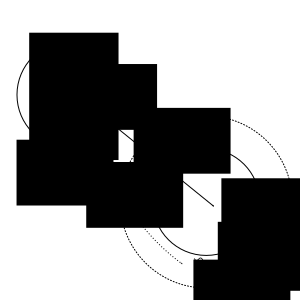
\includegraphics{img/error_map.pdf}
    \caption{Map of the error with $\tilde f$ instead of $f$}
    \label{img:error-map}
  \end{center}
\end{figure}

\paragraph{Stability of the componentwise forward analysis}

\index{Stability indicator}
\begin{definition}[Forward stability]
  Let $\tilde f$ be the floating point implementation of an algorithm to solve problem $(f, x)$ of relative normwise condition $\kappa_{\operatorname{rel}}$.
  The \emph{stability indicator} of a normwise forward analysis is the smallest number $\sigma \geq 0$, such that for all $\tilde x \in E$ it holds that
  \[ \frac{\Norm{\tilde f(\tilde x) - f(\tilde x)}}{\Norm{f(\tilde x)}} \leq \sigma \kappa_{\operatorname{rel}} \varepsilon \qquad \text{ for } \varepsilon \to 0 \]
\end{definition}

$\overline{\kappa}_{\operatorname{rel}}$ is the smallest number $\sigma \geq 0$ such that
\[ \max_i \frac{\Abs{\tilde f_i(\tilde x) - f_i(\tilde x)}}{\Abs{f_i(\tilde x)}} \dotted{\leq} \sigma \cdot \overline{\kappa}_{\operatorname{rel}} \varepsilon \qquad \text{ for } \varepsilon \to 0 \]
where $\overline{\kappa}_{\operatorname{rel}}$ is the componentwise relative conditioning of $(f, x)$.
\index{Stable algorithm}
We call algorithm $\tilde f$ \emph{stable} in regards of forward analysis if $\sigma$ is smaller than the number of consecutively executed elementary operations.

\begin{lemma}
  For the elementary operations $\Set{+, -, \cdot, /}$ and the floating point implementations $\Set{\hat{+}, \hat{-}, \hat{\cdot}, \hat{/}}$ it holds that $\sigma \kappa_{\operatorname{rel}} \leq 1$.
\end{lemma}
\begin{proof}
  For every floating point implementation it holds that
  \[ x \hat{*} y = (x * y)(1 + \delta) \qquad * \in \Set{+, -, \cdot, /} \]
  by Lemma~\ref{lemma:2-4} for some $\delta$ with $\Abs{\delta} \leq \varepsilon$.
  Thus,
  \[ \frac{\Abs{x \hat{*} y - x * y}}{x * y} = \frac{\Abs{(x * y)(1 + \delta) - x * y}}{\Abs{x * y}} = \Abs{\delta} \leq 1 \cdot \varepsilon \]
\end{proof}

This approach is rather impractical (determination of the conditioning number of the problem is difficult).

\paragraph{Stability of the componentwise backwards analysis}

\begin{figure}[!ht]
  \begin{center}
    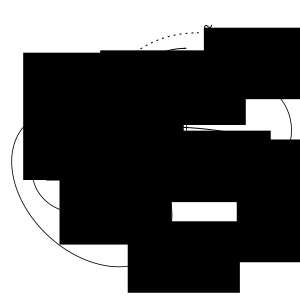
\includegraphics{img/backwards-analysis.pdf}
    \caption{Backwards analysis}
    \label{img:backwards-analysis}
  \end{center}
\end{figure}

\index{Unstable algorithm}
\textbf{Idea:} interpret the error in the algorithm like an input error.
The result $\tilde y = \tilde f(\tilde x)$ is considered as the exact result $\tilde y = f(\hat{x})$ for distorted data $\hat{x}$.
$E = \SetDef{\tilde x}{\Norm{\tilde x - x} \leq \varepsilon \Norm{x}}$.
This is only possible if $\tilde y$ is a admissible solution of $f$ at all.
In the other case, we call the algorithm \emph{unstable}.

\index{Normwise backwards error}
\index{Stability indicator}
\begin{definition}
  The \emph{normwise backwards error} of the algorithm $\tilde f$ to solve the problem $(f, x)$ is the smallest number $\eta \geq 0$,
  for which $\forall \tilde x \in E_\varepsilon$ some $\hat{x}$ exists such that
  \[ \frac{\Norm{\hat{x} - \tilde x}}{\Norm{\tilde x}} \dotted{\leq} \eta \qquad \text{ for } \varepsilon \to 0 \]
  The \emph{componentwise backwards error} is defined as
  \[ \max_i \frac{\Abs{\hat{x}_i - \tilde{x}_i}}{\Abs{\tilde x_i}} \dotted{\leq} \eta \qquad \text{ for } \varepsilon \to 0 \]
  The algorithm is called \emph{stable} (in regards of backwards analysis) with respect to the relative input error $\varepsilon$ if $\eta < \varepsilon \cdot \text{ number of elementary operations}$.
  For given $\varepsilon$ we define a \emph{stability indicator} of the backwards analysis as quotient
  \[ \sigma_R \coloneqq \frac{\eta}{\varepsilon} \]
\end{definition}

\begin{lemma}
  \label{lemma:2-15}
  For stability indicators $\sigma$ and $\sigma_R$, of the forward/backward analysis respectively, it holds that $\sigma \leq \sigma_R$.
  Especially by backwards stability, forwards stability follows.
\end{lemma}
\begin{proof}
  By definition of the backwards error, for every $\tilde x \in E$ there exists some $\hat{x}$ such that $f(\hat{x}) = \tilde f(\tilde x)$ and
  \[ \frac{\Norm{\hat{x} - \tilde x}}{\Norm{\tilde x}} \dotted{\leq} \eta = \sigma_R \cdot \varepsilon \qquad \text{ for } \varepsilon \to 0 \]
  For the relative error in the result, we have
  \[ \frac{\Norm{\tilde f(\tilde x) - f(\tilde x)}}{\Norm{f(\tilde x)}} = \frac{\Norm{f(\hat{x}) - f(\tilde x)}}{\Norm{f(\tilde x)}} \dotted{\leq} \kappa_{\operatorname{rel}} \frac{\Norm{\hat{x} - \tilde{x}}}{\Norm{\tilde{x}}} \dotted{\leq} \kappa_{\operatorname{rel}} \cdot \sigma_R \cdot \varepsilon \qquad \text{ (for $\varepsilon \to 0$)} \]
\end{proof}
\begin{Remark}
  $Ax = b$ with solution $\tilde x$, approximation $\hat{x}$.
  Error $\Norm{\hat{x} - \tilde x}$ is not computable, because $\tilde x$ is unknown.
  Residue $\Norm{b - A\hat{x}}$.
\end{Remark}

\subsection{Backwards analysis for linear equation systems}
\label{sec:2-4}

\textbf{Question:} Is the LU decomposition a backwardsstable algorithm?

In the following, we will use the following notation for vectors and matrices:
\[ \Abs{A} \leq \Abs{B} \iff \Abs{a_{ij}} \leq \Abs{b_{ij}} \forall i,j \]

\begin{lemma}
  \label{lemma:2-16}
  The floating point implementation of the scalar product
  \[ \IP{x}{y} \coloneqq x_n y_n + \IP{x^{n-1}}{y^{n-1}} \]
  with $x^{n-1} \coloneqq (x_1, \dots, x_{n-1})^T$ and $y^{n-1} \coloneqq (y_1, \dots, y_{n-1})^T$
  denotes some solution $\IP{x}{y}_{\text{rd}} \coloneqq \operatorname{rd}(\IP{x}{y})$ for some $x, y \in \mathbb R^n$
  such that $\IP{x}{y}_{\operatorname{rd}} = \IP{\hat{x}}{y}$ for some $\hat{x} \in \mathbb R^n$ with $\Abs{x - \hat{x}} \dotted{\leq} n \varepsilon \Abs{x}$,
  hence the relative componentwise backwards error is $\eta \leq n \cdot \varepsilon$
  and the scalar product is stable in regards of backwards analysis (with $2n-1$ elementary operations by the scalar product). % TODO too long sentence
\end{lemma}
\begin{proof}
  We need to prove:
  \[ \forall i: \Abs{x_i - \hat{x}_i} \leq \underbrace{n \varepsilon \Abs{x_i}}_{h(\varepsilon)} + \overbrace{\sigma(\Norm{h(\varepsilon)})}^{\sigma} \qquad \text{ for $\varepsilon \to 0$ with } \lim_{\varepsilon \to 0} \frac{\Norm{\varphi(\varepsilon)}}{\Norm{h(\varepsilon)}} = 0 \]
  Thus, we look for a function that converges superlinear towards $0$ for $\varepsilon \to 0$ ($\mathcal O(\varepsilon)$).

  We use induction over $n$ to prove this.
  For $n=1$, the statement is true by Lemma~\ref{lemma:2-4}.
  Now let $n > 1$ and let the statement be true for $n - 1$. For floating point implementation of recursion it is true that
  \[ {\IP xy}_{\operatorname{rd}} = (x_n y_n (1 + \delta) + \IP{x^{n-1}}{y^{n-1}}_{\operatorname{rd}}) (1 + \tilde{\delta}) \]
  where $\Abs{\delta} \leq \varepsilon$ and $\Abs{\tilde \delta} \leq \varepsilon$ characterize the relative error of multiplication and addition respectively.

  By the induction hypothesis, it holds that $\IP{x^{n-1}}{y^{n-1}}_{\operatorname{rd}} = \IP{z}{y^{n-1}}$ for some $z \in \mathbb R^{n - 1}$ with
  \[ \Abs{x^{n-1} - z} \leq (n - 1) \varepsilon \Abs{x^{n-1}} + \mathcal O(\varepsilon) \]
  By $\hat{x}_n = x_n (1 + \delta)(1 + \tilde\delta)$ and $\hat{x}_k = z_k (1 + \tilde\delta)$ by $k = 1, \dots, n-1$ it follows that
  %\[ \Norm{x^{n-1} - z} \leq (n - 1) \varepsilon \Abs{x^{n-1}} \]
  %With $\hat{x_n} = x_n(1 + \delta)(1 + \tilde \delta)$ and $\hat{x}_{\kappa} = z_k(1 + \tilde \delta)$ for $k = 1, \dots, n-1$ it follows that
  \begin{align*}
    {\IP xy}_{\operatorname{rd}} &= x_n y_n(1 + \delta)(1 + \tilde \delta) + \IP{z(1 + \varepsilon)}{y^{n-1}} \\
      &= \hat{x}_n y_n + \IP{\hat{x}^{n-1}}{y^{n-1}} = \IP{\hat{x}}{y} \\
      &\text{ with } \Abs{x_n - \hat{x}_n} \leq 2 \varepsilon \Abs{x_n} + \Abs{x_n} \Abs{y_n} \delta \tilde \delta \\
      &\leq n \varepsilon \Abs{x_n} + \mathcal O(\varepsilon) \\
    \text{ and } \Abs{x_k - \hat x_k} &\leq \Abs{x_k - z_k} + \Abs{x_k - \hat{x}_k} \\
      &\leq (n - 1) \varepsilon \Abs{x_k} + \mathcal O(\varepsilon) + \varepsilon \Abs{z_k} \\
      &\leq n \varepsilon \Abs{x_k} + \mathcal O(\varepsilon) \text{ for } k = 1, \dots, n-1
  \end{align*}
  The last estimate can be made using
  \[ \Abs{z_k} - \Abs{x_k} \leq \Abs{x_k - z_k} \leq (n - 1) \varepsilon \Abs{x_k} + \mathcal O(\varepsilon) \]
  \[ \implies \varepsilon \Abs{z_k} \leq \varepsilon \Abs{x_k} + \mathcal O(\varepsilon) \]
\end{proof}

\begin{thm}
  \label{theorem:2-17}
  The floating point implementation of forward substitution to solve a linear equation system $Lx = b$ with some lower triangular matrix $L$ computes the solution $\hat{x}$ such that there exists some lower triangular matrix $\hat L$ with $\hat L \hat x = b$ and $\Abs{L - \hat L} \dotted{\leq} n \varepsilon \Abs{L}$.
  Hence for componentwise relative backwards errors, we have $\eta \leq n \cdot \varepsilon$ and the forward substitution is stable in regards of backwards analysis.
\end{thm}
\begin{proof}
  Again, we will use a recursive approach.
  \[ l_{kk} x_k = b_k - \IP{l^{k-1}}{x^{k-1}} \]
  For $k = 1, \dots, n$, we have
  \begin{align*}
    x^{k-1} &\coloneqq (x_1, \dots, x_{k-1})^T \text{ and } \\
    l^{k-1} &\coloneqq (l_{k,1}, \dots, l_{k,k-1})^T
  \end{align*}
  In floating point arithmetics, the following recursion is yielded,
  \[ l_{kk}(1 + \delta_k)(1 + \tilde \delta_k) \hat{x}_k = b_k - \IP{l^{k-1}}{x^{k-1}}_{\operatorname{rd}} (1 + \tilde \delta_k) \]
  where $\delta_k, \tilde \delta_k$ with $\Abs{\delta_k} \leq \varepsilon$ and $\Abs{\tilde\delta_k} \leq \varepsilon$ are the relative errors of multiplication/addition.
  By Lemma~\ref{lemma:2-16}, it follows that
  \[ \IP{l^{k-1}}{\hat{x}^{k-1}}_{\operatorname{rd}} = \IP{\tilde l^{k-1}}{\hat{x}^{k-1}} \]
  for some vector $\tilde l^{\tilde k - 1} = (\tilde l_{k,1}, \dots, \tilde l_{k,k-1})^T$
  with $\Abs{l^{k-1} - \tilde l^{k-1}} \dotted{\leq} (k - 1) \varepsilon \Abs{l^{k-1}}$.
  Now let $\hat{l}_{kk} \coloneqq l_{kk} (1 + \delta_k)(1 + \tilde \delta_k)$ and $\hat{l}^{k-1} \coloneqq (1 + \tilde \delta_k) \tilde l^{k-1}$ then
  \begin{align*}
    \Abs{\hat{l}^{k-1} - l^{k-1}} &\dotted{\leq} (k-1) \varepsilon \Abs{l^{k-1}} + \Abs{\tilde \delta_k} \Abs{\tilde l^{k-1}} \\
      &\dotted{\leq} k \varepsilon \Abs{l^{k-1}} \\
    \Abs{\hat{l}_{kh} - l_{kj}} &\dotted{\leq} 2 \varepsilon
  \end{align*}
  \[ \implies \hat{L} \hat{x} = b \land \Abs{L - \hat{L}} \dotted{\leq} n \varepsilon \Abs{L} \]
\end{proof}

\dateref{2018/10/18}

\begin{lemma}
  \label{lemma:2-18}
  Let $A$ have a LU decomposition. Then Gaussian elimination determines $\hat L$ and $\hat U$ such that $\hat L \hat U = \hat A$ for some matrix $\hat A$ with
  \[ \Abs{A - \hat A} \dotted{\leq} n \Abs{\hat L} \Abs{\hat U} \varepsilon \]
\end{lemma}

\begin{thm}
  \label{theorem:2-19}
  $A$ has some LU-decomposition. 
  Then Gaussian elimination for linear equation system $Ax = b$ gives a solution $\hat x$ with $\hat A \hat x = b$ for some matrix $\hat A$ with
  \[ \Abs{A - \hat A} \dotted{\leq} 2n \Abs{\hat L} \Abs{\hat U} \varepsilon \]
\end{thm}

\begin{thm}
  \label{theorem:2-20}
  The Gaussian elimination with column pivot strategy for the linear equation system $Ax = b$ determines some $\hat x$ such that $\hat A \hat x = b$ for some matrix $\hat A$ with
  \[ \frac{\Norm{A - \hat A}_{\infty}}{\Norm{A}_\infty} \dotted{\leq} 2n^3 \rho_n(A) \varepsilon \qquad \text{ where } \rho_n(A) \coloneqq \frac{\alpha_{\operatorname{max}}}{\max_{i,j} \Abs{a_{ij}}} \]
  and where $\alpha_{\operatorname{max}}$ is the largest absolute value of an element that occurs during elimination in the remainder matrices $A^{(1)} = A$ to $A^{(n)} = U$.
\end{thm}

\[ A = \begin{bmatrix} 1 & 0 & \dots & 0 & 1 \\ -1 & \vdots & \ddots & \vdots & \vdots \\ \vdots & \ddots & \ddots & & \\ -1 & \dots & \dots & -1 & 1 \end{bmatrix} \]
For matrix $A$ it holds that $\rho_n(A) = 2^{n-1}$.

Consider that the previous result also provides \emph{no} positive statement about the backwards stability of the LU decomposition.

\section{Linear least squares}

\textbf{Goal:} Solution of overdetermined linear equation systems
\[ Ax = b \qquad A \in \mathbb R^{m \times n} \qquad m > n \qquad b \in \mathbb R^m \]
by the method of linear least squares.

For this, we are going to use (numerically stable) orthogonal transformations.

\subsection{Gaussian process of least squares}

\textbf{Problem:} Given $m$ input data points ($t_i, b_i$) and $t_i, b_i \in \mathbb R$ for $i = 1, \dots, m$.
They describe the values $b_i$ of an object at timestamp $t_i$.

\index{Modelling function}
We assume that there exists an underlying law such that the dependency of $b$ and $t$ can be represented by some \emph{modelling function} $\varphi$ with $b(t) = \varphi(t_i; x_1, \dots, x_n)$. The modelling function therefore takes $n$ unknowns $p_i$.

\begin{example}[Ohm's law]
  Consider Ohm's law $b = xt = \varphi(t_i x)$ where $t$ denotes the current, $b$ the voltage and $x$ resistance.
\end{example}

So want to approximate data points in the $\mathbb R^2$ plane linearly.

If the model would be \emph{exact} and if you have no errors in measurement, then we are supposed to evaluate parameters $x_1, \dots, x_n$ such that $b_i = b(t_i) = \varphi(t_i; x_1, \dots, x_n)$ for $i = 1, \dots, m$.

In reality, measurements are subject to errors and modelling functions are also just approximations of reality.
We therefore require that $b_i \approx \varphi(t_i; x_1, \dots, x_n)$ for $i = 1, \dots, m$.
We weight the individual deviations
\[ \Delta i \coloneqq b_i - \varphi(t_i; x_1, \dots, x_n) \qquad i = 1, \dots, m \]
By Gauss, determine $x_i$ such that $\sum_{i=1}^m \Delta i^2$ becomes minimal.
We use the short notation $\Delta^2 \coloneqq \sum_{i=1}^m \delta_i^2 \implies \operatorname{min}$.
Often it is more useful to weight the individual deviations differently.
For some measurement precision $\delta b$, introduce weights
\[ \sum_{i=1}^m \left(\frac{\Delta i}{\delta b_i}\right) \to \text{ min} \]
We consider the special case of linear (with respect to $x$) modelling functions $\varphi$, hence $\varphi(t_i; x_1, \dots, x_n) = a_1(t) x_1 + \dots + a_n(t) x_n$ where $a_1, \dots, a_n: \mathbb R \to \mathbb R$ are arbitrary functions.
Furthermore we choose $\Norm{} = \Norm{}_2$.
We can denote the least square problem as
\[ \Norm{b - Ax} \to \operatorname{min} \qquad \text{ where } b = \begin{pmatrix} b_1 \\ \vdots \\ b_m \end{pmatrix}, x = \begin{pmatrix} x_1 \\ \vdots \\ x_n \end{pmatrix} \]
\[ \text{and } A = (a_{ij}) \in \mathbb R^{m \times n} \text{ with } a_{ij} \coloneqq a_j(t_i) \]

% TODO why are the following enumerations made with 3 indices?
\subsection*{Orthogonal equations}

We look for some point $z = Ax$ of the image space $U(A)$ of $A$, that has the smallest distance to some given $b$.
$Ax$ is the orthogonal projection of $b$ to the subspace $U(A) = \operatorname{image}(A)$.

\begin{thm}
  \label{theorem:3-2}
  Let $V$ be a vector space of $\dim{V} < \infty$ with scalar product $\IP{}{}$.
  Let $U \subset V$ be a subspace. Let
  \[ U^\bot = \SetDef{v \in V}{\IP{v}{u} = 0 \forall u \in U} \]
  be the orthogonal complement in $V$. Then for all $v \in V$ with respect to the norm induced by $\Norm{v} = \sqrt{\IP vv}$ such that
  \[ \Norm{v - u} = \min_{\tilde u \in U} \Norm{v - \tilde u} \iff v - u \in U^\bot \]
\end{thm}

Proof sketch:
\begin{itemize}
  \item $V = U \oplus U^\bot$
  \item $v = u + w, u \in U, w \in U^\bot$ unique
  \item $\tilde u \in U$ arbitrary:
    \[ \Norm{v - \tilde u}^2 = \Norm{(v - u) + (u - \tilde u)}^2 = \Norm{v - u}^2 + \Norm{u - \tilde u}^2 \geq \Norm{v - u}^2 \]
    with $v - u = w$ and $(u - \tilde u) \in U$.
\end{itemize}

\dateref{2018/10/23}

\index{Orthogonal projection}
The unique solution $u \in U$ of $\min{\Norm{v - u}}$ is called \emph{orthogonal projection} of $V$ to $U$.
The map $P: V \to U$ with $v \mapsto Pv$ with $Pv = u$ is linear and is called \emph{orthogonal projection} of $V$ to $U$.

\begin{remark}
  \label{rem-3-3}
  We get an analogous statement if we replace $U$ by an affine subspace $W = w_0 + U \subseteq V$ where $w_0 \in V$.
  $U$ is the parallel, to $W$, linear subspace of $V$.

  For all $v \in V$, $w \in W$: $\Norm{v - w} = \min_{\tilde w \in w} \Norm{v - \tilde w} \iff v-w \in U^\bot$.
\end{remark}

\index{Orthogonal equations}
\begin{thm}
  \label{theorem:3-4}
  The vector $x \in \mathbb R^n$ is a solution of the linear least squares problems $\min{\Norm{b - Ax}} \iff x$ satisfies the so-called orthogonal equations $A^T Ax = A^T b$~\dt{Normalengleichungen}.

  Especially, the linear least squares problem is uniquely solvable iff $A$ has full column rank.
\end{thm}

\begin{proof}
  By Theorem~\ref{theorem:3-2}, $V \coloneqq \mathbb R^n$, $U \coloneqq \operatorname{image}(A) = \operatorname{rank}(A)$.
  \begin{align*}
    \implies \max{\Norm{b - Ax}} &\iff \IP{b - Ax}{A \tilde x} = 0 \forall \tilde x \in \mathbb R^n \\
      &\iff 0 = \IP{A^t (b - Ax)}{\tilde x} \forall \tilde x \in \mathbb R^n \\
      &\iff A^t (b - Ax) = 0 \\
      &\iff A^t b = A^t Ax
  \end{align*}
  Thus the first statement is proven. How about the second statement?
  \begin{align*}
    A^t A \text{ regular } &\iff \operatorname{rank}(A) = n
  \end{align*}
\end{proof}

\begin{Remark}[Geometric interpretation]
  $b - Ax$ is orthogonal to $\operatorname{range}(A)$ with $A \subseteq \mathbb R^n$.
\end{Remark}

\textbf{Solution of the orthogonal equation system:}
Theoretically, we can create $A^T A$ and retrieve a symmetric positive definite matrix ($\implies$ decomposition with Cholesky process).

\begin{Remark}[Computing time]
  \begin{enumerate}
    \item Determination of $A^t A$ (only one half, because of symmetry)
      \[ (A^t A)_{ij} = (\IP{a_j}{a_j})_{i,j} \qquad a_j = j\text{-th column of } A \to \frac12 n^2 n \]
    \item Cholesky decomposition $\sim \frac16 n^3$
  \end{enumerate}
  In case of $m \gg n$, the first approach will take over $\implies \sim \frac12 n^2 n$. $\frac23 m^3$ for $n \approx m$.
\end{Remark}

\begin{lemma}
  \label{lemma:3-5}
  For some matrix $A \in \mathbb R^{m \times n}$ with $m \geq n$ and full column rank ($\operatorname{rank}(A) = n$),
  $\kappa_2(A^t A) = (\kappa_2(A))^2$.
\end{lemma}

\begin{proof}
  By definition of condition numbers:
  \begin{align*}
    (\kappa_2(A))^2 &= \frac{\max_{\Norm{x}=1} \Norm{Ax}_2^2}{\min_{\Norm{x} = 1} \Norm{Ax}_2^2} \\
      &= \frac{\max_{\Norm{x}=1} \IP{Ax}{Ax}}{\min_{\Norm{x} = 1} \IP{Ax}{Ax}} \\
      &= \frac{\max \IP{A^t Ax}{x}}{\min \IP{A^t Ax}{x}} & \text{\enquote{Rayleigh eigenvalue}} \\
      &\overset{A^tA \text{sym.}}{=} \frac{\lambda_{\operatorname{max}} (A^t A)}{\lambda_{\operatorname{min}} (A^t A)} \\
      &\overset{A^tA \text{sym.}}{=} \kappa_2(A^t A)
  \end{align*}
\end{proof}

Recognize that the amplification of the error for the orthogonal equation is larger.
Therefore it makes sense to avoid computing $A^T A$ and use the original matrices $A$ and $A^T$ instead, e.g.
\[ \begin{pmatrix} I & A \\ A^T & 0 \end{pmatrix} \begin{pmatrix} r \\ 0 \end{pmatrix} = \begin{pmatrix} b \\ 0 \end{pmatrix} \]
\[ \implies A^T r = 0 \land r \neq Ax = b \]
\[ \implies r = b - Ax \qquad \implies 0 = A^T r = A^T (b - Ax) \]

\[ \Norm{A_3}_2^2 = \max_{\Norm{x}_2 = 1} \Norm{Q_j x}_2^2 = \max_{\Norm{x}_2 = 1} \IP{x}{Q^TQx} = 1 \]
Recognize that $Q^TQ = I$.

\subsection{Orthogonalization process}

We can represent the eliminination process for linear equation systems  (e.g. Gaussian elimination) formally as
\[ A \xrightarrow{f_1} B_1 A \xrightarrow{f_2} B_2 B_1 A \xrightarrow{f_3} \dots \xrightarrow{f_k} B_k \dots B_1 A \dots \rightarrow U \]
where
\[ U = \begin{pmatrix} 1 & * \\ 0 & \varepsilon \end{pmatrix} \]
and where matrices $B_j$ describe the operations applied to matrix $A$.
Through this process, the condition numbers of the individual matrices can be amplified, such that instabilities can occur.
If we instead use orthogonal transformations $Q_j$ for elimination, we have
\[ \kappa_2(Q_j) = \Norm{Q_j}_2 \cdot \Norm{Q_j}^{-1}_2 = \Norm{Q_j}_2 \Norm{Q_j}_2 = 1 \]

Orthogonalization process are necessarily stable, but have higher computing times compared to Gaussian elimination.
If we assume we transformed a given matrix $A \in \mathbb R^{m \times n}$ with $m \geq n$ with some orthogonal matrix $Q \in \mathbb R^{m \times m}$ into upper triangular matrix, then
\[
  Q^T A = \begin{bmatrix}
    *      & \dots   & x \\
           & \ddots  & \vdots \\
           &         & x \\
    0      &         & * \\
    \vdots &         & \vdots \\
    0      &         & 0
  \end{bmatrix} = \begin{bmatrix} U \\ 0 \end{bmatrix}
\]

\begin{thm}
  \label{theorem:3-6}
  Let $A \in \mathbb R^{m \times n}$, $m \geq n$, of maximum rank $n, b \in \mathbb R^m$ and $Q \in \mathbb R^{m \times m}$ be an orthogonal matrix with
  \[ Q^T A = \begin{bmatrix} U \\ 0 \end{bmatrix} \text{ and } Q^T b = \begin{bmatrix} b_1 \\ b_2 \end{bmatrix} \]
  where $b_1 \in \mathbb R^n$, $b_2 \in \mathbb R^{m - n}$ and $U \in \mathbb R^{n \times n}$ is an (invertible) upper triangular matrix.
  Then $x = U^{-1} b_1$ is the solution of the linear least squares problems $\min\Norm{b - Ax}_2$.
\end{thm}

\begin{proof}
  Because $Q$ is orthogonal, $\forall x \in \mathbb R^n$ it follows that
  \[ \Norm{b - Ax}_2^2 = \Norm{Q^T (b - Ax)}_2^2 = \Norm{\begin{pmatrix} b_1 - Ux \\ b_2 \end{pmatrix}}_2^2 = \Norm{b_1 - Ux}_2^2 + \Norm{b_2}_2^2 \geq \Norm{b_2}_2^2 \]
  Because $\rank(A) = \rank(U) = n$, $U$ is invertible. The term $\Norm{b_1 - Ux}_2^2$ disappear for $x = U^{-1} b_1$
\end{proof}

\begin{Remark}
  $A$: $0 \neq \Norm{r} = \Norm{b - Ax} = \Norm{b_2}$.
\end{Remark}

What do orthogonal transformations look like?
In general, these transformations are rotations and reflections.

e.g. $x \mapsto \alpha e_1 = Qx$ with $Q = \begin{bmatrix} \cos(\theta) & \sin(\theta) \\ -\sin(\theta) & \cos(\theta) \end{bmatrix}$.

Alternatively, $x \mapsto \alpha e_1 = x = 2\frac{\IP vx}{\IP vv} v$ where $v$ is collinear to the difference $x = \alpha e_1$.

\subsection*{Givens rotations}

\index{Givens rotations}
Givens rotations are described by matrices of form
\[
  Q_{k,l} \coloneqq \begin{bmatrix}
    I &    &   &   & \\
      & c  &   & s & \\
      &    & I &   & \\
      & -s &   & c & \\
      &    &   &   & I
  \end{bmatrix}
  \in \mathbb R^{m \times m}
\]
with proper dimension of the unit matrix and $c^2 + s^2 = 1$. For $x \in \mathbb R^m$ it holds that
\[
  x \mapsto y = Q_{k,l} x \text{ with } y_i = (Q_{k,l} x)_i =
  \begin{cases}
    c x_k + sx_l & i = k \\
    -s x_k + cx_l & i = l \\
    x_i & \text{else}
  \end{cases}
\]
Thus for $A = [a_1, \dots, a_n] \in \mathbb R^{m \times n}$, we get
\[ Q_{k,l} A = [Q_{k,l} a_1, \dots, Q_{k,l} a_n] \]
Hence, only rows $k$ and $l$ of matrix $A$ will be modified.

\textbf{Question:} How to choose $c$ and $s$ to eliminate a component $x_l$ of $x$?
Because $Q_{k,l}$ operates on the $(k,l)$-layer, we consider without loss of generality $m=2$.
By $x_k^2 + x_l^2 \neq 0$ and $s^2 + c^2 = 1$ it follows that
\[ \begin{bmatrix} c & s \\ -s & c \end{bmatrix} \begin{bmatrix} x_k \\ x_l \end{bmatrix} = \begin{bmatrix} r \\ 0 \end{bmatrix} \]
\[ \iff r = \pm \sqrt{x_k^2 + x_l^2}, c = \frac{x_k}{r}, s = \frac{x_l}{r} \]
Computing $x_k^2$ might gives us an exponent overflow.
\[ \tau \coloneqq \frac{x_k}{x_l}, s \coloneqq \frac{1}{\sqrt{1 + \tau^2}}, c \coloneqq s\tau \text{ if } \Abs{x_l} > \Abs{x_k} \]
and accordingly,
\[ \tau \coloneqq \frac{x_l}{x_k}, c = \frac{1}{\sqrt{1 + \tau^2}}, s \coloneqq c\tau \text{ if } \Abs{x_k} \geq \Abs{x_l} \]
Now transform $A$ iteratively into triangular form.

For example, consider
\[ A = \begin{bmatrix} A & * & * & * \\ * & * & * & * \\ * & * & * & * \\ * & * & * & * \\ * & * & * & * \end{bmatrix} \xrightarrow{(5,4)} \begin{bmatrix} * & * & * & * \\ * & * & * & * \\ * & * & * & * \\ * & * & * & * \\ 0 & * & * & * \end{bmatrix} \xrightarrow{(4,3)} \dots \]
\[ \xrightarrow{(2,1)} \begin{bmatrix} * & * & * & * \\ 0 & * & * & * \\ 0 & * & * & * \\ 0 & * & * & * \\ 0 & * & * & * \end{bmatrix} \xrightarrow{(5,4)} \dots \xrightarrow{(4,3)} \dots \xrightarrow{(5,4)} \begin{bmatrix}  * & * & * & * \\ 0 & * & * & * \\ 0 & 0 & * & * \\ 0 & 0 & 0 & * \\ 0 & 0 & 0 & 0 \end{bmatrix} \]
\begin{Remark}[Computing time]
  Computing time for a dense matrix $A \in \mathbb R^{m \times n}$:
  \begin{enumerate}
    \item $\sim \frac{n^2}{2}$ square roots and $\frac43 n^3$ multiplications, if $m \approx n$.
    \item $m \cdot n$ are square root and $2mn^2$ multiplications if $m \ggg n$.
  \end{enumerate}
\end{Remark}
This is an alternative for Gaussian elimination. The algorithm is \emph{more stable}, but \emph{more expensive}.

But it can be advantageous for special matrix, e.g. Hessenberg matrices, which are \enquote{almost triangular} (so the first subdiagonal also contains non-zero entries).
Here, we need $n-1$ Givens rotations if we want to achieve upper triangular form.

\subsection*{Householder reflections}
\dateref{2018/10/25}

\index{Householder reflections}
For given $0 \neq v \in \mathbb R^m$, we define the matrix $Q \in \mathbb R^{m \times m}$.
\[ Q = I - 2 \frac{vv^T}{v^Tv} \]

They describe reflections on the mirror plane, which are vertical to $v$.
The following properties hold:
\begin{enumerate}
  \item symmetry: $Q = Q^T$
  \item orthogonality: $QQ^T = I$
  \item $Q^2 = \operatorname{id}$, thus $Q$ is \emph{involutional}
  \item $\operatorname{spec}(Q) = \Set{\pm 1}, -1$ simple, $1$ $(n-1)$-times.
\end{enumerate}

For $y \in \mathbb R^n$,
\[ y \mapsto Qy = \left(I - 2 \frac{vv^T}{v^T v}\right) y = y - 2 \cdot \frac{\IP vy}{\IP vv} \]

\textbf{Question}: How can we achieve that $Q$ maps vector $y$ to $\alpha \cdot e_1$? Hence,
\[ \alpha \cdot e_1 = y - 2 \frac{\IP vy}{\IP vv} \cdot v \in \operatorname{span}(e_1) = \alpha(\Set{e_1}) \]

Consider that
\[ \Abs{\alpha} = \Norm{\alpha e_1} = \Norm{y - 2 \frac{\IP vy}{\IP vv} v}_2 = \Norm{Qy}_2 = \Norm{y}_2 \]
and $y \in \operatorname{span}(y - \alpha \cdot e_1)$.
This way we can retrieve $Q$ by,
\[ v \coloneqq y - \alpha e_1 \qquad \alpha = I \Norm{y}_2 \]
To avoid elimination (or subtraction) in $v = (y_1 - \alpha, y_2, \dots, y_n)^T$, choose $\alpha \coloneqq -\operatorname{sign}(y_1) \cdot \Norm{y}_2$. Now,
\[ \IP vv = \IP{y - \alpha e_1}{y - \alpha e_1} = \Norm{y}^2 - 2\alpha \IP{e_1}{y} + \alpha^2 = 2\alpha^2 - 2\alpha \IP{e_1}{y} = -2\alpha (y_1 - \alpha) \]
$Qy$ for $y \in \mathbb R^m$ can be determined by
\[ Qy = y - 2 \frac{\IP vy}{2(y_1 - \alpha)} \cdot v \]
In a first step choose $Q_1$ (where $A \in \mathbb R^{m \times n}$):
\[ [a_1 \dots a_n] = A \to A' = Q_1 \cdot A = \begin{bmatrix} \alpha_1 & \\ 0 & \\ \vdots & a_2' \dots a_n' \\ 0 & \end{bmatrix} \]
where $Q_1 = I - 2 \frac{v_1 v_1^T}{v_1^T v_1}$ with $v_1 \coloneqq a_1 - \alpha_1 e_1$ and $\alpha_1 \coloneqq -\operatorname{sign}(a_{11}) \cdot \Norm{a_1}$.

After the $k$-th step, we get
\[ A^{(k)} = \begin{bmatrix} * & & & * \\ & \ddots & & \\ & & * & \\ 0 & & & T^{(k+1)} \end{bmatrix} \]
with $T^{(k+1)} \in \mathbb R^{m-k \times n-k}$. Now we create orthogonal matrix
\[ Q_{k+1} \coloneqq \begin{bmatrix} I & 0 \\ 0 & \tilde Q_{k+1} \end{bmatrix} \]
where $\tilde Q_{k+1}$ modifies matrix $T^{(k+1)}$. The next subcolumn will be eliminated.

After $p = \min(m,n)$ steps, we retrieve an upper triangular matrix
\[ R = Q_p \dots Q_1 \cdot A \]
\[ \iff A = QR \text{ where } Q = Q_1 \cdot \dots \cdot Q_p \]

% TODO static reference
Based on Theorem~2.6, we retrieve the following process:
\begin{enumerate}
  \item $A = QR$ ($QR$ decomposition using Householder or Givens)
  \item $\begin{pmatrix} b_1 \\ b_2 \end{pmatrix} = Q^t b$ with $b_1 \in \mathbb R^n$ and $b_2 \in \mathbb R^{m-n}$ (transformation of $b$)
  \item $Rx = b_1$ (solving by backwards substitution)
\end{enumerate}

\begin{Remark}[Implementation]
  Usually, we store the Householder vectors $v_1, \dots, v_p$ in the lower half of $A$ and the diagonal elements $v_{1i} = \alpha_i$ with $i = 1,\dots,p$ in a separate vector.
\end{Remark}

\begin{Remark}[Computing time]\hfill{}
  \begin{itemize}
    \item $\sim 2n^2m$ multiplications if $m \gg n$
    \item $\frac23 n^3$ if $m \approx n$
  \end{itemize}
\end{Remark}

It is important to recognize that this process is numerically stable!

\subsection{Singular value decomposition} % TODO chapter 3.3

Literature:
\begin{itemize}
  \item Gene H. Golub and Charles F. Van Loan: \enquote{Matrix computations}
\end{itemize}

If $A \in \mathbb R^{m \times n}$ has non-full rank $n$,
then the linear equation system of $\min \Norm{b - Ax}$ is not unique,
because $\forall \tilde x: \Norm{b - A\tilde x} = \Norm{b - A(\tilde x + v)} \forall v \in \ker(A)$.

Are there more decompositions of the matrix?

Recognize that the QR decomposition always exists anyways.

\begin{thm}
  \label{theorem:3-7}
  Let $A \in \mathbb R^{m \times n}$.
  There $\exists U \in \mathbb R^{m \times m}, V \in \mathbb R^{n \times n}:
  U^T U = I, V^T V = I$ and $A = U \Sigma V^T$ with $\Sigma \in \mathbb R^{n \times n}$
  where $\Sigma = \operatorname{diag}(\sigma_1, \dots, \sigma_p), p = \min(m, n), V = [v_1, \dots, v_n]$
  and $\sigma_1 \geq \sigma_2 \geq \dots \geq \sigma_p \geq 0$.
\end{thm}

\index{Singular values of a matrix}
\index{Singular vectors of a matrix}
\begin{remark}
  $\sigma_i$ are called \enquote{singular values} of $A$.
  $u_i$ and $v_i$ are called left- and right-singular vectors of $A$.
\end{remark}

\dateref{2018/10/30}

\begin{proof}
  Let $x \in \mathbb R^n$ and $y \in \mathbb R^m$ such that $\Norm{x}_2 = 1 = \Norm{y}_2$ and $Ax = \sigma y$ where $\sigma = \Norm{A}_2$.
  Recognize that $x,y$ exist because $\Norm{A}_2 = \sup_{\Norm{\tilde x} = 1} \Norm{A\tilde x}_2 = \max_{\Norm{\tilde x}_2 = 1} \Norm{A\tilde x}_2$.

  Hence, there exists $x$ with $\Norm{x}_2 = 1$ and $\Norm{Ax}_2 = \Norm{A}_2$.
  Followingly, we define $y \coloneqq \frac{Ax}{\Norm{A}_2}$ and it is true that $\sigma y = Ax$.
  \[ \Norm{y}_2 = \frac{\Norm{Ax}_2}{\Norm{A}_2} = 1 \]
  We construct orthonormal bases $\Set{x, v_2, \dots, v_n}$ and $\Set{y, u_2, \dots, u_m}$.
  The corresponding matrices $U = \begin{bmatrix} y & u_2 & \dots & u_m \end{bmatrix}$ and $V = \begin{bmatrix} x & v_2 & \dots & v_n \end{bmatrix}$ are orthogonal. $V^T V = I$, $U^T U = I$. Let $U_2 \coloneqq (u_2, \dots, u_m)$ and $V_2 \coloneqq (v_2, \dots, v_n)$. Furthermore,
  \[
    U^T AV
      = \begin{bmatrix} y^T \\ U_2^T \end{bmatrix} A \begin{bmatrix} X & V_2 \end{bmatrix}
      = \begin{bmatrix} y^T Ax & y^T A V_2 \\ U_2^T Ax & U_2^T AV_2 \end{bmatrix}
      = \begin{bmatrix} \sigma & w^T \\ 0 & B \end{bmatrix} \coloneqq A_1
  \]
  where $w \in \mathbb R^{n - 1}$ and $B \in \mathbb R^{m - 1 \times n-1}$ because
  $\Norm{A_1 \left(\begin{bmatrix} \sigma \\ w \end{bmatrix}\right)}_2^2 \geq (\sigma^2 + w^T w)$
  it holds that $\Norm{A_1}_2^2 \geq (\sigma^2 + w^T W)$.
  On the other hand, $\sigma^2 = \Norm{A}_2^2 = \Norm{A_1}_2^2$. Thus $w = 0$.
  The statement then follows inductively.
\end{proof}

\subsection*{Properties of the singular value decomposition}

\begin{corollary}
  \label{cor-3-9}
  If $A = U \Sigma V^T \in \mathbb R^{m \times n}$ and $m \geq n$ is the singular value decomposition of $A$,
  then $Av_i = \sigma_i u_i$ and $A^T u_i = \delta_i v_i$ for all $i = 1, \dots, n$.
\end{corollary}

\begin{proof}
  Consider columnwise the equality $AV = U \Sigma$ and accordingly, $A^T U = V\Sigma^T$.
\end{proof}

By the corollary, it immediately follows that
\[ A^T A v_i = \sigma_i^2 v_i \qquad A A^T u_i = \sigma_i^2 u_i \]
hence the squares of singular values are the eigenvalues of the matrices $A^T A$, and accordingly $A A^T$.

\textbf{Illustrative interpretation:}
The singular values of a matrix $A$ give the length of the semi-axes of the ellipsis defined by $E = \SetDef{Ax}{\Norm{x}_2 = 1}$.
The directions of semi-axes are denotes by $u_i$.

\[ \Norm{A}_2^2 = \sup_{x \neq 0} \frac{\IP{Ax}{Ax}}{\IP{x}{x}} = \sup_{x \neq 0} \frac{\IP{A^TAx}{x}}{\IP xx} = \lambda_{\max}(A^T A) \]

\begin{corollary}
  \label{corollary-3-10}
  Let $A \in \mathbb R^{m \times n}$. Then,
  \[ \Norm{A}_2 = \sigma_1 \qquad \Norm{A}_F = \sqrt{\operatorname{trace}(A^T A)} = \sqrt{\sigma_1^2 + \dots + \sigma_p^2} \]
\end{corollary}

\begin{proof}
  Consider that for spectral norm and Frobenius norm, it holds that $\Norm{A} = \Norm{U^T A V} = \Norm{\Sigma}$.
\end{proof}

\begin{corollary}
  \label{cor-3-11}
  If $A$ has exactly $r$ positive singular values,
  then $r K(A) =  r$ and $\ker(A) = \operatorname{span}\Set{v_{r+1}, \dots, v_n}$ and $\operatorname{range}(A) = \operatorname{span}\Set{u_1, \dots, u_r}$.
\end{corollary}

\begin{proof}
  Because $U$ and $V$ are regular, it holds that $\rank(A) = \rank(U \Sigma V^T) = \rank(\Sigma) = r$.

  The statements regarding the kernel and image of $A$ result by Corollary~\ref{cor-3-9}.
\end{proof}

\begin{corollary}
  \label{cor-3-12}
  Let $A \in \mathbb R^{m \times n}$ and $\rank(A) = r$. Then $A = \sum_{i=1}^r \sigma_i u_i v_i^T$.
\end{corollary}

\begin{proof}
  Again, consider the matrix notation of the singular value decomposition:
  \[
    A = (U \Sigma) V^T
    = \begin{bmatrix} \sigma_1 u_1 & \sigma_2 u_2 & \dots & \sigma_r u_r & 0 & \dots & 0 \end{bmatrix} \begin{bmatrix} v_1^T \\ \vdots \\ v_n^T \end{bmatrix}
    = \sum_{r=1}^r \sigma_i u_i v_i^T
  \]
\end{proof}

\begin{thm}[Eckart-Young-Mirsky]
  \label{theorem:3-13}
  If $k < r = \rank(A)$ and $A_k = \sum_{i=1}^k \sigma_i u_i v_i^T$,
  then $\min_{\rank(B) = k} \Norm{A - B}_2 = \Norm{A - A_k}_2 = \sigma_{k+1}$.
\end{thm}

\begin{proof}
  Because $U^T A_k V = \diag(\sigma_1, \dots, \sigma_k, 0, \dots, 0)$, $\rank(A_k) = k$. Furthermore,
  \[ \Norm{U^T (A - A_k) V}_2 = \diag(0, \dots, 0, \sigma_{k+1}, \dots, \sigma_p) \]
  and therefore $\Norm{A - A_k}_2 = \sigma_{k+1}$.
  Now let $B \in \mathbb R^{m \times n}$ with $\rank(B) = k$ arbitrary.
  Then we can find an orthonormal basis $x_1, \dots, x_{n-k}$ such that $\ke(B) = \operatorname{span}\Set{x_1, \dots, x_{n - k}}$.
  Furthermore it holds that $\operatorname{span}\Set{x_1, \dots, x_{n-k}} \cap \operatorname{span}\Set{v_1, \dots, v_{k+1}} \neq \Set{0}$.
  Let $z$ with $\Norm{z}_2 = 1$ of this intersection.
  Then $Bz = 0$ and $Az = A \sum_{i=1}^{k+1} \alpha_i v_i = \sum_{i=1}^{k+1} \sigma_i \alpha_i u_i$.
  Because $\Norm{z}_2 = 1$, $1 = \Norm{z}_2^2 = \Norm{\sum_{i=1}^{k+1} \alpha_i v_i}_2^2 = \sum_{i=1}^{k+1} \alpha_i^2$.
  Followingly,
  \[ \Norm{A - B}_2^2 \geq \Norm{(A - B) z}_2^2 = \Norm{Az}_2^2 = \sum_{i=1}^{k+1} \sigma_i^2 \alpha_i^2 \geq \sigma_{k+1}^2 \underbrace{\sum_{i=1}^{k+1} \alpha_i^2}_{= 1} = \sigma_{k+1}^2 \]
\end{proof}

We go back to the topic of $\min_x \Norm{b - Ax}_2$.

Consider the equation $b \cdot Ax = d$ and we followingly want to minimize the norm of the residue $\Norm{d}_2$.
Left-sided multiplication with $U^T$ gives
\[ U^T (b - Ax) = U^T d \implies U^T b - U^T AVV^T x = U^T d = \tilde d \]
Because of orthogonality of $U$, $\Norm{\tilde d}_2 = \Norm{d}_2$ and thus we can minimize $\Norm{\tilde d}_2$.
For this we introduce auxiliary vectors $\tilde x = V^T x \in \mathbb R^n$ and $\tilde b = U^T b \in \mathbb R^m$.
Because of the singular value decomposition, we retrieve the special form of $U^T b - U^T AVV^T x = U^T d = \tilde d$
\begin{align}
  -\sigma_i \tilde x_i + \tilde b_i &= \tilde d_i     & i = 1, \dots, r \nonumber \\
  \tilde b_i &= \tilde d_i     & i = r+1, \dots, m \label{eq:abdef}
\end{align}
The last $m-r$ components are independent of $\tilde x_i$.
The term $\Norm{\tilde \alpha}_2^2 = \sum_{i=1}^m \tilde d_i^2$ will become minimal if $\tilde d_i = 0$ for $i = 1, \dots, r$.
In this case it holds that
\[ \min \Norm{\tilde d}_2^2 = \sum_{i=r+1}^m \tilde d_i^2 = \sum_{i=r+1}^m \tilde b_i^2 = \sum_{i=r+1}^m (u_i^T b)^2 \]
The first $r$ unknowns are given by
\[ \tilde x_i = \frac{\tilde b_i}{\sigma_i} \qquad i = 1, \dots, r \]
because of equations~\ref{eq:abdef} and simultaneously the last $n-r$ unknowns can be chosen freely.
The solution vector $x$ therefore has the following representation:
\[ x = V\tilde x = \sum_{i=1}^n \tilde x_i v_i = \sum_{i=1}^r \frac{\tilde b_i}{\sigma_i} v_i + \sum_{i=r+1}^n \tilde x_i v_i = \sum_{i=1}^r \frac{u_i^T b}{\sigma_i} v_i + \sum_{i=r+1}^n \tilde x_i v_i \]
with the free parameters $\tilde x_{r+1}, \dots, \tilde x_n$.
If matrix $A$ does not have full column rank, then the generic solution is representable as sum of a particulate solution in the subspace of $r$ right-singular vectors $v_i$ to \emph{positive} singular values $\sigma_i$ and an arbitrary vector of $\ke(A)$.

Often, the specific solution $x^*$ with minimal Euclidean norm is used. Because of orthogonality, it is characterized by $\tilde x_i = 0$ for $i = r+1, \dots, n$ and we get
\[ x^* = \sum_{i=1}^r \frac{u_i^T b}{\sigma_i} v_i \qquad \Norm{x^*}_2 = \min_{\Norm{b - Ax}_2^2} \Norm{x}_2 \]
with $\Norm{b - Ax}_2^2 = \sum_{i=r+1}^n (u_i^T b)^2$.

\subsection*{Generalized inverse}

\index{Generalized inverse}
\index{Moore-Penrose inverse}
Using the singular value decomposition, we can also give the inverse of a regular matrix $A \in \mathbb R^{n \times n}$, because $A^{-1} = (U \Sigma V^T)^{-1} = V \Sigma^{-1} U^T$. For arbitrary matrices $A \in \mathbb R^{m \times n}$ with $\rank(A) = r$, we can define the \emph{generalized inverse} by
\[ A^\dagger = \begin{bmatrix} v_1 & \dots & v_r \end{bmatrix} \diag\left(\frac1{\sigma_1}, \dots, \frac1{\sigma_r}\right) \begin{bmatrix} u_1^T \\ \vdots \\ u_r^T \end{bmatrix} \]
This gives the so-called \emph{Moore-Penrose inverse}.

\section{Interpolation}
\index{Interpolation}
\index{Supporting points of a function}
\textbf{Problem setting:} For an unknown function $f: \mathbb R \to \mathbb R$, construct from given data $f^{(j)}(t_i)$ for $i = 0, \dots, n$ and $j = 0, \dots, c_i$ a (efficiently computable) function $\varphi$ which approximates $f$. We require the following properties:
\begin{description}
  \item[Interpolation property] 
    at points $t_i$, $\varphi$ and $f$ correspond.
    \[ \varphi^{(j)}(t_i) = f^{(j)}(t_i) \qquad \forall i,j \]
    We also call $f^{(j)}(t_i)$ \emph{supporting points of the function}
  \item[Approximation property]
    in a (yet unknown) function space it holds that $\Norm{\varphi - f} \approx 0$
\end{description}

\subsection{Polynomial interpolation}

First, we assume that only function values $f_i \coloneqq f(t_i)$ for $t = 0, \dots, n$ at pairwise different points $t_0, \dots, t_n$ are given.

\textbf{Goal:} Find a polynomial $P \in \mathcal P_n$ of degree $\deg(P) \leq n$.
\[ P(t) = a_n t^n + a_{n-1} t^{n-1} + \dots + a_n t + a_0 \]
with $a_0, \dots, a_n \in \mathbb R$ such that $f$ is interpolated at $t_0, \dots, t_n$, thus $P(t_i) = f_i$ for $i = 0, \dots, n$.

\subsection*{Uniqueness and condition}

The values $a_0, \dots, a_n$ are uniquely determined by $P(t_i) = f_i$ for $i = 0, \dots, n$,
because if $P, Q \in \mathcal P_n$ satisfy $P(t_i) = f_i$ then,
\[ P(t_i) = Q(t_i) \text{ for } i = 0, \dots, n \]
and thus $R \coloneqq P - Q \in \mathbb P_n$ for some polynomial with $n+1$ zeros.
Thus $R$ is a zero polynomial, thus $P = Q$.

Now consider the map
\[ \mathcal P_n \to \mathbb R^{n + 1}, p \mapsto (p(t_0), \dots, p(t_n)) \]
The map is linear and by property $\dim(\mathcal P_n) = n + 1 = \dim(\mathbb R^{n+1})$ with injectivity, surjectivity follows (e.g. by the rank theorem).

\dateref{2018/11/06}

\begin{thm}
  \label{theorem:4-1}
  For $n+1$ supporting points $(Z_i, f_i)$ for $i = 0, \dots, n$ with pairwise different points $t_0, \dots, t_n$,
  there exists a unique interpolation polynomial $P$ of degree $n$ such that $P(t_i) = f_i \forall i$.

  This unique polynomial $P$ is called \emph{interpolation polynomial of $f$} for points $p_0, \dots, p_n$ with $p = P(f \mid t_0, \dots, t_n)$.
\end{thm}

\noproof{theorem:4-1}

To compute $p$, we need a basis of $\mathcal P_n$. If $P$ is given in \emph{coefficient representation} $(a_n t^n + \dots + a_1 t + a_0$) with respect to monomial basis $\Set{1, t, \dots, t^n}$, by $p(t_i) = f_i$ we get the linear equation system
\[ \underbrace{\left[t_i^j\right]}_{\eqqcolon v_n} \cdot \begin{bmatrix} a_0 \\ \vdots \\ a_n \end{bmatrix} = \begin{bmatrix} f_0 \\ \vdots \\ f_n \end{bmatrix} \qquad A = \begin{bmatrix} 1 & t_0^1 & t_0^2 & \dots \\ 1 & t_1^1 & t_1^2 & \dots \\ \vdots & & & \ddots \end{bmatrix} \]
\index{Vandermonte matrix}
$V_n$ is called \emph{Vandermonte matrix} and it holds:

\begin{thm}
  \label{theorem:4-2}
  Let $V_n \in \mathbb R^{n + 1 \times n + 1}$ be Vandermonte's matrix. Then
  \[ \det(V_n) = \prod_{i=0}^n \prod_{j=i+1}^n (t_j - t_i) \]
\end{thm}

\begin{remark}
  \label{remark:4-3}
  Obviously: $\det(V_n) \neq 0 \iff t_i \neq t_j \forall i = j$
\end{remark}

Alternative basis: Consider the Lagrange basis $L_0, \dots, L_n$ where
these are the uniquely determined interpolation polynomials $L_i \in \mathcal P_n$
with $L_i(t_j) = \delta_{ij}$.

This leads to an explicit representation:
\[ L_i(t) = \prod_{\substack{j=0 \\ j \neq i}}^n \frac{t - t_j}{t_i - t_j} \]
The interpolation polynomial $P$ for arbitrary supporting points $f_0, \dots, f_n$ can be constructed by superposition of polynomials.
\[ P(t) = \sum_{i=0}^n f_i L_i(t) \]
Thus,
\[ P(t_j) = \sum_{i=0}^n f_i \cdot L_i(t_j) = \sum_{i=0}^n f_i \cdot \delta_{ij} = f_j \]

\begin{remark}[Alternative characterization]
  \label{remark:4-4}
  The Lagrange polynomials create an orthonormal basis of $\mathcal P_n$ with respect to scalar product $\IP PQ = \sum_{i=0}^n P(t_i) Q(t_i)$. Because $\IP P{L_i} = P(t_i)$,
  \[ P = \sum_{i=0}^n \IP P{L_i} \cdot L_i = \sum_{i=0}^n P(t_i) \cdot L_i = \sum_{i=0}^n f_i \cdot L_i \]
\end{remark}

\begin{thm}
  \label{theorem:4-5}
  Let $a \leq t_0 < \dots < t_n \leq b$.
  Let $L_{i,n}$ be the Lagrange polynomials.
  Then the absolute conditioning number $\kappa_{\operatorname{abs}}$ of polynomial interpolation
  $\Phi = P(\cdot \mid t_0, \dots, t_n) \in C[a, b] \to \mathcal P_n$ with respect to supremum norm
  is the so-called \emph{Lebesgue constant} $\kappa_{\operatorname{abs}} \coloneqq \Lambda_n = \max_{t \in [a,b]} \sum \Abs{L_{i,n}(t)}$ for points $t_0, \dots, t_n$.
\end{thm}

\begin{proof}
  Polynomial interpolation is linear
  \[ \implies \Phi'(f)(g) = \Phi(g) \]
  Thus, show: $\Norm{\Phi'} = \Lambda_n$.

  \begin{align*}
    \forall f \in C[a,b]: \Abs{\varphi(f)(t)} &= \Abs{\sum f(t_i) L_{i,n}(t)} \\
      &\leq \sum \Abs{f(t_i)} \cdot \Abs{L_{i,n}(t)} \\
      &\leq \Norm{f}_{\infty} \cdot \max_{t \in [a,b]} \sum \Abs{L_{i,n}(t)} \\
    \implies \Norm{\Phi}_{\infty} = \kappa_{\operatorname{abs}} &\leq \Lambda_n
  \end{align*}

  In the other direction: We construct $g \in C[a,b]$:
  \[ \Abs{\Phi(g(\tau))} = \Norm{g}_{\infty} \cdot \max_{t \in [a,b]} \sum_{i=0}^n \Abs{L_{i,n}(t)} \]
  Let $\tau$ be the specific point which takes this maximum.

  Let $g \in C[a,b]: \Norm{g}_{\infty} = 1$ and $g(t_i) = \sign(L_{i,n}(\tau))$.
  $g$ solves the interpolation problem ($t_i, \sign(L_{i,n}(t_i))$).
  \[ \implies \Abs{\Phi(g)(\tau)}] = \sum \Abs{L_{i,n}(\tau)} = \Norm{g}_{\infty} \cdot \max_{t \in [a,b]} \sum_{i=0}^n \Abs{L_{i,n}(t)} \]
  \[ \implies \kappa_{\operatorname{abs}} = \Lambda_n \]
\end{proof}

\begin{table}[!ht]
  \begin{center}
    \begin{tabular}{c|cc}
      $n$  & $\Lambda_n$ for equidistant points & $\Lambda_n$ for Chebyshev points \\
    \hline
      $5$  & 3.11      & 2.104 \\
      $10$ & 29.9      & 2.48 \\
      $15$ & 512.05    & 2.727 \\
      $20$ & 10986.53  & 2.9
    \end{tabular}
  \end{center}
\end{table}

Chebyshev points:
\[ t_i = \cos\left(\frac{2i + 1}{2n + 2} \cdot \pi\right) \]

\paragraph{Polynomial evaluation by Aitken-Neville}

\textbf{Motivation:} Often we are interested in $P(t)$ for a few $t$ and not in $t$ itself.

\begin{lemma}[Aitken's lemma]
  \label{lemma:4-6}
  For the interpolation polynomial $P = P(f \mid t_0, \dots, t_n)$, the following recursion formula holds:
  \[ P(f \mid t_0, \dots, t_n) = \frac{(t_0 - t) P(f \mid t_1, \dots, t_n) - (t_n - t) P(f \mid t_0, \dots, t_{n-1})}{t_0 - t_n} \]
\end{lemma}

\begin{proof}
  Let us denote the function of the right with $\varphi$.
  $\varphi$ is a polynomial of degree $n$.
  Thus $\varphi \in \mathcal P_n$. Furthermore,
  \[ \phi(t_i) = \frac{(t_0 - t_i) \cdot f_i - (t_n - t_i) f_i}{t_0 - t_n} = f_i \forall i \in \Set{1, \dots, n-1} \]
  For $i = 0$ or $i = n$:
  \begin{align*}
    \varphi(t_0) &= -\frac{t_n - t_0}{t_0 - t_n} f(t_0) \\
    \varphi(t_n) &= \frac{t_0 - t_n}{t_0 - t_n} f(t_n)
  \end{align*}
  The interpolation polynomial is unique. Thus we can conclude the claim.
\end{proof}

Aitken's lemma provides a recursive method for evaluation of $P(f \mid t_0 \dots t_n)$ at point $t$.

\textbf{Notation:} $P(f(t_i)) = f_i$, $P_{i,k} \coloneqq P(f, t_{i-k} \dots t_i)(t), i \geq k$.

\emph{Neville's scheme:}
\begin{table}[!ht]
  \begin{center}
    \begin{tabular}{c|ccccc}
            & $P_{i0}$ & $P_{i1}$ & $P_{i2}$ & \dots & $P_{in}$ \\
    \hline
      $t_0$ & $P_{00}$ &          &          &       &          \\
      $t_1$ & $P_{10}$ & $P_{11}$ &          &       &          \\
      \vdots &         &          &          &       &          \\
      $t_n$ & $P_{n0}$ & $P_{n1}$ &  \dots   &       & $P_{nn}$
    \end{tabular}
  \end{center}
\end{table}
where $P_{i0} = f_i$ and
\[ P_{ik} = \frac{t - t_{i-k}}{t_i - t_{i-k}} P_{i, k-1} + \frac{t_i - t}{t_i - t_{i-k}} P_{i-1,k-1} = P_{i,k-1} + \frac{t - t_i}{t_i - t_{i-k}} (P_{i,k-1} - P_{i-1,k-1}) \]

How many operations are necessary?
\begin{description}
  \item[$k = 1$:]  $6n$
  \item[$k = 2$:]  $6(n - 1)$
  \item[$k = n$:]  $6$
\end{description}
In total, we get
\[ 6 \cdot \sum_{i=1}^n i = 6 \frac{n (n - 1)}{2} = \mathcal{O}(n^2) \]

If there is one additional supporting point, the computing time is increased by $\mathcal O(n)$.

\paragraph{Hermitian interpolation and Newton basis}

\index{Hermitian interpolation}
Now we allow, that points repeat, thus $a \leq t_0 \leq \dots \leq t_n \leq b$.
\[ \triangle \coloneqq \Set{t_i}_{i=0}^n \]
If the derivatives $f'(t_i), \dots f^{(k)}(t_i)$ are given,
$t_i$ is expected to occur $k+1$ times.
\[ d_i \coloneqq \max\SetDef{j}{t_i = t_{i-j}} \]
For example:
\begin{center}
  \begin{tabular}{c|ccccccc}
    $t_i$ & $t_0$ & $= t_1$ & $< t_2$ & $= t_3$ & $= t_4$ & $< t_5$ & $< t_6$ \\
    $d_i$ & 0 & 1 & 0 & 1 & 2 & 0 & 0
  \end{tabular}
\end{center}
Once we define $\forall i: \mu_i: C^n[a,b] \to \mathbb R$, $\mu_i(f) = f^{(d_i)}(t_i)$,
we can define the goal of Hermitian interpolation:

We construct a polynomial $P \in \mathcal P_n$ satisfying $\mu_i(P) = \mu_i(f) \forall i = 0, \dots, n$.

\dateref{2018/11/08}

\begin{Remark}[revision of Hermitian interpolation]
  $i = 0, \dots, n$ with $\mu_i: C^n([a,b]) \to \mathbb R^n$ with $\mu_i(f) \coloneqq f^{(d_i)}(t_i)$

  The solution $p = P(f(t_0, \dots, t_n)) \in \mathcal P_n$ is called \emph{Hermitian interpolant} of $f$ at $t_0, \dots, t_n$.
\end{Remark}

\begin{thm}
  \label{theorem:4-7}
  For every function $f \in \mathcal C^n([a,b])$ and every monotonic sequence $a \leq t_0 \leq t_1 \leq \dots \leq t_n \leq b$
  of (not necessarily different) points there exists exactly one polynomial $P \in \mathcal P_n$ such that $\forall i \in \Set{0, \dots, n}: \mu_i(P) = \mu_i(f)$.
\end{thm}

\begin{proof}
  A map $\mu: \mathcal P_n \to \mathbb R^{n+1}$ with $P \mapsto (\mu_0 P, \dots, \mu_n P)$ is linear and injective.
  By $\mu(P) = 0$, $P$ has at least $n+1$ roots (with multiplicities); so its the zero polynomial.
  Because $\dim(\mathcal P_n) = \dim(\mathbb R^{n+1}) = n + 1$, existence follows.
\end{proof}

\index{Taylor interpolant}
If all points are pairwise different, we retrieve the Lagrange interpolant
\[ P(f \mid t_0, \dots, t_n) = \sum_{i=0}^n f(t_i) L_i \]
However, if $t_0 = t_1 = \dots = t_n$, the interpolant is the aborted Taylor series around $t = t_0$
\[ P(f \mid t_0, \dots, t_n)(t) = \sum_{j=0}^n \frac{(t - t_0)^j}{j!} f^{(j)}(t_0) \]
is also called \emph{Taylor interpolant}.

\begin{lemma}
  \label{lemma:4-8}
  Assuming $t_i \neq t_j$, the Hermitian interpolation polynomial $P = P(f(t_0, \dots, t_n))$
  satisfies \[ P = \frac{(t_i - t) P(f \mid t_0, \dots \hat{t}_i, \dots, t_n) - (t_j - t) P(f \mid t_0, \dots, \hat t_j, \dots, t_n)}{t_i - t_j} \]
  where $\hat t_i$ means that the $i$-th point is skipped.
\end{lemma}

\begin{proof}
  We prove the interpolation properties by insertion of the definition.

  If many evaluations of polynomials are required, it is advantageous to determine polynomial $P$ explicitly.
  Therefore, choose the Newton basis $w_0, \dots, w_n$ of $\mathcal P_n: w_0(t) \coloneqq 1$ and $w_i(t) \coloneqq \prod_{j=0}^{i-1} (t - t_j), i \geq 1$.
\end{proof}

\begin{definition}
  \label{definition:4-9}
  \index{Divided difference}
  The leading coefficient $a_n$ of the interpolation polynomial $P(f \mid t_0, \dots, t_n) = a_n t^n + a_{n-1} t^{n-1} + \dots + a_0$ of $f$ for points $t_0 \leq t_1 \leq \dots \leq t_n$ is called $n$-th \emph{divided difference} of $f$ at $t_0, \dots, t_n$ and is denoted as $[t_0, \dots, t_n] f \coloneqq a_n$.
\end{definition}

\begin{thm}
  \label{theorem:4-10}
  For every function $f \in \mathcal C^n([a,b])$ and points $t_0, \dots, t_n$, $P \coloneqq \sum_{i=0}^n [t_0, \dots, t_i] f \cdot w_i$ defines the interpolation polynomial $P(f \mid t_0, \dots, t_n)$ of $f$ at $t_0, \dots, t_n$.
  If $f \in \mathcal C^{n+1}([a,b])$, then $f(t) = P(t) + [t_0, \dots, t_n, t] f \cdot w_{n+1}(t)$.
\end{thm}

\begin{proof}
  Proof by induction over $n$.

  For $n = 0$, we get value $[t_0] f = f(t_0)$ as leading coefficient (at points $t_0$).
  The constant interpolation polynomial $P$ satisfies $p \coloneqq [t_0] f \cdot w_0 = f(t_0) \cdot 1$.
  This is shown by the first statement for $n = 0$.
  To determine $[t_0, t] f$, compute the leading coefficients of the interpolation polynomial at points $t_0$ and $t$.
  For this polynomial it holds true that
  \[ P(f \mid t_0, t) = a + a_1 t \eqqcolon  p(t) \]
  \[ \implies f(t_0) = p(t_0) = a_0 + a_1 t_0 \]
  \[ f(t) = p(t) = a_0 + a_1 t \]
  \[ \implies a_1 = [t_0, t]f = \frac{f(t) - f(t_0)}{t - t_0} \]
  This implies
  \[ P(t) = [t_0] f \cdot w_0 + [t_0, t] f \cdot w_1(t) = f(t_0) \cdot 1 + \frac{f(t) - f(t_0)}{t - t_0} (t - t_0) = f(t) \]
  So the statement for case $n = 0$ follows.

  Now let $n > 0$ and 
  \[ P_{n-1} \coloneqq P(f \mid t_0, \dots, t_{n-1}) = \sum_{i=0}^{n-1} [t_0, \dots, t_i] f \cdot w_i] \]
  the interpolation polynomial of $f$ at $t_0, \dots, t_{n-1}$.
  For $P_n = P(f(t_0, \dots, t_n))$, we have
  \[ P_n(t) = [t_0, \dots, t_n] f \cdot t^n + a_{n-1} t^{n-1} + \dots + a_0 = [t_0, \dots, t_n] f \cdot w_n(t) + Q_{n-1}(t) \]
  with some polynomial $Q_{n-1} \in \mathcal P_{n-1}$. Because $Q_{n-1} = P_n - [t_0, \dots, t_n] f \cdot w_n$, $Q_{n-1}$ satisfies the interpolation requirements for $t_0, \dots, t_{n-1}$. Therefore
  \[ Q_{n-1} = P_{n-1} = \sum_{i=0}^{n-1} [t_0, \dots, t_i] f \cdot w_i \]

  This show the first statement.
  Especially, $P_n + [t_0, \dots, t_n, t] f \cdot w_{n+1}$ interpolates the function $f$ at points $t_0, \dots, t_n, t$.
  So the second statement follows.
\end{proof}

The following properties are given:

\begin{thm}
  \label{lemma:4-11}
  Dividing differences $[t_0, \dots, t_n] f$ satisfying (assuming $f \in C^n([a,b])$)
  \begin{enumerate}
    \item $[t_0, \dots, t_n] P = 0$ for all $P \in \mathcal P_{n-1}$
    \item For collapsing points $t_0 = \dots = t_n$, we have $[t_0, \dots, t_n] f = \frac{f^{(n)}}{n!}$
    \item For $i < j$, we have the recursive formula $[t_i, \dots, t_j] f = \frac{[t_{i+1}, \dots, t_j] f - [t_i, \dots, t_{j-1}] f}{t_j - t_i}$
  \end{enumerate}
\end{thm}

\dateref{2018/11/13}

\begin{thm}[Hermite-Gnocci Formula]
  \label{theorem:4-12}
  For the $n$-th dividing difference of an $n$-times differentiable function $f \in \mathcal C^n$, we have
  \begin{align*}
    \sum^n &\coloneqq \SetDef{s = (s_0, \dots, s_n) \in \mathbb R^{n+1}}{\sum s_i = 1, s_i \geq 0} \\
    [t_0, \dots, t_n] f &= \int_{\sum^n} f^{(n)} \left(\sum_{i=0}^n s_i t_i\right) \, ds
  \end{align*}
\end{thm}

No proof is given of this theorem.

\paragraph{Approximation error}

\begin{thm}
  \label{theorem:4-13}
  If $f \in \mathcal C^{n+1}$, for the interpolation polynomial $P(f(t_0, \dots, t_n))$ and $t_i, t \in [a,b]$ we have:
  \[ f(t) - P(f \mid t_0, \dots, t_n)(t) = \frac{f^{(n+1)}(\xi)}{(n+1)!} \cdot w_{n+1}(t) \text{ with } \xi = \xi(t) \in (a,b) \]
\end{thm}

\begin{proof}
  Let $t \in [a,b]$. For $t = t_i$, both sides are zero. Thus, we assume $t \neq t_i \forall i$.

  For $\alpha \in \mathbb R$ we define that $g(\tau) \coloneqq f(\tau) - P(f \mid t_0, \dots, t_n)(\tau) - \alpha w_{n+1}(\tau)$.
  $g$ is $(n+1)$-times continuous differentiable and has roots $t_0, \dots, t_n$. Choose
  \[ \alpha = \frac{f(t) - P(f \mid t_0, \dots, t_n)(t)}{(t - t_0) \cdot \dots \cdot (t - t_n)} \]
  Thus, $\alpha$ is a root of $g$. This implies there are $n+2$ roots.

  By Rolle's Theorem, $g'$ has $n+1$ roots and consider this iteratively, we have exactly one root $\xi \in [a,b]$ for $g^{(n+1)}$.
  For $\xi$, we have:
  \begin{align*}
    0 &= g^{(n+1)}(\xi) \\
      &= f^{(n+1)}(\xi) - \frac{f(t) - P(f \mid t_0, \dots, t_n)(t)}{(t - t_0) \dots (t - t_n)} \cdot (n+1)!
  \end{align*}
  Because $P$ is a polynomial of degree $n+1$ and $w_{n+1}$ is a polynomial with leading coefficient $1$.

  If we resolve this by $P(f\mid\dots)(t)$ shows our claim.
\end{proof}

\begin{remark}
  \label{remark:4-14}
  In case of Taylor interpolation $(t_0 = \dots = t_n)$ we have the Lagrange remainder term of the Taylor expansion
  \[ f(t) - P(f \mid t_0 \dots t_n)(t) = \frac{f^{(n+1)}(\xi)}{(n+1)!} (t - t_0)^{n+1} \]
\end{remark}

Consider the following class of functions:
\[ \mathcal F \coloneqq \SetDef{f \in \mathcal C^{n+1}[a,b]}{\sup_{x \in [a,b]} \Abs{f^{(n+1)}(x)} \leq M(n+1)!} \]
for $M > 0$ constant, the approximation error depends on the choice of point $t$ with respect to $w_{n+1}(t) = (t - t_0) \cdot \dots \cdot (t - t_0)$.

\begin{remark}[An excursion: Numeric differentiation]
  Approach:
  \begin{enumerate}
    \item Choose points $t_0, \dots, t_n$.
    \item Let $f$ approximate this polynomial $P \in \mathcal P_n$
    \item Differentiate $P \to P'$
    \item Can be determined accurately such that the interpolation error can determine the accuracy of the approximation
  \end{enumerate}
\end{remark}

Consider $P(f \mid t_i)$ in Newton form:
\[ P = f(t_0) + [t_0, t_1] f w_1 + \dots + [t_0  \dots t_n] f w_n \]

The approximation error is given by
\[ r(t) = w_{n+1}(t) \cdot \frac{f^{(n+1)}(\xi(t))}{(n+1)!} \]

If $f \in \mathcal C^{n+2}$, we can differentiate both equation systems.
\[ t = t_0: P'(t_0) = [t_0, t_1] f + [t_0, t_1, t_2] r \cdot (t_0 - t_2) + \dots + [t_0 \dots t_n] f (t_0 - t_1) \dots (t_0 - t_{n-1}) \]
\[ r'(t_0) = (t_0 - t_n) \frac{f^{(n+1)}(\xi(t_0))}{(n+1)!} \qquad w_{n+1}^{(k)}(t_0) = 0 \forall k \]

Thus, we get:
\[ f'(t_0) = P'(t_0) + r'(t_0) \qquad \text{ (analogously for $t_j \neq t_0$)} \]
If the supporting points are distributed with distance $k > 0$ next to $t_0$, we get the classical differential quotient:

\begin{example}
  \label{example:4-16}
  \begin{description}
    \item[Forward differential quotient] for the first derivative: $t_1 \coloneqq t_0 + k$
      \begin{align*}
        f'(t_0) &= P_1'(t_0) + r_1'(t_0) \\
          &= [t_0, t_1] f + (t_0 - t_1) \cdot \frac12 f^n(\xi) \\
          &= \frac{f(t_0 + h) - f(t_0)}{h} - \frac{n}2 \cdot f''(\xi)
      \end{align*}
      The resulting error is in $\mathcal O(h)$ for $h \to 0$
    \item[Central differential quotient]
      $t_0 = t_1 - k$, $t_1$, $t_2 = t_1 + k$.

      The three supporting points define a polynomial of second degree,
      we can use to determine $f'(t_2)$.
      \[ \implies f'(t_1) = \underbrace{P'(t_1)}_{\deg = 2} + r_2(t_1) = [t_0, t_1] f + [t_0, t_1, t_2] f \cdot \underbrace{(t_1 - t-0)}_{= h} + (t_1 - t_0)(t_1 - t_2) \cdot \frac16 \cdot f'''(\xi) \]
      \[ = \frac{f(t_1) \cdot f(t_0)}{h} + \frac1{2n} \left(f(t_2) - 2f(t_2) + f(t_0)\right) \]
      \[ = \frac{1}{2h} (f(t_1 + h) - f(t_1 - h)) - \frac{h^2}{6} f'''(\xi) \]
      where
      \[ [t_0, t_1, t_2] f = \frac{[t_1, t_2] f - [t_0, t_1] f}{t_2 - t_0} = \frac{1}{2h} \left(\frac{f(t_2) - f(t_1)}{h} - \frac{f(t_1) - f(t_0)}{h}\right) \]
      The error is in $\mathcal O(h^2)$ for $h \to 0$.

      Thus, symmetric differential quotients usually give a better approximation then the one-sided quotient.
  \end{description}
\end{example}

\paragraph{Minmax property of the Chebyshev polynomial}

(see page 214 in the book)

\index{Chebyshev polynomial}
Our goal is to show that $\max_{t \in [a, b]} \Abs{w_{n+1}(t)}$ is minimized using Chebyshev points.
We consider the \emph{Chebyshev polynomials}
\[ T_n = \cos(n \cdot \arccos(x)) \text{ for } x \in [-1, 1) \]
For $x \in \mathbb R$, we define recursively,
\[ T_k(x) = 2x \cdot T_{k-1}(x) \cdot T_{k-2}(x) \qquad T_0(x) = 1 \qquad T_1(x) = x \]

\begin{itemize}
  \item The Chebyshev polynomials have integral coefficients.
  \item The largest coefficient of $T_n$ is $a_n = 2^{n-1}$
  \item $T_n$ is even if $n$ is even, otherwise it is odd
  \item $T_n(1) = 1$, $T_n(-1) = (-1)^n$
  \item $\Abs{T_n(x)} \leq 1 \forall x \in [-1, 1]$
  \item $\Abs{T_n(x)}$ takes the value $1$ at the so-called \emph{Chebyshev x-coordinates} \dt{Tschebyscheff Abszissen} $\tilde x_k = \cos(\frac{k\pi}2)$ \index{Chebyshev x-coordinates}
    \[ \implies \Abs{T_n(x)} = 1 \iff x = \tilde x_k = \cos(\frac{k\pi}2) \text{ for } k = 1, \dots, n \]
  \item $T_k$ create an orthogonal basis over $[-1, 1]$ to the weight function $w(x) = \frac{1}{\sqrt{1 - x^2}}$
  \item Global representation:
    \[ T_k(x) = \frac12 \left((x + \sqrt{x^2 - 1})^k + (x - \sqrt{x^2 - 1})^k\right) \qquad \text{ for } x \in \mathbb R \]
\end{itemize}

In terms of the approximation error, we look for $q \in \mathcal P_{n+1}$ of degree $n+1$ with leading coefficient $1$ and the smallest supremum norm over some interval $[a,b]$.
\[ \implies \max_{t \in [a,b]} \Abs{q(t)} \to \min \]
$\implies$ reduce the problem to interval $[-1, 1]$.

We use the following map:
\[ x: [a,b] \to [-1, 1] \qquad t \mapsto x(t) = 2 \frac{t - a}{b - a} - 1 \]
Inverse function:
\[ t(x) = \frac{1 - x}{2} a + \frac{1 + x}{2} b \]

If $q \in \mathcal P_{n+1}$ with $\deg(q) = n + 1$ and leading coefficient $1$ is the solution of the min-max problem
\[ \max_{x \in [-1, 1]} \Abs{q(x)} \to \min \]
then $\hat q(t) = q(t(x))$ is the solution of the original problem with leading coefficient $\frac{2^{n+1}}{(b - a)^{n+1}}$.

\begin{thm}
  \label{theorem:4-17}
  Every polynomial $q_n \in \mathcal P_n$ with leading non-zero coefficient takes up in interval $[-1, 1]$ a value with absolute value $\geq \frac{\Abs{a_n}}{2^{n-1}}$.

  In particular, the Chebyshev polynomials $T_n(x)$ are minimal with respect to maximum norm $\Norm{f}_{\infty} = \max_{x \in [-1, 1]} \Abs{f(x)}$ and the polynomials of degree $n$ with leading coefficient $2^{n-1}$.
\end{thm}

\begin{proof}
  Let $q_n \in \mathcal P_n$ with leading coefficient $a_n = 2^{n-1}$.
  Remark: $\Abs{q_n(x)} < 1 \forall x \in [-1, 1]$.

  $T_n - q_n$ has degree $\leq n-1$.
  At the Chebyshev x-coordinates, we have $T_n(\tilde x_{2k}) = 1$ and $q_n(\tilde x_{2k}) < 1$.
  $T_n(\tilde x_{2k+1}) = -1$ and $q_n(\tilde x_{2k+1}) > -1$.

  $T_n - q_n$ at the $n+1$ Chebyshev x-coordinates is alternatingly positive and negative,
  thus there are $\geq n$ roots.

  But $\deg \leq n-1 \implies T_n - q_n \equiv 0$ is a contradiction.

  \[ \implies \forall q_n \in \mathcal P_n \text{ with } a_n = 2^{n-1} \]
  \[ \exists x \in [-1, 1]: \Abs{q_n(x)} \geq 1 \]

  For $q_n \in \mathcal P_n$ with $a_n \neq 0$, the following claim follows:
  $\tilde q_n = q_n \cdot \frac{2^{n-1}}{a_n}$ is a polynomial with leading coefficient $2^{n-1}$.
\end{proof}

\begin{remark}
  \label{remark:4-18}
  When minimizing the approximation error of the polynomial interpolation, we look for the points $t_0, \dots, t_n \in [a,b]$ that solve the min-max problem $\max_{t \in [a,b]} \Abs{w(t)} = \max{\Abs{(t - t_0) \cdot \dots \cdot (t - t_n)}} \to \min$.

  We look for the normed polynomial $w_n(\cdot) \in \mathcal P_n$ with real roots $t_0, \dots, t_n$: $\max_{t \in [a,b]} \Abs{w(t)} \to \min$.

  $\implies$ for $[a,b]$, this is the $n+1$-th Chebyshev polynomial with roots $t_i = \cos\left(\frac{2i+1}{2n+2} \cdot \pi\right)$ with $i = 0, \dots, n$.
\end{remark}

\dateref{2018/11/15}

\subsection{Trigonometric interpolation}
\label{ch:4-2}

\emph{Motivation:} The interpolation of periodic processes (e.g. waves) it is useful to use periodic functions. Thus for this section, we assume $f(x) = f(x \cdot 2\pi)$.

\emph{Idea:} Consider interpolation polynomials on the complex unit circle by variable transformation $z: [0, 2\pi] \to \mathbb C, t \mapsto e^{it}$.

Consider polynomial $P_n$,
\begin{align*}
  P_n(z(t)) &= \sum_{k=0}^{n-1} c_k(z(t))^k \\
    &= \sum_{k=0}^{n-1} c_k \cdot e^{itk} \eqqcolon p(t)
\end{align*}

\index{Trigonometric polynomial}
We call $P$ \emph{trigonometric polynomial} and consider the following problem:

Given $t_j = 2\pi \frac jn$ and points $f_j \in \mathbb C: 0 \leq j < n$.
Find $c_k$ with $0 \leq k < n: \sum_{k=0}^{n-1} c_k \cdot e^{2\pi ik \frac jn} = f_j$ with $j = 0, \dots n-1$.

In matrix representation, we get $M \cdot c \coloneqq \begin{bmatrix} c_0 & \dots & c_{n-1} \end{bmatrix} = \begin{bmatrix} f_0 & \dots & f_{n-1} \end{bmatrix}$ with $M \in \mathbb C^{n\times n}$,
\[ M = (m_{kj})_{k,j=0}^{n-1} \qquad m_{kj} = e^{2 \pi i k \frac jn} \]
Pay attention that a different indexing is used here.

The interpolation polynomial has a unique solution if $M$ is invertible and
\[ M^{-1} = \frac 1n \cdot M^* = \frac 1n \cdot \overline{M}^t \]
Recognize that $M^*_{kj} = \overline{M}_{jk} = e^{-2\pi ij \frac kn}$.

Now consider the entries $M*M$:
\begin{align*}
  (M^* M)_{k,j} &= \sum_{l=0}^{n-1} \overline{M}_{lk} \cdot M_{lj} \\
    &= \sum_{l=0}^{n-1} e^{-2\pi il \frac kn} \cdot e^{2\pi il \frac jn} \\
    &= \sum_{l=0}^{n-1} e^{-2\pi il \frac{k - j}{n}} \\
    &= \begin{cases}
      \sum_{l=0}^{n-1} 1 & \text{ if } k = j \\
      \sum_{l=0}^{n-1} \left(e^{-2\pi i \frac{k - j}{n}}\right)^l & \text{ else}
    \end{cases}
    &= \frac{1 - e^{-2 \pi i (k-j)}}{1 - e^{-2 \pi i \frac{k-j}{n}}}
\end{align*}
which is a geometric sum.

For the enumerator, we have:
\begin{align*}
  \exp(-2\pi i (k-j)) &= \exp(-\pi i)^{2(k-j)}
    &= 1 - ((-1)^2)^{k-j} = 0 \\
    &\implies M* M = n \cdot I
\end{align*}

The unique solution of the interpolation problem is given by
\[ c = \frac1n \cdot M^* \cdot f \qquad \text{or} \qquad c_k = \frac 1n \sum_{j=0}^{n-1} f_j \cdot e^{-2 \pi i \frac{j \cdot k}{n}} \]
This process is called discrete Fourier Transform (dFT)

The inverse Fourier transform corresponds to the polynomial evaluation $f_i = \sum \dots$.

\paragraph{Fast Fourier transform}

Disadvantage of discrete Fourier transform: The computational requirements $\mathcal O(n^2)$ are quite high. The computation can be sped up with fast Fourier Transform.

In the following we assume that $n$ is even.
For the unit root $w_n^k \coloneqq \exp(-2 \pi i \frac kn)$, we have $w_{2n}^{2k} = w_n^k = w_{\frac n2}^{\frac k2}$. Decompose the components of the Discrete Fourier Transform in its even and odd parts:
\begin{align*}
  n \cdot c_k
    &= \sum_{j \text{ even}} w_n^{kj} f_j + \sum_{j \text{ odd}} w_n^{kj} f_j \\
    &= \sum_{l=0}^{\frac n2 - 1} w_n^{k2l} f_{2l} + \sum_{l=0}^{\frac n2 - 1} w_n^{k(2t + 1)} f_{2l + 1} \\
    &= \sum_{l=0}^{\frac n2 - 1} w_{\frac n2}^{kl} f_{2l} + w_n^k \sum_{l=0}^{\frac n2 - 1} w_{\frac n2}^{kl} f_{2l+1} \\
    &\eqqcolon \tilde c_k + w_n^k \tilde{\tilde c}_k
\end{align*}
For $k \leq \frac n2 - 1$, $\tilde c_k$ give the Discrete Fourier Transform for the $\frac n2$ values $f_0, f_2, \dots f_{n-2}$. $\tilde{\tilde{c}}_k$ give the Discrete Fourier Transform for the $\frac n2$ values $f_1, f_3, \dots, f_{n-1}$.

For those $k$ we can $c_k$ compute by two DFT by length $\frac n2$. The remaining $c_k$ ($k > \frac n2 - 1$) can alse be expressed with $\tilde c_k$ and $\tilde{\tilde{c}}_k$, because for $k \geq \frac n2$, and accordingly $k = \tilde k + \frac n2$, with $0 \leq \tilde k \leq \frac n2 - 1$, we have:
\[ w_{n}^{2lk} = w_{n}^{2l\tilde k + ln} = w_n^{2l\tilde k} \cdot (\underbrace{w_n^n}_{= 1})^l \]
\begin{align*}
  w_n^k &= w_n^{\tilde k + \frac n2} \\
    &= w_n^{\tilde k} \cdot w_n^{\frac n2} \\
    &= w_n^{\tilde k} \cdot e^{-\pi i} \\
    &= -w_n^{\tilde k}
\end{align*}

So for $k = \tilde k + \frac n2 \geq \frac n2 - 1$:
\[ nc_k = \tilde c_k - w_n^{\tilde k} \tilde{\tilde{c}}_k \]

If the unit roots are precomputed, the computational effort is given by $A(n)$ for some DFT of length $n$ by $2$ DFTs of length $\frac n2$ and $n$ additions and $\frac n2$ multiplications:
\[ A(n) = 2A(\frac n2) + \frac 32 n \]

If $\frac n2$ is even again, we can solve the DFT by two recursions. For $n = 2^n$:
\[ A(n) = 2n \cdot \log_2(n) \]

\begin{algorithm}
  \emph{Input:} $f_0, \dots, f_{n-1}$, $n = 2^m$
  \begin{enumerate}
    \item If $n = 1$: $c_0 = f_0$ end
    \item $(a_0, \dots, a_{\frac n2}) = \operatorname(f_0, f_2, \dots, f_{n-2})$
    \item $(b_0, \dots, b_{\frac n2}) = \operatorname(f_1, f_3, \dots, f_{n-1})$
    \item for $k = 0, \dots, \frac n2 - 1$
      \begin{enumerate}
        \item $c_k = a_k + w_n^k b_k$
        \item $c_{k + \frac n2} = a_k - w_n^k b_k$
      \end{enumerate}
  \end{enumerate}
  \emph{Output:} $c_0, \dots, c_{n-1}$
\end{algorithm}

\dateref{2018/11/20}

\emph{Problem setting:}
$f_j = f(t_j) \in \mathbb R \forall j$. Can we create a pure interpolation polynomial?

We restrict ourself to $n = 2p + 1$ and reenumerate the coefficients of the complex interpolation polynomial from $c_0, \dots, c_{n-1}$ to $c_0, \dots, c_p, c_{-p}, \dots, c_{-1}$. Recognize that
\[ e^{2\pi i \frac{n-1}{n}} = e^{-2\pi i \frac 1n} \qquad \dots \qquad e^{2\pi i \frac{p +  1}{n}} = e^{-2\pi i \frac pn} \]

Thus, the interpolation polynomial can be written as
\[ f(t_j) = \sum_{k=-p}^{p} c_k \cdot e^{ik t_j} \]
Because $f(t_j) \in \mathbb R$ it follows that $f(t_j) = \overline{f(t_j)}$ and thus
\[ \sum_{k=-p}^{p} c_k \cdot e^{ikt_j} = \sum_{k=-p}^p \overline{c_k} e^{-ikt_j} \implies \overline{c_k} = c_{-k} \text{ for } k = 1, \dots, p \text{ and } c_0 \in \mathbb R \]
If we write $c_k = c^r_k + i c_k^i$, we get
\begin{align*}
  f(t_j) &= c_0 + \sum_{k=1}^p (c_k e^{ikt_j} + \overline{c}_k e^{-ikt_j}) \\
    &= c_0 + \sum_{k=1}^p \left[(c_k^r + ic_k^i)(\cos(kt_j) + i \cdot \sin(kt_j)) + (c_k^r - ic_k^i)(\cos(kt_j) + i \sin(kt_j))\right] \\
    &= c_0 + \sum_{k=1}^p (2 c_k^r \cos(kt_j) - 2 c_k^i \sin(kt_j))
\end{align*}
Therefore, the unique interpolation polynomial is a linear combination of $\Set{1, \cos(kt), \sin(kt): k = 1: \frac{n-1}2}$ and the coefficients can be computed by complex Fourier transform.

\subsection{Splines}
\label{ch:4-3}

\emph{Motivation:} For high polynomial degrees, usually high oscillations occur. This is inappropriate for interpolation.

\emph{Idea:} Split up the interval in smaller intervals, solve the problem locally.

\emph{Problem:} In general, only $\mathcal C^0$, but not smooth.

Spline functions satisfy the following three conditions:
\begin{itemize}
  \item Piecewise polynomials of highest degree $k$
  \item $p$-times continuously differentiable on the entire interval
  \item The curvature is minimized
\end{itemize}
In practice, \emph{cubic splines} will occur most often.

Problem setting:
Let $n+1$ pairwise different points $a = t_0 < t_1 < \dots < t_b = b$ with function values $y_0, \dots, y_n$ be given.
Find a function $g: [a, b]$ that satisfies:
\begin{enumerate}
  \item $s(t_i) = y_i \forall i$
  \item $s \in \mathcal C^1([a, b])$
  \item $s \in \mathcal C^k([t_i, t_{i+1}])$ \\
    For the derivative there exist left- and rightsided limits in the points $t_i$, that must not necessarily correspond.
  \item $s$ minimizes the functional $J[s] \coloneqq \frac 12 \int_a^b (s'')^2 \, dt$
\end{enumerate}

\begin{thm}
  \label{thm:4-19}
  \[ \exists! s: s \text{ satisfies the four previous properties} \]
\end{thm}

\begin{proof}
  First, we assume the existence of $s$ and then we derive necessary optimality conditions that lead to a unique solvable linear equation system.

  Let $s$ be a function that satisfies 1--4, let $s_1$ be a function satisfying 1--3.
  \[ \implies J[s] \leq J[s_1] \]
  So we write $s_1(t) = s(t) + \varepsilon k(t)$ with parameter $\varepsilon \in \mathbb R$.
  Because $\varepsilon^h = s_1 - s$, $h$ satisfies 2 and 3, $h(t_i) = 0 \forall i$.

  Every $h$ that satisfies this condition, is considered \emph{reliable}, because it gives some $s_1$ with condition 1--3.

  Now consider $J[s] \coloneqq J[s_1] = \frac 12 \cdot \int_a^b (s''(t) + \varepsilon h''(t))^2 \, dt$ with reliable $h$.

  Therefore $J(\varepsilon)$ is a quadratic polynomial in $\varepsilon$, that takes up its minimum in $\varepsilon = 0$.

  Thus our necessary optimality condition is $J'(0) = \left.\frac{dJ}{d\varepsilon}\right|_{\varepsilon=0} = 0$ for every reliable function $h$. Furthermore it is true that
  \[ J'(0) = \int_a^b s''(t) \cdot h''(t) \, dt \]
  Two times partial integration over the subintervals $(t_i, t_{i+1})$ gives
  \begin{align*}
    \int_{t_i}^{t_{i+1}} s''(t) h''(t) \, dt
      &= \left. s''(t) h'(t) \right|_{t_i}^{t_{i+1}} - \int_{t_i}^{t_{i+1}} s^{(3)}(t) \cdot h'(t) \, dt \\
      &= \left. s''(t) h'(t) \right|_{t_i}^{t_{i+1}} - \left. s^{(3)}(t) \cdot h(t) \right|_{t_i}^{t_{i+1}} \\
      &+ \int_{t_i}^{t_{i+1}} s^{(k)}(t) h(t) \, dt
  \end{align*}
  with $h(t_i) = 0 \forall i$.

  After summing up all subsums, we get
  \begin{align*}
    0 = J'(0) &= -s''(t_0^+) h'(t_0) + s''(t_1^-) h'(t_1) + s''(t_2^-) - s''(t_2^+) h'(t_2) + \\
              &\dots + s''(t_n^-) h'(t_n) + \int_a^b s^{(k)}(t) h(t) \, dt
  \end{align*}
  We want to achieve that $s^{(k)}(t) = 0 \forall t$. Thus for $\xi: s^{(k)}(\xi) \neq 0$ construct $h: h(\xi) \neq 0$ and $ht \neq 0$

  By $J'(0) = 0$ follows that $s^{(k)}(t) = 0 \forall t \neq t_i \forall i$. In the other case, if $s^{(k)}(\xi) > 0$ for $\xi \in (t_i, t_{i+1})$, we construct some reliable $h$ with $h(x)$ only in some neighborhood of $\xi$.
  \[
    h(x) = \begin{cases}
      \exp\left(\frac{\delta^2}{x^2 - \delta^2}\right) & \Abs{x} < \delta \\
      0 & \text{otherwise}
    \end{cases}
    \qquad \text{shifted by $\xi$}
  \]

  $g^{(k)}$ is continuos, so also in some neighborhood of $\xi + 0$, so the integral $> 0$. This gives a contradiction.
  Furthermore it follows that $s''(t_0^+) = s''(t_0^-) = 0$ and $s''(t_i^-) = s''(t_i^+) \forall i = 1, \dots, n-1$.
  Thus we get $0 = J'(0)$ like above. Otherwise we create an appropriate $h$-function.

  By the first conclusion, we get that $s$ can be represented as polynomial of third degree in every interval $[t_i, t_{i+1}]$. By property 1, 2 and the second conclusion we get
  \[
    s_i(t_i) = s_{i-1}(t_i) \forall i = 1, \dots, n-1 \qquad
    s_i'(t_i) = s_{i-1}'(t_i) \qquad
    s_i''(t_i) = s_{i-1}''(t_i)
  \]
  \[ s_0'(t_0) = s_{n-1}'(t_n) = 0 \]
  The spline function is a cubic, piecewise polynomial in $C^2([a, b])$.

  It remains to show the uniqueness of $s$.

  In every subinterval there are four freedoms to uniquely set $s_i$.
  Two conditions result by property $s_i(t_i) = y_i$, $s_i(t_{i+1}) = y_{i+1}$.
  For the remaining two conditions we define $c_i \coloneqq s'_i(t_i)$.

  We now transform the interval $[t_i, t_{i+1}]$ onto $[0,1)$ using $x \coloneqq \frac{t - t_i}{\tau_i}, \tau_i = t_{i + 1} - t_i$ and therefore $s_i$ on $q_i(x) = s_i(t) = s_i(t_i + \tau_i x)$.

  Also $q_i$ are cubic polynomials and we get $q_i(0) = y_i$, $q^{(1)} = y_{i+1}$, $q_i'(0) = \tau_i c_i$, $q_i'(1) = \tau_i c_{i+1}$. This is a Hermitian interpolation problem with solution
  \[ q_i(x) = (1 - x')^2 y_i + x^2 y_i t + 1 + x(1 - x) [(1 - x)(2y_i + \tau_i c_i) + x(2y_{i+1} - \tau_i c_{i+1})] \]
  By this interpolation the continuity of $s$ and $s$ is guaranteed.
  \[ q_i''(0) = 6(y_{i+1} - y_i) - 2\tau_i (2 c_i + c_{i+1}) \qquad q_i''(1) = -6(y_{i+1} - y_i) + 2\tau_i(c_i + 2 c_{i+1}) \]
  Because $s''(t) = \frac{g_i''(x)}{\tau_i^2}$, we get the conditions:
  \begin{align*}
    \frac{2c_0 + c_1}{\tau_0} &= \frac{3(y_1 - y_0)}{\tau_0^2} \\
    \frac{c_{n-1} + 2c_n}{\tau_{n-1}} &= \frac{3(y_n - y_{n-1})}{\tau_{n-1}^2} \\
    \frac{c_{i-1} + 2c_i}{\tau_{i-1}} + \frac{2c_i + c_{i+1}}{\tau_i} &= \frac{3(y_i - y_{i-1})}{\tau_{i-1}^2} + \frac{3(y_{i+1} - y_i)}{\tau_i^2} \forall i \neq 0, \dots, n
  \end{align*}

  Thus we retrieve a linear equation system:
  \[
    \begin{bmatrix}
      \frac{2}{\tau_0} & \frac{1}{\tau_0}                    & \\
      \frac{1}{\tau_0} & \frac{2}{\tau_0} + \frac{2}{\tau_1} & \ddots \\
      0                & \frac{1}{\tau_1}                    & \ddots \\
                       & 0                                   & \ddots
    \end{bmatrix}
  \]
  We want to show that this linear equation system is invertible.
  It is strictly diagonal dominant.

  \begin{Thm}[Gershgorin theorem]
    For $B \in \mathbb R^{n\times n}$,
    \[ \spec{B} \subseteq \bigcup_{k=1}^n\SetDef{z \in \mathbb C}{\Abs{z - b_{kk}} \leq \sum_{l \neq k} \Abs{b_{kl}}} \]
  \end{Thm}

  For some arbitrary row, this circle lies strictly in the positive complex plane.
  \[ \implies 0 \not\in \spec{A} \iff A \text{ regular } \implies \exists! [c_0, \dots, c_m]^t: A\cdot c = \text{right-hand side} \]
  Thus, a unique spline function $s_i$ created by piecewise polynomials on $[t_i, t_{i+1}]$ exists.
\end{proof}

\dateref{2018/11/22}

\[ s''(t_0) = 0 \qquad s''(t_n) = 0 \]

\begin{Thm}[Gershgorin circle theorem]
  Let $B \in \mathbb R^{n \times n}$.
  \[ \sigma(b) = \bigcup_{k=1}^n \SetDef{z \in \mathbb C}{\Abs{z - b_{kk}} \leq \sum_{l \neq k} \Abs{b_{kl}}} \]
  Applied to $A$, we can conclude that all eigenvalues of $A$ lie in $\mathbb C_{> 0}$.
  \[ \implies 0 \not\in \spec(A) \iff A \text{ is invertible } \implies \exists!: [c_0, \dots, c_n]^T: Ac = \text{ right-hand side} \]
\end{Thm}

Thus, the existence of a unique spline function $s$ follows which is realized by piecewise cubic polynomials on $[t_i, t_{i+1}]$.

\index{Natural spline interpolant}
\begin{Remark}
  The function $s$ is called \emph{natural spline interpolant} and the marginal conditions, created by minimizing the functional $y[s]$, are called \emph{natural marginal conditions}.
\end{Remark}

\index{Periodic spline}
\index{Complete spline}
Alternatively, instead we can use $s''(t_0) = s''(t_n) = 0$:
\begin{description}
  \item[Complete spline]  $s'(t_0) = y_0', s'(t_n) = y_n'$
  \item[Periodic spline] $s'(t_0) = s'(t_n), s''(t_0) = s''(t_n)$
\end{description}

\paragraph{Spline spaces and $B$-splines}

This is an extended spline concept of arbitrary order $k$.

\begin{Definition}
  \label{definition:4-19}
  Let $\Delta \coloneqq \Set{t_0, \dots, t_n}$ be a grid of pairwise different points $a = t_0 < t_1 < \dots < t_n = b$.
  A spline of degree $k-1$ (of order $k$) with respect to $\Delta$ is a function $s \in C^{k-2}([a,b])$, that corresponds with a polynomial $s_i \in \mathcal P_{k-1}$ in every interval $[t_i, t_{i+1}]$ with $i = 0, \dots, n-1$.

  The space of splines of degree $k-1$ with respect to $\Delta$ is denoted with $S_{k, \Delta}$.
\end{Definition}

\begin{Remark}
  \label{plus-notation}
  $S_{k,\Delta}$ is a real vector space and it is true that $\mathcal P_{k-1} \subset S_{k,\Delta}$.
  Furthermore the aborted powers of degree $k-1$
  \[
    (t - t_i)_+^{k-1} = \begin{cases}
      (t - t_i)^{k-1} & \text{ if } t \geq t_i \\
      0 & \text{ if } t < t_i
    \end{cases}
  \]
  are contained in $S_{k,\Delta}$.
\end{Remark}

\begin{thm}
  \label{theorem:4-20}
  The monomials and aborted powers create a basis
  \[ B \coloneqq \Set{1, t, \dots, t^{k-1}, (t - t_1)_+^{k-1}, \dots, (t - t_{n-1})_+^{k-1}} \]
  of the spline space $S_{k,\Delta}$. Especially, it holds that
  \[ \dim(S_{k,\Delta}) = k + n - 1 \]
\end{thm}

\begin{figure}[ht]
  \begin{center}
    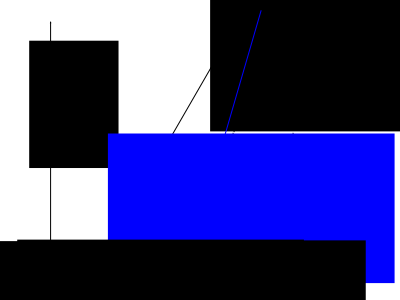
\includegraphics{img/splines.pdf}
    \caption{Linear combination of aborted powers of order 2}
    \label{img:splines}
  \end{center}
\end{figure}

The basis $B$ is not appropriate to represent a spline $s \in S_{k,\Delta}$, because
\begin{itemize}
  \item the support of monomials $t^i$ is entire $\mathbb R$. $\mathbb R \setminus \Set{0}$.
  \item for points with $t_i \approx t_{i+1}$, the aborted powers are \emph{almost} linear dependent.
    \[ s(t) = \sum_{i=0}^{k-1} a_i t^i + \sum_{i=1}^{n-1} c_i (t - t_i)_+^{k-1} \]
\end{itemize}

\index{B-Splines}
\begin{definition}
  \label{definition:4-21}
  Let $\tau_1 \leq \tau_2 \leq \dots \leq \tau_d$ be an arbitrary sequence of points.
  Then the B-splines $N_{i,k}(t)$ of order $k$ for $k = 1, \dots, d$ and $i = 1, \dots, d-k$
  are recursively defined by
  \[
    N_{i,1}(t) \coloneqq \chi_{[\tau_i,\tau_{i+1})}(t) = \begin{cases}
      1 & \text{ if } \tau_i \leq t < \tau_{i+1} \\
      0 & \text{ else}
    \end{cases}
  \] \[
    N_{i,k}(t) = \frac{t - \tau_i}{\tau_{i+k-1} - \tau_i} N_{i,k-1}(t) + \frac{\tau_{i+k} - t}{\tau_{i+k} - \tau_{i+1}} N_{i+1,k-1}(t)
  \]
\end{definition}

\begin{Remark}
  The characteristic function $\chi$ vanishes for collapsing points.
  In the recursion, expressions of form $\frac00 \coloneqq 0$ are defined.
  Thus, B-splines are also given for collapsing points.
\end{Remark}

\begin{example}[$k=2$]
  \begin{align*}
    N_{i,2}(t) &= \frac{t - \tau_i}{\tau_{i+1} - \tau_i} N_{i,1}(t) + \frac{\tau_{i+2} - t}{\tau_{i+2} - \tau_{i+1}} N_{i+1,1}(t) \\
      &= \frac{t - \tau_i}{\tau_{i+1} - \tau_i} \chi_{[\tau_i,\tau_{i+1})} + \frac{\tau_{i+2} - t}{\tau_{i+2} - \tau_{i+1}} \chi_{[\tau_{i+1},\tau_{i+2})}
  \end{align*}
\end{example}

\begin{figure}[!ht]
  \begin{center}
    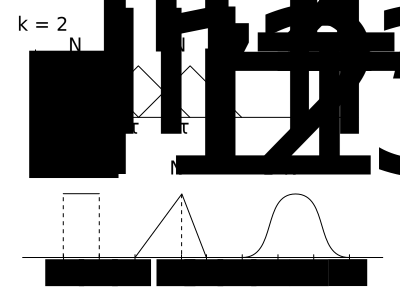
\includegraphics{img/bsplines.pdf}
    \caption{B-splines of order $k = 2$ or $k = 1, 2, 3$}
  \end{center}
\end{figure}

For the B-splines, as defined above, the following properties hold:
\index{Local support}
\begin{enumerate}
  \item $\operatorname{supp}(N_{i,k}) \subset [\tau_i, \tau_{i+k}]$ (\emph{local support})
  \item $N_{i,k}(t) \geq 0 \forall t \in \mathbb R$ (non-negative)
  \item $N_{i,k}$ is a piecewise polynomials of degree $k-1$ with respect to intervals $[\tau_i, \tau_{i+1}]$.
\end{enumerate}

\dateref{2018/11/27}

Alternatively we can write B-splines as divided differences for the aborted power $f_t(s) = (s - t)_t^{k-1}$.

\begin{lemma}
  \label{lemma:b-spline}
  If $\tau_i < \tau_{i+k}$, then B-spline $N_{i,k}$ satisfies
  \[ N_{i,k}(t) = (\tau_{i+k} - \tau_i) \cdot \begin{bmatrix} \tau_i & \dots & \tau_{i+k} \end{bmatrix} (\cdot -t)_{+}^{k-1} \]
  where $\cdot$ in $(\cdot -t)_{+}^{k-1}$ denotes a parameter (yielding a function as defined in Remark~\ref{plus-notation}). The specific value of $\,\cdot$\, becomes irrelevant.

  If $\tau_j$ is a point with multiplicity $M$, hence $\tau_j = \tau_{j+M-1}$, then $N_{i,k}$ at point $\tau_j$ is a least $(k-1-n)$ times differentiable. For $M < k-1$. For $N_{i,k}$, it is true that
  \[ N_{i,k}'(t) = (k-1)\left(\frac{N_{i,k-1}(t)}{\tau_{i+k-1} - \tau_i} - \frac{N_{i+1,k}(t)}{\tau_{i+k} - \tau_{i+1}}\right) \]
\end{lemma}

\noproof{lemma:b-spline}

\emph{Goal:} Characterize $\rho_{k}$ by B-splines\dots

Therefore introduce \emph{extended points sequence} $T = \Set{t_j}_{j=1}^{\alpha+k}$ where the boundary points $a = t_0$ and $b = t_n$ are each counted $k$ times.
\[ \triangle: a = t_0 < t_1 < \dots < t_n = b \]
\[ T: \tau_1 = \dots = t_k < t_{k+1} < \dots < \tau_{d+1} = \dots = \tau_{d+k} = b \]
with $d = n-1+k = \dim(S_{k,0})$.

It can be shown that the $B$-splines $N_{i,k}$, for $i = 1, \dots, k$, corresponding to extended points $T$ create a basis of $S_{k,\delta}$.

\begin{example}
  \[ t_0 < t_1 < t_2 < t_3 \]
  \[ \tau_1 = \tau_2 = t_0 \qquad \tau_3 = t_1 \qquad \tau_4 = t_2 \qquad \tau_5 = \tau_6 = t_4 \]
  \[ N_{1,2} = \frac{\tau_3 - t}{\tau_3 - \tau_2} \cdot X_{[\tau_2, \tau_3]} \]


  TODO image splines

  Thus, every spline $s \in S_{k, \delta}$ has a unique representation as linear representation $s = \sum_{i=1}^d \alpha_i N_{i,k}$. $\alpha_i$ is called \emph{De-Boor points} of $s$.

  Special case $k=2$ (interpolation of $f$: $\alpha_i = f(t_{i-1})$.
\end{example}


\section{Computational quadrature}
\label{sec:5}

\emph{Goal:} Numerical computation (approximation of Riemann integral)
\[ I(f) \coloneqq I_a^b(f) = \int_a^b f \, dt \]
with some piecewise continuous function $f$.

Numerical integration is primarily solved for solving the initial value problem $y'(t) = f(t)$, $y(a) = 0$, $t \in [a, b] \implies y(b) = I(f)$.

\subsection{Quadrature formulas}
\label{sec:5-1}

Assume $b > a$. The definite integral $I_a^b: C[a, b] \to \mathbb R$ with $f \mapsto \int_a^b f \, dt$ is a \emph{positive} linear form, thus
\begin{enumerate}
  \item $I$ is linear, $I(\alpha f + \beta g) = \alpha I(f) + \beta I(g)$
  \item $I$ is positive: $f \geq 0 \implies I(f) \geq 0$
  \item \emph{additivity:} $I_a^b(f) = I_a^c(f) + I_c^b(f)$
\end{enumerate}

\emph{Question:} Condition of $I$?
  We choose the $L^1$-norm:
  \[ \Abs{f}_1 \coloneqq \int_a^b \Abs{f(t)} \, dt = I_a^b(\Abs{f}) \]

\begin{lemma}
  \label{lemma:5-1}
  The absolute and relative condition of quadrature problem ($I, f$),
  $I(f) = \int_a^b f$ with respect to $L^1$-norm $\Abs{\cdot}_1: \kappa_{\text{abs}} = 1, \kappa_{\text{rel}} = \frac{I(\Abs{f})}{\Abs{I(f)}}$
\end{lemma}

\begin{proof}
  We investigate: $\Norm{I(\tilde f) - I(f)} \dot\leq \kappa_{\text{abs}} \cdot \Abs{\tilde f - f}$.

  For every deviation $S_f \in C[a, b]$ we get:
  \begin{align*}
    \Norm{I_a^b(f + S_f) - I(f)}_1
      &= \Norm{I(f + S_f - f)}_1 = \Norm{I(S_f)}_1 = \Abs{\int_a^b S_f} \\
      &\leq \int_a^b \Abs{S_f} = \Norm{I(\Abs{S_f})} \implies \kappa_{\text{abs}} = 1
  \end{align*}
  Especially for positive deviation, we get equality.
  We investigate:
  \[ \frac{\Norm{I(\tilde f) - I(f)}}{\Norm{I(f)}} \dot\leq \kappa_{\text{rel}} \frac{\Norm{\tilde f - f}}{\Norm{f}} \]
  We know:
  \[ \frac{\Norm{I(\tilde f) - I(f)}}{\Norm{I(f)}} \dot\leq 1 \cdot \frac{\Norm{\tilde f - f}}{\Norm{I(f)}} \cdot \frac{\overbrace{\Abs{f}}^{= I(\Abs{f})}}{\Abs{f}} \implies \kappa_{\text{rel}} = \frac{I(\Abs{f})}{\Abs{I(f)}} \]
\end{proof}

\begin{Remark}
  For strongly oscillating functions, relative conditions can become very large.
\end{Remark}

\emph{Goal:}
  Numerical quadrature shall be used to create a positive linear form on $C[a, b]$. \[ \hat I: f \mapsto \hat I(f) \]
  We want to create $\hat I$ und want to approximate $I$ in the best possible way $\implies I(f) \approx \hat I(f)$.

  TODO image Riemann

  $\to$ Riemann sums or trapezoidal sums

\begin{example}[Trapezoidal sums]
  Decompose $[a, b]$ in $n$ subintervals $[t_{i-1}, t_i]$. $h_i \coloneqq t_i - t_{i-1}$.

  Approximate $\int f$ by the sum of trapezoidal areas $T^{(n)} = \sum_{i=1}^n T^{(i)}$, $T^{(i)} = \frac{h_i}{2} (f(t_{i-1}) + f(t_i))$
  Thus, $T^{(n)}$ is a positive linear form.

  Now we consider the Riemann lower/upper sum: $R_u^{(n)} \leq T^{(n)} \leq R_0^{(n)}$.

  For $n \to \infty$ and $f$ continuous, $R_u$ and $R_o$ converge, hence $T$ converges as well.
\end{example}

\index{Quadrature formula}
\begin{definition}
  \label{definition:5-3}
  $\hat I$ is called \emph{quadrature formula} for computation of $I(f)$ if:
  $\hat I(f) = (b - a) \cdot \sum_{i=0}^{n} \lambda_i f(t_i)$ with points
  $t_0, \dots, t_n$ and weights $\lambda_0, \dots, \lambda_n: \sum \lambda_i = 1$.
\end{definition}

Be aware that condition $\sum \lambda_i = 1$ requires that constant functions are integrated accurately.

Furthermore: $\hat I$ is positive iff $\lambda_i \geq 0 \forall i$.

Using $\sum \Abs{\lambda_i} \geq 1$ we can specify how much the positivity property is violated.

\subsection{Newton-Cotes formula}
\label{sec:5-2}

\emph{Idea:} Approximate $f$ by some piecewise linear function, that is integrated accurately, thus $\hat I(f) = I(\hat f)$.

For $t_0, \dots, t_n$ use the interpolation polynomial $\hat f(t) = P(f \, \mid \, t_0, \dots, t_n) = \sum_{i=0}^n f(t_i) \cdot L_{i,n}(t)$ with Lagrange polynomials $L_{i,n}(t) = \prod_{\substack{j \neq i \\ j=0}} \frac{t - t_j}{t_i - t_j}$.

This gives the quadrature formulas $\hat I(f) = I(P(f \,\mid\, t_0 \dots t_n)) = (b - a) \cdot \sum \lambda_{i,n} f(t_i)$ with $\lambda_{i,n} = \frac{1}{(b-a)} \cdot \int_a^b L_{i,n}(t) \, dt$.

\begin{lemma}
  \label{lemma:5-4}
  For $n+1$ pairwise different points $t_0, \dots, t_n$ there is exactly one quadrature formula $\hat I(f) = (b - a) \sum \lambda_i f(t_i)$, that are exact for all $P \in \mathcal P_n$.
\end{lemma}

\begin{proof}
  Let $L_{i,n}$ be Lagrange polynomials for points $t_i$. Necessarily,
  \[ \hat I(L_{i,n}) = I(L_{i,n}) = (b-a) \cdot \sum \lambda_j \underbrace{L_{i,n}(t_j)}_{= \delta_{i,j}} = (b-a) \cdot \lambda_i \cdot L_{i,n}(t_j) \]
  \[ \implies \lambda_i = \frac{I(L_{i,n})}{b-a} \]
\end{proof}

For equivalent points $h_i = h = \frac{b-a}{n}$ and $t_i = a + i \cdot n$ we retrieve the \emph{Newton-Cotes formulas}.

The corresponding Newton-Cotes weights are given by
\[ \lambda_{i,n} = \frac{1}{b - a} \int_a^b \prod_{\substack{j = 0 \\ j \neq i}}^n \frac{t - t_j}{t_i - t_j} = \frac 1n \int_0^n \prod \frac{s - j}{i - j} \, ds \]
Substitute $s = \frac{t - a}{h}$.  The weights are independent of interval boundaries. They only must be computed once.

\begin{table}[!ht]
  \begin{center}
    \begin{tabular}{cccc}
      $n$ & $\lambda_{0,n} \dots \lambda_{n,n}$   & Error & $\tau \in [a,b]$ \\
    \hline
      $1$ & $\frac12, \frac12$                    & $\frac{h^3}{12} f''(\tau)$                     & trapezoidal rule \\
      $2$ & $\frac16, \frac46, \frac16$           & $\frac{h^5}{90} f^{(4)}(\tau)$                 & Simpson rule, \dt{Keplersche Faßregel} \\
      $3$ & $\frac18, \frac38, \frac38, \frac18$  & $\frac{3 \cdot h^5}{80} \cdot f^{(4)}(\tau)$   & Newton's $\frac38$ rule \\
      $4$ & $\frac7{90}, \frac{32}{90}, \frac{12}{90}, \frac{32}{90}, \frac{7}{90}$ & $\frac{8 \cdot h^7}{945} \cdot f^{(6)}(\tau)$ & Milne rule
    \end{tabular}
    \caption{Newton-Cotes weights $\lambda_{i,n}$ for $n = 1, \dots, 4$}
  \end{center}
\end{table}

For orders $1$ to $7$, the weights are positive. For $n = 8$ and higher, negative weights can occur. This is mostly irrelevant in practice.

\begin{lemma}
  \label{lemma:5-5}
  For $g, h \in C[a, b]$, $g \geq 0$ or $g \leq 0$, $\forall t \in [a, b]$ we have:
  \[ \int g \cdot h = h(\tau) \cdot \int g \, dt \]
  for some $\tau \in [a, b]$.
\end{lemma}

\begin{proof}
  Without loss of generality $g \geq 0$
  \[ \min_{t \in [a,b]} h(t) \cdot \int_a^b g(s) \, ds \leq \int h \cdot g \leq \max h(t) \int g \]
  \[ F(t) \coloneqq \int h \cdot g \, ds - h(t) \int g \, ds \]
  \[ F(a) \geq 0, F(b) \leq 0 \]
  \[ \text{IVT } \implies \exists t: F(t) = 0 \implies \int h \cdot g = h(t) \cdot \int g \]
\end{proof}

\begin{Lemma}
  Let $f \in \mathcal C^2[a, b]$.
  For the approximation error the trapezoidal rule $T = \frac{b-a}{2} (f(a) + f(b))$ with $h = b - a$ we have:
  \[ T = \int f = \frac{h^3}{12} f''(\tau) \]
  for some $\tau \in [a, b]$.
\end{Lemma}

\dateref{2018/11/29}

\begin{lemma}
  \label{lemma:5-6}
  The map, given by $n$-th divided difference of a function $f \in \mathcal C^1([a, b])$, $g: \mathbb R^{n + 1} \to \mathbb R$ with $g(t_0, \dots, t_n) = [t_0, \dots, t_n] f$ is continuous in its arguments $t_i$. Furthermore there exists some $\xi \in [t_0, t_n]$ for all points $t_0 \leq \dots \leq t_n$ such that
  \[ [t_0, \dots, t_n] f = \frac{f^{(n)}(\xi)}{n!} \]
\end{lemma}

\begin{lemma}
  \label{lemma:5-7}
  Let $f \in \mathcal C^2([a,b])$. The approximation error of the trapezoidal rule $T = \frac{b - a}{2} (f(a) - f(b))$ with step size $h \coloneqq b - a$ it holds that
  \[ T - \int_a^b f \, dt = \frac{h^3}{12} f''(\tau) \]
  for some $\tau \in [a,b]$.
\end{lemma}

\begin{proof}
  By Theorem~\ref{theorem:4-10}, we know that
  \[ f(t) = P(t) + [a, b, t] f \cdot \underbrace{(t - a)}_{\geq 0} \underbrace{(t - b)}_{\geq 0} \]
  and by Lemma~\ref{lemma:5-6} furthermore
  \[ [a,b,t] f = \frac{f^k(\xi)}{2} \]
  for some $\chi \in [a,b]$ depending on $t$.
  For the square rule (see extended Mean Value Theorem), this means
  \begin{align*}
    \int_a^b f \, dt
      &= \int_a^b P(t) \, dt + \int_a^b [a, b, t] f \cdot \underbrace{(t - a)}_{\geq 0} \underbrace{(t - b)}_{\leq 0} \\
      &= T + \frac{f''(\tau)}{2} \underbrace{\int_a^b (t - a) (t - b)}_{= -\frac{(b - a)^3}{6} \text{ for some } \tau \in [a,b]}
  \end{align*}
  for some $\tau \in [a,b]$. Therefore, in total,
  \[ T = \int_a^b f \, dt = \frac{h^3}{12} f''(\tau) \]
\end{proof}

\begin{lemma}[Simpson's rule, \dt{Keplersche Fassregel}]
  \label{lemma:5-8}
  \[ S = \frac{b - a}{6} (f(a) + 4f\left(\frac{a + b}{2}\right) + f(b)) \]
  is exact for polynomials $Q \in \mathcal P_3$.
  For $f \in \mathcal C^4([a,b])$, the approximation error can be expressed with step size $\frac{b - a}{2}$ as
  \[ S = \int_a^b f \, dt = \frac{f^{(4)}(\tau)}{90} h^5 \]
  for some $\tau \in [a,b]$.
\end{lemma}

\begin{proof}
  Let $Q \in \mathcal P_3$. By Theorem~\ref{theorem:4-10}, it follows by $P(Q \,\mid\, a, \frac{a+b}{2}, b)$
  \[ Q(t) = P(t) + \gamma \underbrace{\gamma (t - a) \left(t - \frac{a+b}{2}\right) (t - b)}_{w_3(t)} \]
  with some constant $\gamma = \frac{Q'''(\xi(t))}{6} \in \mathbb R$. For the integral, we have:
  \[ \int_a^b Q(t) \, dt = \int_a^b P(t) \, dt + \gamma \underbrace{\int_a^b w_3(t) \, dt}_{= 0} \]
  provides the first statement.

  For $f \in \mathcal C^4([a, b])$, we create the Hermite interpolant $Q = P_4(f \,\mid\, a, \frac{a+b}{2}, \frac{a+b}{2}, b)$.
  By the remainder term formula, we get:
  \[ f(t) = Q(t) + [a, \frac{a+b}{2}, \frac{a+b}{2}, b, t] f \underbrace{(t - a) \left(t - \frac{a + b}{2}\right)^2 (t - b)}_{= w_4(t)} \]
\end{proof}

\dateref{2018/12/04}

\subsection{Gauss–Christoffel Quadrature Formulas}
\label{ch:5-3}

Our goal is to compute \enquote{optimal} points $t_i$ and weights $\lambda_i$ such that
$I(P) = \hat{I}(P)$ for $P \in \mathcal P_N$ with $N \to \max$. Now we consider the general integral of form $I(f) \coloneqq \int_a^b w(t) f(t) \, dt$ with some positive weight functions $w(t) > 0$, $t \in (a,b)$.
We assume that norms $\Norm{P} = \sqrt{\IP{P}{P}_w} = \left(\int_a^b w(t) P(t) \, dt\right)^{\frac12} < \infty$ are well-defined for all $P \in \mathcal P_k$ and all $k \in \mathbb N$.
For $a = -\infty$ and $b = \infty$, we require that moments $\mu_k$ are bounded:
\[ \mu_k \coloneqq \int_{-\infty}^\infty t^k \cdot w(t) \, dt \]

\begin{remark}
  TODO There must be number 5.9 somewhere here.
\end{remark}

For the condition analysis, use weighted $L^1$-norm
\[ \Norm{f}_{1,W} = \int_a^b w(t) f(t) \, dt \eqqcolon I(\Abs{f}) \]
This is the analogous result for Lemma~\ref{lemma:5-1}.

Typical weight functions are:
\begin{itemize}
  \item $w(t) = 1$ on $[-1,1]$
  \item $w(t) = \frac{1}{\sqrt{1 - t^2}}$ on $[-1,1]$
  \item $w(t) = e^{-t}$ on $[0,\infty)$
  \item $w(t) = e^{-t^2}$ on $(-\infty, \infty)$
\end{itemize}

\emph{Construction:}
For given $n$, construct quadratic formulas of form $\hat{I}_n(f) \coloneqq \sum_{i=0}^n \lambda_{i,n} f(\tau_{i,n})$ with $n+1$ points $\tau_{0,n},\dots,\tau_{n,n}$ and weights $\lambda_{0,n}, \dots, \lambda_{n,n}$ such that $\hat{I}_n(P) = I(P)$ for all $P \in \mathcal P_N$.
We have $2n + 2$ free parameters for a polynomial with $N+1$ coefficients. We guess $N \leq 2n+1$ (but consider the non-linearity of the problem!). It is possible to prove that $N \leq 2n+1$.

\begin{lemma}
  \label{lemma:5-10}
  If $\hat{I}_n$ is exact for all polynomials $P \in \mathcal P_{2n+1}$, then $P_{n+1}$ is defined by \[ P_{n+1} \coloneqq (t - \tau_{0,n}) \dots (t - \tau_{n,n}) \]
  orthogonal to arbitrary $P_j \in \mathcal P_j$, $j < n + 1$ with respect to the scalar product weighted by $w$.
\end{lemma}

\begin{proof}
  For $P_j \in \mathcal P_j$ with $j < n+1$, we have $P_{n+1} P_j \in \mathcal P_{2n+1}$.
  Thus,
  \begin{align*}
    \IP{P_j}{P_{n+1}} &= \int_a^b w(t) P_j(t) P_{n+1}(t) \, dt \\
      &= \hat{I}_n(P_j P_{n+1}) = \sum_{i=0}^n \lambda_{i,n} P_j(\tau_{i,n}) \underbrace{P_{n+1}(\tau_{i,n})}_{=0} = 0
  \end{align*}
\end{proof}

\begin{thm}
  \label{theorem:5-11}
  For every weighted scalar product ${\IP fg}_w \coloneqq \int_a^b w(t) f(t) g(t) \, dt$ there exists a uniquely determined orthogonal polynomial $P_k \in \mathcal P_k$ with leading coefficient $1$. They satisfy the so-called \emph{three-term recursion}
  \[ P_k(t) = (t + a_k) P_{k-1}(t) + b_k P_{k-2}(t) \qquad \text{ for } k = 1,2,\dots \]
  with the initial values $P_{-1} = 0$, $P_0 = 1$ and the coefficients
  \[
    a_k = -\frac{\IP{t P_{k-1}}{P_{k-1}}_w}{\IP{P_{k-1}}{P_{k-1}}_w} \qquad
    b_k = -\frac{\IP{P_{k-1}}{P_{k-1}}_w}{\IP{P_{k-2}}{P_{k-2}}_w}
  \]
\end{thm}

\begin{proof}
  For $k = 0$, there exists a polynomial $p_0 \equiv 1 \in \mathcal P_0$ with leading coefficient $1$.
  Now let $P_0, \dots, P_{k-1}$ be pairwise orthogonal polynomials $P_j \in \mathcal P_j$ of degree $j$ with leading coefficient $1$. Let $P_k \in \mathcal P_k$ be a normed polynomial of degree $k$. The $P_k - t P_{k-1} \in \mathcal P_{k-1}$ and because $P_0, \dots, P_{k-1}$ define an orthonormal basis of $\mathcal P_{k-1}$, we have
  \[ P_k - t P_{k-1} = \sum_{j=0}^{k-1} c_j P_j \qquad c_j = \frac{\IP{P_k - t P_{k-1}}{P_j}_w}{\IP{P_j}{P_j}_W} \]
  By the requirement $\IP{P_k}{P_j}_w = 0 \forall j = 0, \dots, k-1$, we get
  \[ c_j = -\frac{\IP{t P_{k-1}}{P_j}_w}{\IP{P_j}{P_j}_w} = -\frac{\IP{P_{k-1}}{tP_j}}{\IP{P_j}{P_j}} \]
  This implies $c_0 = \dots = c_{k-3} = 0$ (orthogonality of $P_{k-1}$ to $P_j$, $j < k-1$).
  Furthermore,
  \begin{align*}
    c_{k-1} &= -\frac{\IP{t P_{k-1}}{P_{k-1}}_v}{\IP{P_{k-1}}{P_{k-1}}_w} \\
    c_{k-2} &= -\frac{\IP{P_{k-1}}{t P_{k-2}}_w}{\IP{P_{k-2}}{P_{k-2}}_w}
            = -\frac{\IP{P_{k-1}}{P_{k-1}}_w}{\IP{P_{k-2}}{P_{k-2}}_w}
  \end{align*}
  (because $t P_{k-2} \in \mathcal P_{k-1}$ and $P_0, \dots, P_{k-1}$ orthonormal basis).
  $P_k$ follows:
  \[ P_k = (t + C_{k-1}) P_{k-1} + c_{k-2} P_{k-2} = (t + a_k) P_{k-1} + b_k P_{k-2} \]
\end{proof}

By the two previous results, we conclude that the points must be the roots of the uniquely determined orthogonal polynomial $P_{n+1}$ (for appropriate weight $w$). To integrate polynomials of degree $n$ exactly, we can use the fact that the weights satisfy
\[ \lambda_{i,n} = \frac{1}{b - a} \int_a^b L_{i,n}(t) \, dt \]
with Lagrange polynomials $L_{i,n}$.

\begin{lemma}
  \label{lemma:5-12}
  Let $\tau_{0,n}, \dots, \tau_{n,n}$ be the roots of the $(n+1)$-th orthogonal polynomial $P_{n+1}$. Then every quadrature formula $\hat{I}_n(f) = \sum_{i=0}^n \lambda_i f(\tau_{i,n})$ satisfies:
  \[ \hat{I}_n \text{ is exact on } \mathcal P_n \iff \hat{I}_n \text{ exact on } \mathcal P_{2n+1} \]
\end{lemma}

\begin{proof}
  Direction $\impliedby$ is immediate. Direction $\implies$:

  Let $\hat{I}_n$ be exact on $\mathcal P_n$ and $P \in \mathcal P_{2n+1}$.
  Then polynomials $Q, R \in \mathcal P_n$ exist such that $P = QP_{n+1} + R$. Thus, it follows that
  \[ \int_a^b w \, P = \int_a^b w Q P_{n+1} + \int_a^b R w = 0 + \hat{I}_n(R) \]
  Additionally, it holds that
  \[ I(P) = \int_a^b w P = \hat{I}_n(R) \]
  \[ = \sum_{i=0}^n \lambda_{i,n} R(\tau_{i,n}) = \sum_{i=0}^n \lambda_{i,n}\left(R(\tau_{i,n}) + (P_{n+1} \cdot Q)(\tau_{i,n})\right) = \hat{I}(P) \]
\end{proof}

\begin{thm}
  \label{theorem:5-13}
  There exists uniquely determined points $\tau_{0,n}, \dots, \tau_{n,n}$ and weights $\lambda_{0,n}, \dots, \lambda_{n,n}$ such that for the quadrature formula
  \[ \hat{I}_n(f) = \sum_{i=0}^n \lambda_{i,n} \cdot f(\tau_{i,n}) \]
  it holds that
  \[ \hat{I}_n(P) = \int_a^b wP \forall P \in \mathcal P_{2n+1} \]
  The points $\tau_{i,n}$ are the roots of the $(n+1)$-th orthogonal polynomial $P_{n+1}$ (with leading coefficient $1$) with respect to weight function $w$ and the weights are
  \[ \lambda_{i,n} \coloneqq \frac{1}{b-a} \int_a^b L_{i,n}(t) \, dt \]
  with Lagrange polynomials $L_{i,n}(\tau_{j,n}) = \delta_{i,j}$. Furthermore it holds that $\lambda_{i,n} > 0$, hence $\hat{I}_n$ is the positive linear form and
  \[ \lambda_{i,n} = \frac{1}{P_{n+1}'(\tau_{i,n}) P_n(\tau_{i,n})} \IP{P_n}{P_n}_w \]
\end{thm}

\begin{proof}
  Show: positivity / representation of $\lambda_{i,n}$

  Choose $Q \in \mathcal P_{2n+1}$ such that $Q(\tau_{i,n}) = 0$ for $i \neq k$ and $Q(\tau_{k,n}) \neq 0$ for some point $\tau_{k,n}$. Then
  \[ \int_a^b w Q = \lambda_{k,n} Q(\tau_{k,n}) \]
  \[ \implies \lambda_{k,n} = \frac{1}{Q(\tau_{k,n})} \int_a^b wQ \]
  Especially, this holds for
  \[ Q(t) \coloneqq \left(\frac{P_{n+1}(t)}{(t - \tau_{k,n})}\right)^2 = \left(\prod_{\substack{i = 0 \\ l \neq k}}^n (t - \tau_{i,n})\right)^2 \]
  It holds that $Q \in \mathcal P_{2n}$ and $Q(\tau_{k,n}) = P_{n+1}'(\tau_{k,n})^2$.
  Thus we get
  \[ \lambda_{k,n} = \frac{1}{Q(\tau_{k,n})} \int_a^b wQ = \int_a^b w \left(\frac{P_{n+1}(t)}{P'_{n+1}(\tau_{k,n}) (t - \tau_{k,n})}\right)^2 \, dt > 0 \]
  and therefore the positivity of the weights. For the representation of the weights, we let
  \[ Q(t) \coloneqq \frac{P_{n+1}(t)}{t - \tau_{k,n}} P_n(t) \]
  Furthermore $Q \in \mathcal P_{2n}$ and it follows that
  \[ \lambda_{k,n} = \frac{1}{P'_{n+1}(\tau_{k,n}) P_n(\tau_{k,n})} \int_a^b w(t) \frac{P_{n+1}(t)}{t - \tau_{k,n}} P_n(t) \, dt \]
  The leading coefficient of $\frac{P_{n+1}(t)}{t - \tau_{k,n}}$ is $1$, such that
  \[ \frac{P_{n+1}(t)}{t - \tau_{k,n}} = P_n(t) + Q_{n-1}(t) \text{ for some } Q_{n-1} \in \mathcal P_{n-1} \]
  Because $Q_{n-1}$ is orthogonal to $P_n$,
  \[ \lambda_{k,n} = \frac{1}{P'_{n+1}(\tau_{k,n}) P_n(\tau_{k,n})} \IP{P_n}{P_n}_w \]
\end{proof}

\begin{Remark}
  The quadrature formulas $\hat{I}_n$ resulting from the theorem are called Gauss-Christoffel formulas of the weight function $w$.
\end{Remark}

\paragraph{Error estimate}
\begin{thm}
  \label{theorem:5-14}
  The approximation error of the Gauss-Christoffel quadrature can be expressed for every function $f \in \mathcal C^{2n+2}([a,b])$ as
  \[ \int_a^b w f \, dt - \hat{I}_n(f) = \frac{f^{(2n+2)}(\tau)}{(2n+2)!} \IP{P_{n+1}}{P_{n+1}}_w \text{ for some } \tau \in [a,b] \]
\end{thm}

\begin{proof}
  Let $P \in \mathcal P_{2n+1}$ be the Hermitian interpolant of $f$ at $2n+2$ points $\tau_{0,n}, \tau_{0,n}, \dots, \tau_{n,n} \tau_{n,n}$. Then
  \[ f(t) = P(t) + [\tau_{0,n}, \tau_{0,n}, \dots, \tau_{n,n}, \tau_{n,n}, t] f \underbrace{(t - \tau_{0,n})^2 \dots (t - \tau_{n,n})^2}_{(P_{n+1}(t))^2 \geq 0} \]
  Because $\hat{I}_n$ integrates the function $P$ exactly, we get
  \begin{align*}
    \int_a^b w f \, dt
      &= \int_a^b w P \, dt + \frac{f^{(2n+2)}(\tau)}{(2n+2)!} \int_a^b w P_{n+1}^2 \, dt \\
      &= \sum_{i=0}^n \lambda_{i,n} P(\tau_{i,n}) + \frac{f^{(2n+2)}(\tau)}{(2n+2)!} \IP{P_{n+1}}{P_{n+1}}_w \\
    \intertext{by Hermitian interpolant}
      &= \sum_{i=0}^n \lambda_{i,n} f(\tau_{i,n}) + \frac{f^{(2n+2)}(\tau)}{(2n+2)!} \IP{P_{n+1}}{P_{n+1}}_w \\
      &= \hat{I}_n(f) + \frac{f^{(2n+2)}(\tau)}{(2n+2)!} \IP{P_{n+1}}{P_{n+1}}_w
  \end{align*}
\end{proof}

\begin{example}[Gauss-Chebyshev quadrature]
  For $[-1,1]$, $w(t) = \frac{1}{\sqrt{1 - t^2}}$ and the Chebyshev polynomials $T_k$ it holds that
  \[
    \int_{-1}^1 \frac{T_k(t) T_j(t)}{\sqrt{1 - t^2}} \, dt
    = \begin{cases}
      \pi & \text{ if } k = j = 0 \\
      \pi/2 & \text{ if } k = j > 0 \\
      0 & \text{ if } k \neq j
    \end{cases}
  \]

  Thus $P_n(t) = 2^{1-n} T_n(t)$ are the orthogonal polynomials with leading coefficient 1. The roots of $P_{n+1}$ are the Chebyshev points
  \[ \tau_{i,n} = \cos\left(\frac{2i+1}{2n+2} \pi\right) \quad i = 0,\dots,n \]
  For $n > 0$, we get the weights
  \[ \lambda_{i,n} = \frac{1}{2^{-n} T_{k+1}'(\tau_{i,n}) 2^{1-n} T_n(\tau_{i,n})} \int_{-1}^1 \frac{2^{2 - 2n} T_n^2}{\sqrt{1 - t^2}} \, dt = \frac{2\pi/2}{T'_{n+1}(\tau_{i,n}) T_n(\tau_{i,n})} = \frac{\pi}{n+1} \]

  Implies the Gauss-Chebyshev quadrature of form
  \[ \hat{I}_n(f) = \frac{\pi}{n+1} \sum_{i=0}^n f(\tau_{i,n}) \text{ with } \tau_{i,n} = \cos\left(\frac{2i+1}{2n+2} \pi\right) \]
  with approximation error
  \[ \int_{-1}^1 \frac{f(t)}{\sqrt{1 - t^2}} \, dt - \hat{I}_n(f) = \frac{\pi}{2^{2n+1} (2n+2)!} f^{(2n+2)}(\tau) \text{ for } \tau \in [-1,1] \]
\end{example}

\dateref{2018/12/06}

Common orthogonal systems are:
\begin{enumerate}
  \item Chebyshev polynomials $T_n$ for $w(t) = \frac{1}{\sqrt{1 - t^2}}$ on $[-1, 1]$
  \item Laguerre polynomials $L_n$ for $w(t) = w^{-t}$ on $[0, \infty)$
  \item Hermitian polynomials $H_n$ for $w(t) = e^{-t^2}$ on $(-\infty, \infty)$
  \item Legendre polynomials $P_n$ for $w(t) = 1$ on $[-1, 1]$
\end{enumerate}

\paragraph{Computation of roots and weights}

Disadvantages of Gauss-Christoffel quadrature:
\begin{enumerate}
  \item coefficients/points depend on the integration interval
  \item for every $n$ we retrieve different coefficients/points
\end{enumerate}

The first disadvantage can be fixed by the affine linear transformation
\[ t = \frac{b - a}{2} x + \frac{a + b}{2} \]
\[ \implies I(f) = \int_a^b f(t) \, dt = \frac{b - a}{2} \int_{-1}^1 \underbrace{f\left(\frac{b - a}{2} x + \frac{a + b}{2}\right)}_{\tilde f(x)} \, dx \]
\[ \implies \hat{I}(f) = \frac{b - a}{2} \sum_{i=0}^n \lambda_{i,n} f\left(\frac{b - a}{2} \tau_{i,n} + \frac{a + b}{2}\right) \]
If we want to approximate an integral $\int_a^b f(t) \, dt$, we can write it as
\[ \int_a^b \underbrace{\frac{f(t)}{w(t)}}_{\tilde f(t)} \cdot w(t) \, dt \]
In practice, points $\tau_{i,n}$ and weights $\lambda_{i,n}$ will be determined for the orthogonal polynomials based on the three-term recursion.

By Theorem~\ref{theorem:5-11}, we know that
\[ P_k(t) = (t - \beta_k) P_{k-1}(t) - \gamma_k^2 P_{k-2}(t) \]
\[ \text{ with } \qquad \beta_k = \frac{\IP{t P_{k-1}}{P_{k-1}}_w}{\IP{P_{k-1}}{P_{k-1}}_w} \qquad \gamma_k^2 = \frac{\IP{P_{k-1}}{P_{k-1}}_w}{\IP{P_{k-2}}{P_{k-2}}_w} \]
If the orthogonal polynomials are given by this recursion, we can define the linear equation system $T_p = t p + r$ with
\[
  T \coloneqq \begin{bmatrix}
    \beta_1    & 1       &            &                & \\
    \gamma_2^2 & \beta_2 & 1          &                & \\
               & \ddots  & \ddots     & \ddots         & \\
               &         & \gamma_n^2 & \beta_n        & 1 \\
               &         &            & \gamma_{n+1}^2 & \beta_{n+1}
  \end{bmatrix}
  \qquad p \coloneqq \begin{bmatrix} P_0(t) \\ \vdots \\ P_n(t) \end{bmatrix}
  \qquad r \coloneqq \begin{bmatrix} 0 \\ \vdots \\ 0 \\ -P_{n+1}(t) \end{bmatrix}
\]
Then it holds that $P_{n+1}(t) = 0 \iff T_p = t_p$, so the roots of $P_{n+1}$ are the eigenvalues of $T$ and for every eigenvalue $\tau$, we have a corresponding eigenvector $P(\tau)$.

All roots are real.

\emph{Question:} Can we write it as symmetric eigenvalue problem?

\emph{Trial:} Scaling of eigenvalue problem with some diagonal matrix $D = \diag(d_0, \dots, d_n)$ such that $\hat{T} \hat{p} = t \hat{p}$ with $\hat{p} = Dp$ and $\hat{T} = DTD^{-1}$.

For the orthogonal scaling applied to $A \in \mathbb R^{(n+1) \times (n+1)}$ it is true that $A \mapsto \hat{A} \coloneqq D A D^{-1}$. $\hat{a_{ij}} = \frac{di}{dj} a_{ij}$.

For symmetry of $\hat{T}$ we require that
\[ \gamma^2_{i+1} \frac{d_i}{d_{i-1}} = \frac{d_{i-1}}{d_{i}} \implies d_i^2 = \frac{d_{i-1}^2}{\gamma_{i+1}^2} \]
We can achieve this by
\[ d_0 \coloneqq 1 \qquad d_i = \frac{1}{\gamma_2 \cdots \gamma_{i+1}} \qquad i = 1, \dots, n \]
This way we retrieve the symmetric tridiagonal matrix:
\[
  T \coloneqq \begin{bmatrix}
    \beta_1    & \gamma_2&            &                & \\
    \gamma_2   & \beta_2 & \gamma_3   &                & \\
               & \ddots  & \ddots     & \ddots         & \\
               &         & \gamma_n   & \beta_n        & \gamma_{n+1} \\
               &         &            & \gamma_{n+1}   & \beta_{n+1}
  \end{bmatrix}
  = \hat{T}^T
\]
The integration weights can be determined by the corresponding eigenvalue problem ($\to$ eigenvalues).

\subsection{Adaptive Quadrature}
\label{ch:5-4}
\index{Adaptive quadrature}

\begin{figure}[!ht]
  \begin{center}
    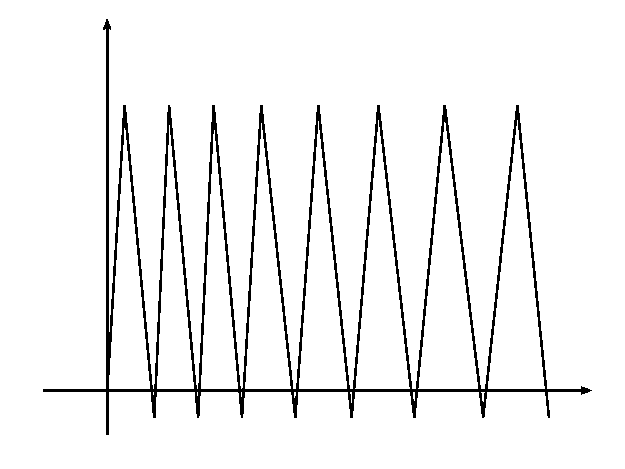
\includegraphics{img/adaptive_quadrature.pdf}
    \caption{Motivational example for adaptive quadrature}
    \label{img:adaptive-quadrature}
  \end{center}
\end{figure}

Use a problem-adjusted grid with \emph{adaptive step size} $\delta_j = t_{j+1} \cdot t_j$ with respect to the desired tolerance.

\emph{Idea}: use an \emph{adaptive quadrature} which is based on the a-posteriori estimate of the integration error
\[ \varepsilon_a^b(f) \coloneqq \hat{I}_a^b(f) - I_a^b(f) \]
Processes of adaptive quadrature are successive applications of a cycle consisting of steps.

\[
  \underbrace{\text{solution}}_{\hat{I}_a^b(f)}
    \implies \underbrace{\text{estimate}}_{\substack{\text{error estimate} \\ \text{by a quadrature} \\ \text{formula of higher order}}}
    \implies \text{marking}
    \implies \underbrace{\text{refinement}}_{\text{bijection}}
\]

\dateref{2018/12/11}

\begin{description}
  \item[Solution] Computation of approximation value $\hat{I}^{(l)}(f)$, $l \in \mathbb N_0$ using a quadratur formula, eg, trapezoidal rule with respect to some given decomposition,
    \[ \triangle_l \coloneqq \Set{a = t_0^{(l)} < t_1^{(l)} < \dots < t_{n_l}^{(l)} = b} \]
    of the integration domain $[a, b]$ in its subintervals $\triangle_{l, i} \coloneqq [t_i^{(l)}, t_{i+1}^{(l)}]$ of length $\Abs{\triangle_{l, i}} = t_{i+1}^{(l)} - t_i^{(l)}$ with $0 \leq i \leq n_l - 1$. In the following we consider the quadrature formula as \emph{basis procedure} and $l$ as the step of the refinement process.
  \item[estimate] consists of estimate of the integration error
    \[ \varepsilon^{(l)}(f) \coloneqq \hat{I}^{(l)}(f) - I(f) \]
    based on a posteriori data (with desirably little computational requirements).
  \item[marking] marks---based on the error estimate---the intervals $\triangle_{l,i}$, that should be refined for some more precise approximation. For $l \geq 1$ and $i \in \Set{0, \dots, m_l-1}$, we call $\triangle_{l,i}$ some interval of step $s(\triangle_{l,i}) = l$, if $\triangle_{l,i}$ is created by bisection of some interval from $\triangle_{l-1}^M$. Otherwise $\triangle_{l,i}$ corresponds to some interval of decomposition $\triangle_{l-1}$ and therefore $s(\triangle_{l,i}) \geq l-1$. We denote the set of intervals marked for refinement with $\triangle_l^M$.
  \item[refinement] uses some bisection of $\triangle_{l,i} = \begin{bmatrix} t_i^{(l)} & \dots & t_{i+1}^{(l)} \end{bmatrix}$ in two subintervals
    \[
      \triangle_{l,i} \coloneqq \begin{bmatrix} t_i^{(l)} & \frac{t_i^{(l)} + t_{i+1}^{(l)}}{2} \end{bmatrix}
      \triangle_{l,i}^+ \coloneqq \begin{bmatrix} \frac{t_{i+1}^{(l)} + t_{i}^{(l)}}{2} & t_{i+1}^{(l)} \end{bmatrix}
    \]
\end{description}
For the estimate of the integration error $\varepsilon^{(l)}(f)$ look for some simple-to-compute and localizable estimate $\eta_l$ of form $\eta_l = \sum_{i=0}^{n_l-1} \eta_{\triangle_{l,i}}$ where $\eta_{\triangle_{l,i}}$ with $0 \leq i \leq n_l-1$ represents estimates of integration errors $\varepsilon_{\triangle_{l,i}}(f)$ with respect to subintervals $\triangle_{l,i}$. We call estimator $\eta_l$ \emph{reliable}, if the constant $\Gamma > 0$ exists, such that $\Abs{\varepsilon^{(l)}(f)} \leq \Gamma_{\eta_l}$. We call it \emph{efficient} if $\gamma \eta_l \leq \Abs{\varepsilon^{(l)}(f)}$ with some constant $\gamma > 0$.

For some given tolerance we want to abort the adaptive refinement process, if $\eta_{l} \leq$ tolerance. Reliable estimators also guarantee a uniform magnitude for the integration error. Efficient estimators ensure that integration errors are not overestimated too much. In the perfect case, we have $\gamma_l \Gamma \approx 1$.

\emph{Idea:} Construct an estimator by using two quadrature formulas of different order, eg. Simpson's rule $\hat{I}(f)$ for basis processes.
\begin{center}
  trapezoidal rule $\equiv \hat{I}(f)$
\end{center}

Therefore we assume that
\[ \Abs{\tilde\varepsilon_{\triangle_{l,i}}^{(l)}(f)} \leq q \Abs{\varepsilon_{\triangle_{l,i}}^{(l)}(f)} \qquad 0 \leq q < 1 \]
Correspondingly we define
\[ \eta_{\triangle_{l,i}} \coloneqq \Abs{\hat{I}_{\triangle_{l,i}}^{(l)}(f) - \tilde I_{\triangle_{l,i}}^{(l)}(f)} \]
as estimator of the local integration error $\varepsilon_{\triangle_{l,i}}^{(l)}(f)$. By the triangle inequality, we get
\begin{align*}
  \Abs{\varepsilon_{\triangle_{l,i}}^{(l)}}
    &= \Abs{\hat I_{\triangle_{l,i}}^{(l)}(f) - I(f)} \\
    &= \Abs{\hat I_{\triangle_{l,i}}^{(l)}(f) - \tilde I_{\triangle_{l,i}}^{(l)}(f)} + \Abs{\tilde I_{\triangle_{l,i}}^{(l)}(f) - I(f)} \\
    &\leq \eta_{\triangle_{l,i}} + \Abs{\tilde \varepsilon_{\triangle_{l,i}}^{(l)}(f)} \\
    &\leq \eta_{\triangle_{l,i}} + q \Abs{\varepsilon_{\triangle_{l,i}}^{(l)}(f)}
\end{align*}
At the same time we have,
\[ \Abs{\varepsilon_{\triangle_{l,i}}^{(l)}(f)} \geq \eta_{\triangle_{l,i}} - \Abs{\tilde\varepsilon_{\triangle_{l,i}}^{(l)}(f)} \]
Therefore $\eta_{\varepsilon_{l,i}}$ is a reliable ($\Gamma = \frac1{1-q}$) and efficient ($\gamma = \frac1{1 + q}$) estimator at some subinterval $\triangle_{l,i}$. For marking in the adaptive cycle we assume that the local estimators $\eta_{\triangle_{l,i}}$ with constants $\kappa > 1$ and $c > 0$ behave like $\eta_{\triangle_{l,i}} \dot{=} c\Abs{\triangle_{l,i}}^\kappa$. We denote $\triangle_{l-1,j_i}$ and $j_i \in \Set{0, \dots, n_l-1}$ the interval at step $\leq l-1$ which contains $\triangle_{l,i}$. If $\triangle_{l-1,j_i} \in \triangle_{l-1}^M$, we have $\Abs{\triangle_{l-1,j_i}} = 2 \Abs{\triangle_{l,i}}$ and it follows that 
\[ \eta_{\triangle_{l-1,j_i}} \dot{=} 2^\kappa \eta_{\triangle_{l,i}} \]
Recognize that
\[ 2^{-\kappa} \dot{=} \frac{\eta_{\triangle_{l,i}}}{\eta_{\triangle_{l-1,j_i}}} \]
Because $\Abs{\triangle_{l,i}}^{I} = \frac{\triangle{l,i}}{2}$, we get
\[ \eta_{\triangle_{l,i}^{\pm}} \dot{=} C 2^{-\kappa} \Abs{\triangle_{l,i}}^\kappa \dot{=} \frac{\eta_{\triangle_{l,i}}^2}{\eta_{\triangle_{l-1,j_i}}} \eqqcolon \overline{\eta}_{\triangle_{l,i}} \]

To process step marking, we use the maximum $m_{\eta_l} \coloneqq \max_{s(\triangle_{l,i})=l} \overline{\eta_{\triangle_{l,i}}}$ of local estimators $\eta_{\triangle_{l,i}}$ with $s(\triangle_{l,i}) = l$. For some given $\theta \in (0,1)$ we mark all subintervals $\triangle_{l,i}$ for refinement for which $\eta_{\triangle_{l,i}} \geq \theta m_{\eta_l}$. As termination condition we compare $\hat I^{(l)}_{[a,b]}(f)$ with $\hat I_{[a,b]}^{(l-1)}(f)$.
\[ \varepsilon_{\text{rel}}^{(l)} \coloneqq \frac{\Abs{\hat I_{[a,b]}^{(l)}(f) - \hat I_{[a,b]}^{(l-1)}(f)}}{\Abs{\hat I_{[a,b]}^{(l)}(f)}} \leq \text{ tolerance} \]

\begin{algorithm}
  \begin{enumerate}
    \item Input: $f, \triangle_0, \theta \in (0,1]$ and tolerance $> 0$
    \item for $l = 0, 1, \dots$
      \begin{enumerate}
        \item Determine $\hat I_{l,i}^{(l)}(f), \hat{I}_{\triangle_{l,i}}^{(l)}(f), \eta_{\triangle_{l,i}}$ and $\hat{I}_{[a,b]}^{(l)}(f)$
        \item if $l = 1$
          \begin{enumerate}
            \item Determine $\varepsilon_{\text{rel}}^{(l)}$
            \item if $\varepsilon_{\text{rel}}^{(l)} \leq$ tolerance
              \begin{enumerate}
                \item Terminate with solution $I_{[a,b]}^{(l)}(f)$
              \end{enumerate}
          \end{enumerate}
        \item for $i = 0, 1, \dots, m_l - 1$
          \begin{enumerate}
            \item Determine $\hat{\eta_{\triangle_{l,i}}}$ for $\triangle_{l,i}$
          \end{enumerate}
        \item Compute $m_{\eta_{l}}$
        \item Create $\triangle_{l+1}$ by bisection of all $\triangle_{l,i}$ for which $\eta_{\triangle_{l,i}} \geq \theta_{\eta_l}$
      \end{enumerate}
  \end{enumerate}
\end{algorithm}

\subsection{Multidimensional quadrature}

\emph{Goal:} Overview how to generalize quadrature formulas over domains $D \subset \mathbb R^n$. \\
\emph{Idea:} Reduce to integration of standard domains

\paragraph{Transformation of integrals}

Reduce from $\int_a^b$ to $\int_c^d$ by expressing a coordinate transformation by some bijective, continously differentiable map $\Psi: [c, d] \to [a, b]$. Variable transformation $x = \Psi(t)$ gives 
\[ \int_a^b f(x) \, dx = \int_c^d f(\Psi(t)) \Psi'(t) \, dt \]
For the special case of affine maps $\Psi(t) = \alpha t + \beta$ with $\alpha, \beta \in \mathbb R$, the parameters are distinctly given by $\Psi(c) = a$ and $\Psi(d) = b$.

Thus, intervals are mapped the intervals for $\alpha \neq 0$. Furthermore it holds that $p(x)$ is a polynomial of degree $n$ in $x$, then $p(\Psi(t))$ a polynomial of degree $n$ in $t$.

The accuracy of the quadrature formula is not affected.

In $\mathbb R^n$, we use an analogous approach. We integrate over some domain $B_1$ using some quadrature formula for $B_2$. Affine maps have the form
\[  \Psi: B_2 \to B_1 \qquad \Psi(t) = At + c: A \in \mathbb R^{n \times n}, c \in \mathbb R^{n} \]
and are uniquely defined by predefining the transformation of $n+1$ points ($n(n+1)$ equations for $n^2 + n$ parameters in $A$ and $c$). The transformation formula is then given by
\[ \int_{B_1} f(x) \, dx = \int_{B_2} f(\Psi(t)) \cdot \Abs{\det(\nabla \Psi(t))} \, dt \]
where $\nabla \Psi(t)$ denotes the Jacobian matrix of $\Psi$. In the affine case, we have $\nabla \Psi(t) = A$

\paragraph{Integration over standard square}

We consider $f: Q \to \mathbb R$ and $Q = [0, 1] \times [0, 1] \subset \mathbb R^2$
\[ \iint_{Q} f(x, y) d(x, y) = \int_0^1 \int_0^1 f(x, y) \, dx \, dy \]
The integration boundaries for $x$ depend not on $y$ and we can insert separate quadrature formulas for $x$ and $y$.
\begin{align*}
  \int_0^1 \int_0^1 f(x, y) \, dx \, dy
    &= \int_0^1 F(y) \, dy \\
    &\approx \sum_{j=0}^n \lambda_j F(y_j) \\
    &= \sum_{j=0}^n \lambda_j \int_0^1 f(x, y_j) \, dx \\
    &\approx \sum_{j=0}^n \lambda_j \sum_{k=0}^n \lambda_k f(x_k, y_j) \\
    &= \sum_{j,k=0}^n \lambda_j \lambda_k \cdot f(x_k, y_j)
\end{align*}
with points and weights $(y_j^\kappa, \lambda_j)$, and accordingly $(x_\kappa, \lambda_\kappa)$.

If the quadrature formulas are exactly of degree $m$, then functions of form $x^k y^j$, $0 \leq k, j \leq m$ are integrated accurately. The approximation error can be derived by the error representation of one-dimensional quadrature formulas.

\dateref{2018/12/13}

\paragraph{Integration over default triangle}

We consider $f: T \to \mathbb R, T = \SetDef{(x,y)}{0 \leq x \leq 1, 0 \leq y \leq 1 - x} \subset \mathbb R^2$.
\[ \iint_T f(x, y) \, d(x,y) = \int_0^1 \int_0^{1\cdot x} f(x, y) \, dy \, dx \]
Here, integration boundaries are not independent in $x$ and $y$ (and therefore the supporting points).
Thus consider the quadrature formulas of form
\[ \sum_{j=0}^n \lambda_j f(x_j, y_j) \approx \iint_T f(x, y) d(x, y)  \]
We require that polynomials of form $x^k y^j$, $0 \leq k + j \leq m$, are integrated accurately. for $m \geq 2$ e.g. the polynomials $1, x, y, x^2, xy, y^2$ (those create an orthogonalbasis wrt. scalar product $\IP{f}{g} = \iint_T f(x, y) g(x, y) \, d(x, y)$).

So, in $\mathbb R^n$ there exists for all $m$ some quadrature formula of accuracy $m$, that requires only ${m+n \choose n}$ supporting points.

These are not unique.

\begin{table}[t]
  \begin{center}
    \begin{tabular}{ccc}
      $(x_j, x_j)$ & $\lambda_j$ & accurately \\
    \hline
      $(\frac 13, \frac 13)$ & $\frac12$ & 1 \\
      $(0, 0), (1, 0), (0, 1)$ & $\frac 16$ & 1 \\
      $(\frac12, \frac12), (\frac12, 0), (0, \frac12)$ & $\frac16$ & 2 \\
      $(\frac16, \frac16), (\frac23, \frac16), (\frac16, \frac23)$ & $\frac16$ & 2
    \end{tabular}
    \caption{The first line corresponds to the Gauss quadrature on $T$}
  \end{center}
\end{table}

\subsection{Higher dimensional integrals}

\emph{Question:} How do we compute higher dimensional integrals $\int_Q f(x) \, dx$ for, for example, $Q = \prod_{i=1}^{d} [a_i, b_i]$.
\[ \text{Fubini's Theorem } \implies \int_Q f(x) \, dx = \int_{a_d}^{b_d} \dots \int_{a_1}^{b_1} f(x_1, \dots, x_d) \, dx_1 \dots dx_d \]
Use one-dimensional quadrature formulas:
Consider e.g. $Q = [0, 1]^d$ and $f$ arbitrary. For $d=1$ we get by trapeziodal sum the approximation
\[ \int_0^1 f(x) \, dx \approx \sum_{i=0}^n \lambda_i f\left(\frac in\right) \]
with $\lambda_0 = \lambda_n = \frac1{2n}$ and $\lambda_i = \underbrace{\frac1m}_{k}$ for $i \neq 0, n$.

In the multidimensional case we analogously get
\[ \int_a f(x) \, dx = \int_0^1 \dots \int_0^1 f(x_1, \dots, x_d) \, dx_1 \dots dx_d \approx \sum_{j_1=0}^n \dots \sum_{j_d=0}^n \lambda_{j_1} \dots \lambda_{j_d} f\left(\frac{j_1}{m}, \dots, \frac{j_d}{m}\right) \]
The number of evaluations is $N = (n+1)^d$. For $d = 1$ and $f \in \mathcal C^2([0, 1])$ we know that the integration error behaves like $\mathcal O(\frac1{n^2})$. For $d \geq 2$, this value does not improve (consider the special case $f(x_1, \dots, x_d) = g(x_1)$). The approximation error of the quadrature formula above behaves like $\mathcal O(\frac 1{n^2}) = \mathcal{N^{-\frac 2d}}$.

For large $d$ the error margin decreases. To halve the approximation error, we need to apply $2^{\frac d2}$ more function evaluations (\emph{curse of dimensionality}).

\begin{Remark}
  The following paragraph is not relevant for exams.
\end{Remark}

\paragraph{Monte-Carlo integration}

In the following, we denote the Lebesgue measure on $\mathbb R^d$ with $\gamma$.
For $Q \coloneqq \prod_{i=1}^d [a_i, b_i]$ we have $\gamma(Q) = \prod_{i=1}^{d} (b_i - a_i)$.
For some integration domain $B$ with $0 < \gamma(B) < \infty$, we consider the probability space ($B, d(B), \mu$) with Lebesgue-measurable subsets of $B$ and the probability measure $\mu = \frac{\gamma}{\gamma(B)}$. For some function $f \in \mathcal C(B)$ we have
\[ \int_B f \, d\gamma(x) = \gamma(B) \cdot \int_B f(x) \, d\mu(x) = \gamma(B) \cdot \mathcal E(f(X)) \]
where $X$ is a uniform random variable distributed among $B$.

\dateref{2018/01/08}

\section{Non-linear equation systems}

\subsection{Theoretical preliminaries}

\emph{Problem setting:} Let $f: \mathbb R^n \to \mathbb R^n$ continuous. Find its roots $s$ such that $f(s) = 0$.

We consider a system of $n$ unknown variables:
\[ f_1(s_1, \dots, s_n) = 0 \qquad f_n(s_1, \dots, s_n) = 0 \]

\emph{Idea:} Formulate the system as (equivalent) fixed point problem of form $f(s) = 0 \iff s = F(s) \implies$ s is a fixed point of $F$.

\index{Fixed point iteration}
\index{Single-level, stationary iteration process}
This immediately gives an iteration process to solve the equation system:
$x^{(k + 1)} = F(x^{(k)}), k \in \mathbb N_0$ with $x^{(k)} \in \mathbb R^n$.
This iterative equation is called \emph{Fixed point iteration}.
Because for computation of $x^{(k+1)}$ only $x^{(k)}$ is required,
this process is also called \emph{single-level, stationary iteration process}\footnote{stationary here means independence of $k$}.

\begin{example}
  \label{ex:6-1}
  \[ f\begin{pmatrix} x_1 \\ x_2 \end{pmatrix} = \begin{pmatrix} x_1^2 + x_2 - 4 \\ x_2 e^{x_1} - 2 \end{pmatrix} \]
  \[
    \implies \begin{array}{cc}
      f_1(x) &= x_1^2 + x_2 - 4 \\
      f_2(x) &= x_2 e^{x_1} - 2
    \end{array}
  \]
  Resolve by $x_2$:
  \begin{align*}
    x_2 &= 4 - x_1^2 \eqqcolon g_1(x_1) \\
    x_2 &= 2 \cdot e^{-x_1} \eqqcolon g_2(x_1) \\
  \end{align*}
  Visualized in Figure~\ref{img:intersection}.
  
  \begin{figure}[!ht]
    \begin{center}
      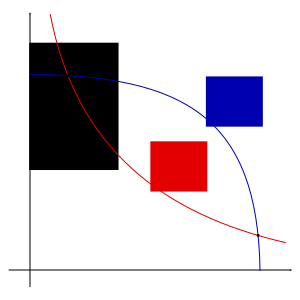
\includegraphics{img/intersection.pdf}
      \caption{We look for intersection points of $g_1$ and $g_2$}
      \label{img:intersection}
    \end{center}
  \end{figure}

  We retrieve a fixed point equation, for example, by resolving the first equation by $x_1$, the second by $x_2$, \dots.
  \[ F_1(x_1, x_2) \coloneqq \sqrt{4 - x_2} \qquad F_2(x_1, x_2) \coloneqq 2 \cdot e^{-x_1} \]
  Resolving it the other way around is, of course, also okay.
  \[ x_1 = \ln(\frac2{x_2}) \eqqcolon \tilde F_1(x_1, x_2) \]
  \[ x_2 = 4 - x_1^2 \eqqcolon \tilde F_2(x_1, x_2) \]

  \begin{figure}[!ht]
    \begin{center}
      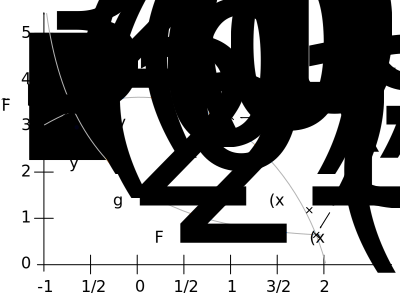
\includegraphics{img/fixed_point_iteration.pdf}
      \caption{Fixed point iteration}
      \label{fig:fpi}
    \end{center}
  \end{figure}

  Compare with Figure~\ref{fig:fpi}.
  Our conclusion is: even though we have the same initial value, $F$ and $\tilde F$ converge towards different solutions.
  Thus, convergence and uniqueness is not given in general.
\end{example}

\paragraph{Convergence theory}

\begin{definition}[Convergence]
  \label{definition:6-2}
  The sequence $(x^{(k)})_{k \in \mathbb N_0}$ has \emph{convergence order} of at least $p \geq 1$ if $\exists K > 0$ (where $K$ is independent of $k$):
  $\Norm{x^{(k+1)} - s} \leq K \cdot \Norm{x^{(k)} - s}^p \forall k \geq 0, K < 1 \text{ if } p = 1$

  Then $K$ is called \emph{convergence rate} or \emph{error rate}.
\end{definition}

\begin{Remark}
  The convergence rate is called linear/quadratic/cubic if $p = 1$, $2$ or $3$ respectively.

  (In practice it is $p \leq 3$)
\end{Remark}

\index{Lipschitz-continuity}
\index{Contraction}
\begin{definition}
  For a closed subset $A \subseteq B$ and Banach space $B$,
  let $f: A \to A$ be a map.
  $f$ is called \emph{Lipschitz-continuous} on $A$ with constant $0 < L < \infty$
  if \[ \Norm{f(y) - f(x)} \leq \Norm{x - y} \cdot L \qquad \forall x, y \in A \]
  $f$ is called \emph{contraction} (or \emph{contracting}) on $A$ if $L < 1$.
\end{definition}

\begin{theorem}[Banach Fixed Point]
  \label{theorem:6-4}
  Let $A \subseteq B$ be a non-empty, closed subset of a Banach space $B$.
  $F: A \to A$ is a contraction. Then:
  \begin{enumerate}
    \item $F$ has exactly one fixed point $s \in A$
    \item For every $x^{(0)} \in A$ with $x^{(k)} \coloneqq F(x^{(k-1)})$, $(x^{(k)})$ converges to $s$.
    \item $\Norm{x^{(k)} - s} \leq L^k \cdot \Norm{x^{(0)} - s}$
    \item A-priori error estimate: $\Norm{x^{(k)} - s} \leq \Norm{x^{(1)} - x^{(0)}} \cdot \frac{L^k}{1 - L}$
    \item A-posteriori error estimate: $\Norm{x^{(k)} - s} \leq \frac{L}{1 - L} \cdot \Norm{x^{(k)} - x^{(k - 1)}}$
  \end{enumerate}
\end{theorem}

\begin{proof}
  For the difference of two consecutive iterands, we get:
  \begin{align*}
    \Norm{x^{(k+1)} - x^{(k)}} &= \Norm{F(x^{(k)}) - F(x^{(k-1)})} \cdot L \\
      &\leq L \cdot \Norm{x^{(k)} - x^{(k-1)}} \\
      &= \dots \\
      &\leq L^{k - l} \cdot \Norm{x^{(l+1)} - x^{(l)}} \quad \text{ for } 0 \leq l \leq k
  \end{align*}
  \[ f: A \to A \qquad \text{ thus } x^{(0)} \in A \implies x^{(k)} \in A \forall k \]
  By this we conclude that $\Set{x^{(k)}}$ is a Cauchy sequence:
  \begin{align*}
    \Norm{x^{(k+m)} - x^{(k)}}
      &= \Norm{x^{(k+m)} - x^{(k+m-1)} + x^{(k+m-1)} \dots + x^{(k)}} \\
      &\leq \sum_{u = k}^{k + m - 1} \Norm{x^{(u+1)} - x^{(u)}} \\
      &\leq L^k \cdot (L^{m-1} + L^{m-2} + \dots + L + 1) \\
      &= L^k \cdot \frac{1 - L^m}{L} \cdot \Norm{x^{(1)} - x^{(0)}}
  \end{align*}
  Because $L < 1$, the last equation is a zero sequence. Hence $\Set{x^{(k)}}$ is a Cauchy sequence.

  $A$ is complete, so $\exists s: s = \lim x^{(k)}, s \in A$.

  By continuity of $F$, we have
  \[ F(s) = F(\lim{x^{(k)}}) = \lim F(x^{(k)}) = \lim x^{(k+1)} = s \]
  Hence, $\Set{x^{(k)}}$ converges to a fixed point.

  Uniqueness: Let $s_1$ and $s_2$ be fixed points of $F$.
  \[ \implies \Norm{s_1 - s_2} = \Norm{F(s_1) - F(s_2)} \leq L \cdot \Norm{s_1 - s_2} \]
  \[ L < 1 \implies \Norm{s_1 - s_2} = 0 \]

  For fixed $k$ and $m$, $\Norm{x^{(k+m)} - x^{(k)}} \leq L^k \cdot \frac{1 - L^m}{L} \cdot \Norm{x^{(1)} - x^{(0)}}$ gives the a-priori error estimate.

  The third claim results from
  \[ \Norm{x^{(k)} - s} = \Norm{F(x^{(k-1)}) - s} \leq L \cdot \Norm{x^{(k-1)} - s} \leq \dots \leq L^k \cdot \Norm{x^{(0)} - s} \]
  The a-posteriori error estimate follows by the a-priori error estimate by rearrangement of $x^{(k-1)}$ as $\tilde x^{(0)}$.
\end{proof}

\begin{Remark}
  Determination of $A$ is difficult for practical problems.
\end{Remark}

\begin{theorem}
  \label{theorem:6-5}
  Let $n=1$. In the closed neighborhood $A$ of fixed point $s$, let the iteration function $F$ satisfy $F \in \mathcal C^1(A)$.
  Then the process is at least linear convergent, if $\Abs{F'(s)} < 1$.

  The process is of $p$-th order if $F^{(k)}(s) = 0$ for $k \in \Set{1, \dots, p-1}$.
\end{theorem}

\begin{proof}
  The proof will be given in the practicals.
\end{proof}

\paragraph{Condition, Stability}

Cases (compare with Figure~\ref{fig:three-cases}):
\begin{enumerate}
  \item $f$ has only complex roots and some algorithm capable of handling complex numbers must be used.
  \item $f$ has only once root with multiplicity 2. This is considered ill-conditioned, because an arbitrary small deviation can lead to two or zero roots.
  \item We have two well-distinguishable roots. This is considered a stable situation.
\end{enumerate}

\begin{figure}[!ht]
  \begin{center}
    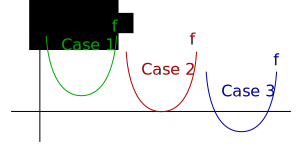
\includegraphics{img/three_cases.pdf}
    \caption{Three cases for roots of $f$}
    \label{fig:three-cases}
  \end{center}
\end{figure}

If we consider some interval $[x_-, x^+]$ around each root such that $\Abs{f(x)} < \varepsilon \forall x \in [x_-, x_+]$.
This gives either case 3 or case 2 (if only one).

\subsection{Equation in one unknown}
\label{ch:6-2}

In the following, we consider the task for continuous, non-linear functions $f: \mathbb R \to \mathbb R$ restricted to real solutions.

\begin{algorithm}
  \emph{Idea:} We decrease the intervals to consecutively approximate the real solution.

  \emph{Assumption:} $I = [a, b]$, $f(a) \cdot f(b) < 0$. Because $f$ is continuous there exist roots in $I$.

  \begin{itemize}
    \item Compute the function value $f(\mu)$ with $\mu \coloneqq \frac{a + b}{2}$. If $\operatorname{sign}(f_\mu) = \sign{f(a)}$, we get a new interval $I = [\mu, b]$. $\sign{f(\mu)} = \sign{f(b)} \implies I = [a, \mu]$. $\sign{f(\mu)} = 0$ gives the result.
    \item Nested intervals: $\Abs{I^{(n)}} = \frac{b - a}{2^n} = $ zero sequence.
    \item We can find a unique $s$.
      The midpoint $x^{(k)}$ of $I^{(k)}$ satisfies the a-priori estimate $\Abs{x^{(k)} - s} \leq \frac{b - a}{2^{k+1}}$.
    \item This corresponds to an average linear convergence ($p = 1$).
  \end{itemize}
\end{algorithm}

\paragraph{Newton method}

\emph{Idea:} Consider the linear function through $x^{(0)}$. Choose $x^{(1)} \coloneqq$ roots.

\dateref{2018/01/10}

\paragraph{Newton's method}

Let $f \in \mathcal C^1, f^1(x^{(k)})$ computable. Then we create $x^{(k+1)}$ as root of linearization of $f$ in $x^{(k)}$. By the tangent equation
\[ t(x) = f(x^{(k)}) + (x - x^{(k)})f'(x^{(k)}) \]
and the requirement $t(x^{(k+1)}) = 0$ we retrieve the iteration rule:
\[ x^{(k+1)} = x^{(k)} - \frac{f(x^{(k)})}{f'^(x^{(k)})} \qquad k = 0, 1, 2, \dots \]
The Newton's method is part of the class of fixed point iterations with the function
\[ F(x) \coloneqq x - \frac{f(x)}{f'(x)} \]
and for the fixed point $s = F(s)$ we have $f(s) = 0$.

\begin{theorem}
  \label{theorem:6-2}
  Let $f \in \mathcal C^2([a, b])$ with $a < s < b$ and $f'(s) \neq 0$, hence, $s$ is a simple root of $f$.
  Then there exists some interval $I = [s - \delta, s + \delta]$, $\delta > 0$ for which $F: I \to I$, $F(x) = x - \frac{f(x)}{f'(x)}$ is a contracting map. For every initial value $x^{(0)} \in I$, the sequence of the Newton's method is at least quadratically convergent.
\end{theorem}

\begin{proof}
  We show that $\Abs{F'(x)} < 1$ in some neighborhood $U_\delta(s)$. For $F'$ we get
  \[ F'(x) = 1 - \frac{f'(x)^2 - f(x) \cdot f''(x)}{f'(x)^2} = \frac{f(x) f''(x)}{f'(x)^2} \]
  and thus $F'(s) = 0$ by $f(s) = 0$. Because $F'$ is continuous, there exists some $\delta > 0$,
  such that $-1 < F'(s) < 1$ for all $x \in [s - \delta, s + \delta] = I$.

  By Theorem~\ref{theorem:6-5} and the Banach's Fixed Point Theorem, the convergence of sequence $\Abs{x^{(k)}}$ to $s$ and the convergence order is at least $p = 2$.
\end{proof}

\begin{example}[for divergence]
  Consider $f(x) = x^3 - 2x + 2$ with $x^{(0)} = 0$ and $f'(x) = 3x^2 - 2$.
  \[ x^{(1)} = x^{(0)} - \frac{f(x^{(0)})}{f'(x^{(0)})} = 1 \]
  \[ x^{(2)} = x^{(1)} - \frac{f(x^{(1)})}{f'(x^{(1)})} = 1 - \frac11 = 0 \]
  The Newton's method obviously does not converge.
  Furthermore we can shown that neighborhoods at 0 and 1 exist, that attract this cycle.

  TODO drawing

  Be aware that convergence is given only locally!
\end{example}

\begin{example}
  \label{example:6-8}
  The n-th root of a positive number $a$ is the solution of $f(x) = x^m - a$ with $a > 0$.
  The Newton method with $f'(x) = mx^{m-1}$ the rule
  \[ x^{(k+1)} = x^{(k)} - \frac{(x^{(k)})^m - a}{m(x^{(k)})^{m-1}} = \frac{a + (m - 1) (x^{(k)})^m}{m (x^{(k)})^{(m-1)}} \]
  And accordingly,
  \[ x^{(k + 1)} = \frac1m \left(\frac{a}{(x^{(k)})^{m-1}} + (m-1) x^{(k)}\right) \qquad k = 0, 1, 2, \dots \]
  Thus we get the special cases,
  \[ x^{(k+1)} = \frac12 \left(\frac{a}{x^{(k)}} + x^{(k)}\right) \qquad \text{\enquote{square root}} \]
  \[ x^{(k+1)} = \frac13 \left(\frac{a}{(x^{(k)})^2} + 2x^{(k)}\right) \qquad \text{\enquote{cubic root}} \]
  \[ x^{(k+1)} = (2 - ax^{(k)}) x^{(k)} \qquad \text{\enquote{reciprocal}} \]
\end{example}

\dateref{2019/01/15}

\paragraph{Two variants of the Newton method}

\index{Stabilized Newton method}

\begin{itemize}
  \item The simplified Newton method
    \[ x^{(k+1)} = x^{(k)} = \frac{f(x^{(k)})}{f'(x^{(0)})} \qquad k = 0, 1, 2, \dots \]
    Because the first derivatives do not change in the last iteration steps, this process is usefuv for \enquote{good} initial values $x^{(0)}$.

    The disadvantage is that the convergence order is only $p = 1$,
    but often with small error constant $k$.
  \item The \emph{stabilized} Newton method
    \[ x^{(k+1)} = x^{(k)} - \lambda_k \frac{f(x^{(k)})}{f'(x^{(k)})} \qquad k = 0, 1, 2, \dots \]
    avoids convergence issues by division by 2 of $\lambda_k$ until $\Abs{f(x^{(k+1)})} < \Abs{f(x^{(k)})}$.
\end{itemize}

\paragraph{Secant method}

\emph{Idea:}
  Avoid computation of the derivative and use the secant:
  we need two initial values $x^{(0)} \neq x^{(1)}$
  (no restriction on $x^{(0)}$ and $x^{(1)}$ as in the bisection process)

We get the following iteration step:
\[ x^{(k+1)} = x^{(k)} - f(x^{(k)}) \frac{x^{(k)} - x^{(k-1)}}{f(x^{(k)}) - f(x^{(k-1)})} \]
The secant method is a two-level iteration process.
For well-definiteness of the iteration we require $f(x^{(k)}) \neq f(x^{(k-1)})$.

\begin{theorem}
  \label{theorem:6-9}
  If $f'(s) \neq 0$ and $f''(s) \neq 0$,
  the convergence order of the secant method is $p = \frac 12 (1 + \sqrt{5}) \dot= 1.618$.
\end{theorem}

\begin{proof}
  Refer to the book by Schwarz
\end{proof}

\subsection{The Newton method in $\mathbb R^n$}

Again, we consider systems of non-linear equations $f(x) = 0$,
where $f: \mathbb R^n \to \mathbb R^n$ is a continuously differentiable function with specific, additional properties.
Like before, we substitute the function $f$ locally by an affine-linear function.
The Taylor expansion of $f$ at some initial value $x^{(0)}$ gives
\[ 0 = f(x) = \underbrace{f(x^{(0)}) + f'(x^{(0)}) (x - x^{(0)})}_{\eqqcolon \overline{f}(x)} + \mathcal o(\Norm{x - x^{(0)}}) \text{ for } x \to x_0 \]

Thus, the root $x^{(1)}$ of the map $\overline f$ is
\[ x^{(1)} = x^{(0)} - f'(x^{(0)})^{-1} f(x^{0}) \]
assuming that the Jacobian matrix $f'(x^{(0)})$ is invertible at $x^{(0)}$.
This leads to the following Newton iteration:
\[ f'(x^{(k)}) \triangle x^{(k)} = -f(x^{(k)}) \]

\index{Newton correction}
Recognize: Avoid explicit computation of inverse $f'(x^{(k)})^{-1}$ and instead solve the linear equation system for the so-called \emph{Newton correction} $\triangle x^{(k)}$.

\emph{Observation:} numeric solution of a non-linear equation system corresponds to numerical solution of a sequence of a linear equation system.

\index{Convex set}
\begin{definition}
  \label{definition:6-10}
  A set $M \subset \mathbb R^n$ is called \emph{convex} if for $x, y \in M$ it is true that $z = \lambda x + (1 - \lambda) y \in M$ for all $\lambda \in [0, 1]$.
\end{definition}

\paragraph{Convergence of the Newton method}

\begin{theorem}[Newton-Kantorovic]
  \label{theorem:6-11}
    Let $D \subset \mathbb R^n$ be an open and convex set. Furthermore let $f: D \subset \mathbb R^n \to \mathbb R^n$ continuously differentiable.
    \begin{itemize}
      \item Let the Jacobian matrix be uniformly Lipschitz-continuous for all $x, y \in D$.
        \[ \Norm{f'(x) - f'(y)} \leq \gamma \Norm{x - y} \qquad x, y \in D \]
      \item Furthermore the Jacobian matrix on $D$ has a uniform bounded inverse
        \[ \Norm{f'(x)^{-1}} \leq \beta \qquad x \in D \]
      \item For initial value $x^{(0)} \in D$, let:
        \[ q \coloneqq \alpha \beta \gamma < \frac 12, \alpha \coloneqq \Norm{f'(x^{(0)})^{-1} f(x^{(0)})} \]
      \item For $r = 2\alpha$ let the bounded sphere
        \[ B_r(x^{(0)}) \coloneqq \SetDef{x \in \mathbb R^n}{\Norm{x - x^{(0)}} \leq r} \]
        be contained in $D$.
    \end{itemize}
  Then the function $f$ has a root $z \in B_r(x^{(0)})$ and the Newton iteration
  \[ f'(x^{(k)}) \triangle x^{(k)} = -f(x^{(k)}) \qquad x^{(k+1)} = x^{(k)} + \triangle x^{(k)} \qquad k = 0, 1, 2, \dots \]
  converges quadratically towards root $z$.
  Furthermore the following a-priori error estimate is true,
  \[ \Norm{x^{(k)} - z} \leq 2\alpha q^{2^k - 1} \qquad k = 0, 1, 2, \dots \]
\end{theorem}

\begin{proof}
  The proof consists of the following steps:
  \begin{enumerate}
    \item Deduction of an auxiliary estimate
    \item All iterands are in $B_r(x_{(0)})$
      and some a-priori error estimate for $\Norm{x^{(k)} - x^{(0)}}$ is true (\dots induction)
    \item Show $\Set{x^{(k)}}$ is a Cauchy sequence and thus has a unique limit $z$ in $\mathbb R^n$
    \item Show existence of a root, $z$ is a root
    \item Uniqueness of a root $z$
  \end{enumerate}

  So, we begin
  \begin{enumerate}
    \item Let $x, y, z \in D$. Because $D$ is convex, for all $x, y \in D$ we have
      \[ f_j(x) - f_j(y) = \int_0^1 \frac{d}{ds} f_j(sx + (1 - s) y) \, ds \qquad j = 1, \dots, n \]
      By the chain rule, we get
      \[ \frac{d}{ds} f_j(sx + (1 - s)y) = \sum_{k=1}^n \frac{\partial f_j}{\partial x_k} (sx + (1 - s) y) (x_k - y_k) \]
      and therefore
      \[ f_j(x) - f_j(y) = \int_0^1 \sum_{k=1}^n \frac{\partial f_j}{\partial x_k} (sx + (1 - s) y) (x_k - y_k) \, ds \]
      We can also denote it as,
      \[ f(x) - f(y) = \int_0^1 f'(sx + (1 - s)y)(x - y) \, ds \]
      By insertion of $f'(z)(x - y)$ we conclude
      \[ f(x) - f(y) - f'(z)(x - y) = \int_0^1 (f'(s x + (1 - s)y) - f'(z)) (x - y) \, ds \]
      By the Lipschitz continuity of $f'$, we get
      \[ \Norm{f(y) - f(x) - f'(z) (y - x)} \leq \gamma \Norm{y - x} \int_0^1 \Norm{s (x - z) + (1 - s) (y - z)} \, ds \]
      \[ \leq \frac \gamma2 \Norm{y - x} (\Norm{x - z} + \Norm{y - z}) \]
      For $z = x$, this gives,
      \[ \Norm{f(y) - f(x) - f'(x) (y - x)} \leq \frac{\gamma}2 \Norm{y - x}^2 \qquad \forall x, y \in D \label{eqq1} \]
      In contrast, for $z = x^{(0)}$ we get
      \[ \Norm{f(y) - f(x) - f'(x^{(0)}) (y - x)} \leq \tau \gamma \Norm{y - x} \qquad \forall x, y \in B_r(x^{(0)}) \label{eqq2} \]
    \item We use complete induction and show:
      \[ \Norm{x^{(k)} - x^{(0)}} \leq r \qquad \Norm{x^{(k)} - x^{(k-1)}} \leq \alpha q^{2^{k-1} - 1} \qquad k = 1, 2, \dots \]
      We begin with $k = 1$. By the preconditions, we have
      \[ \Norm{x^{(1)} - x^{(0)}} = \Norm{f'(x^{(0)})^{-1} f(x^{(0)})} = \alpha = \frac r2 < r \]
      Now we assume that both inequalities are true for $k \geq 1$.
      Because of the second statement and because $x^{(k)} \in B_r(x^{(0)}) \subset D$, the iterand $x^{(k+1)}$ is well-defined.
      We get
      \[ \Norm{x^{(k+1)} - x^{(k)}} = \Norm{f'(x^{(k)})^{-1}  f(x^{(k)})} \leq \beta \Norm{f(x^{(k)})} = \beta \Norm{f(x^{(k)}) - \underbrace{f(x^{(k - 1)}) - f'(x^{(k - 1)}) (x^{(k)} - x^{(k - 1)})}_{= 0}} \]
      \[ \leq \frac{\beta \gamma}{2} \Norm{x^{(k)} - x^{(k - 1)}}^2 \overset{\substack{\text{induction} \\ \text{hypothesis}}}{\leq} \frac{\beta \gamma}{2} \left(\alpha q^{2^{k - 1} - 1}\right) = \frac{\alpha}{2} q^{2^k - 1} < \alpha q^{2^k - 1} \]
      by using $q \coloneqq \alpha p \gamma$.
      This (still) implies
      \[ \Norm{x^{(k+1)} + x^{(0)}} \leq \Norm{x^{(k+1)} - x^{(k)}} + \dots + \Norm{x^{(1)} - x^{(0)}} \leq 2 (1 + q + q^3 + q^7 + \dots + q^{2^k - 1}) \leq \frac{\alpha}{1 - q} \leq 2\alpha = r \]
    \item Let $m > 0$. Because $q < \frac12$, we have
      \begin{align*}
        \Norm{x^{(k)} - x^{(k + m)}} &= \Norm{x^{(k)} - x^{(k+1)}} + \dots + \Norm{x^{(k+m-1)} - x^{(k+m)}} \\
          &\leq \alpha(q^{2^k - 1} + \dots + q^{2^{m + k - 1} - 1}) \\
          &\leq \alpha q^{2^k - 1} (1 + q^{2^k} + \dots + q^{(2^k)^{2^{m-1} - 1}}) \\
          &\leq 2 \alpha q^{2^k - 1}
      \end{align*}
      Therefore $\Set{x^{(k)}}$ is a Cauchy sequence and there exists some limes $z = \lim_{k \to \infty} x^{(k)}$. For $k \to \infty$ we have the estimate
      \[ x^{(k)} - x^{(0)} \leq r \implies \Norm{z - x^{(0)}} \leq r \]
      such that $z \in B_r(x^{(0)})$. For $m \to \infty$ we get TODO
    \item The Newton iteration and the first precondition provide:
      \begin{align*}
        \Norm{f(x^{(k)})} &= \Norm{f'(x^{(k)})(x^{(k + 1)}  - x^{(k)})} \\
          &\leq \Norm{f'(x^{(k)}) - f'(x^{(0)}) + f'(x^{(0)})} \Norm{x^{(k+1)} - x^{(k)}} \\
          &\leq \left(\gamma \Norm{x^{(k)} - x^{(0)}} + \Norm{f'(x^{(0)})}\right) \Norm{x^{(k+1)} - x^{(k)}} \to 0 \text{ if } k \to \infty
      \end{align*}
      Thus, $f(x^{(k)}) \to 0, k \to \infty$ and because of continuity of $f$ also $f(z) = 0$.
    \item The root $z$ of $f$ is also a fixed point of the simplified iteration
      \[ \overline{g}(x) = x - f'(x^{(0)})^{-1} f(x) \]
      The function $\overline{g}$ is a contraction, because
      \[ \overline{g}(x) - \overline{g}(y) = x - y - f'(x^{(0)})^{-1} (f(x) - f(y)) = f'(x^{(0)})^{-1} (f(y) - f(x) - f(x^{(0)}) (y - x)) \]
      implies the estimate
      \[ \Norm{\overline g(x) - \overline g(y)} \overset{Ineq.~\ref{eqq2}}{=} \beta \gamma r \Norm{y - x} \leq \underbrace{2q}_{= \alpha \beta \gamma} \Norm{y - x} \forall x, y \in B_1(x^{(0)}) \]
      Because $x < \frac12$, $\overline g$ is a contraction and it can have at most one fixed point.
  \end{enumerate}
\end{proof}

The main difference to the scalar case is that didn't require $f \in \mathcal C^2$.
Furthermore the existence of a root follows from the following theorem:

\begin{corollary}
  \label{corollary:6-12}
  Let $D \subset \mathbb R^n$ be open, convex and at most two times differentiable.
  Let $z \in D$ be a root with regular Jacobian matrix $f'(z)$. Then the Newton method is locally convergent, hence there exists some neighborhood $B$ at $z$ such that the Newton method converges to $z \forall x^{(0)} \in B$.
\end{corollary}

\dateref{2019/01/17}

\begin{example}[Newton method to compute the inverse]
  To determine the inverse $Z = A^{-1}$ of an invertible matrix $A \in \mathbb R^{n \times n}$ we consider:
  \[ f(x) \coloneqq X^{-1} - A \]
  for $X$ regular. First, determine a neighborhood $A$ such that $f(\cdot)$ is well-defined and differentiable.
  For this, assume $X \in B_r(A)$ with $r < \Norm{A^{-1}}^{-1}$.
  Then, by $X = A - A + X = A(I - A^{-1}(A - X))$ it follows that,
  \[ \Norm{A^{-1}(A - X)} \leq \Norm{A^{-1}} \cdot \Norm{A - X} \leq r \Norm{A^{-1}} < 1 \]
  In the practicals, we are going to discuss the Neumann series.
  From this, it will follow that $I - A^{-1}(A - X)$ is invertible.
  Then also $A^{-1} X$, and therefore $X$, is invertible.

  We determine $f'(\cdot)$ of $f(\cdot)$ as map of $\mathbb R^{n \times n}$ to $\mathbb R^{n \times n}$.
  By Lemma~\ref{lemma:2-10}, we know that $f'(X) Y = -X^{-1} YX^{-1}$ and $Y \in \mathbb R^{n \times n}$.
  By the Newton method the following iteration follows:
  \[ f'(x^{(k)}) X^{(k + 1)} = f'(X^{(k)}) X^{(k)} - f(X^{(k)}) \]
  and therefore
  \[ -(X^{(k)})^{-1} X^{(k+1)} (X^{(k)})^{-1} = -(X^{(k)})^{-1} X^{(k)} (X^{(k)})^{-1} - (X^{(k)})^{-1} + A \]
  and accordingly,
  \[ X^{(k+1)} = 2X^{(k)} - X^{(k)} AX^{(k)} = X^{(k)}\left(2I - AX^{(k)}\right) \]
  Compare with the scalar case for the reciprocal $x^{(k+1)} = x^{(k)}(2 - ax^{(k)})$.
  By identity
  \[ x^{(k+1)} - z = 2x^{(k)} - X^{(k)} AX^{(k)} - Z = -(X^{(k)} - Z) A (X^{(k)} - Z) \]
  we get the error estimate
  \[ \Norm{X^{(k+1)} - Z} \leq \Norm{A} \cdot \Norm{x^{(k)} - Z}^2 \]
  Then we can define the domain of convergence for quadratic convergence:
  \[ \SetDef{X \in \mathbb R^{n \times n}}{\Norm{X - Z} < 1} \]
\end{example}

\paragraph{Simplified and stabilized Newton method}

Stabilized Newton method is usually implemented by Line Search and thus Line Search might be a better keyword for it.

Analogous to the scalar case.
Motivation: By defining $(f'(c))^{-1}$ in a point $c \in \mathbb R^n$ we can solve a linear equation system with the same matrix in every Newton step.

By inserting of a stabilization parameter, we can enhance the domain of convergence (\enquote{globalization}).
In the simplified Newton method, we choose $c \approx z$ and iterate $f'(c)(x^{(k+1)} - x^{(k)}) = -f(x^{(k)})$ and $k = 0, 1, 2$.
For example, $c = x^{(0)}$.
\begin{description}
  \item[Advantage] We only need to compute the LU decomposition of $f'(c) = LU$
    and solve the resulting linear equation system by forward/backward substitution.
  \item[Disadvantage] The process can only converge linearly. The convergence can be analyzed as $x^{(k+1)} = x^{(k)} - f'(c)^{-1} f(x^{(k)})$ by application of Banach's Fixed Point Theorem.
\end{description}
In practice, we compute the contraction factor by
\[ q^{(k)} = \frac{x^{(k+1)} - x^{(k)}}{\Norm{x^{(k)} - x^{(k-1)}}} \qquad k = 1, 2, \dots \]

If $q^{(k)} \approx 1$, and accordingly $q^{(k)} \geq 1$, then no convergence is given.
\begin{itemize}
  \item Choose a better initial value $x^{(0)}$
  \item Choose a better approximation $f'(c)$ for $f'(z)$
  \item Modify the simplified Newton method such that for all $l$ steps a new computation of $f'(c)$ happens
\end{itemize}

In the stabilized Newton method we modify the Newton iteration according $x^{(k+1)} = x^{(k)} - \lambda_k f'(x^{(k)})^{-1} f(x^{(k)})$ with a stabilization factor $\lambda \in (0, 1]$.

Strategy for the beginning of iteration $\lambda \ll 1$ to enhance the convergence domain.
Thus the process only converges with linear order.
If for $k \to \infty$ also $\lambda_k \to 1$, we can achieve quadratic convergence.

\dateref{2019/01/22}

\[ \Norm{X^{(k+1)} - Z} \leq \Norm{A} \Norm{X^{(k)} - Z}^2 \]
\[ \SetDef{X \in \mathbb R^{n \times n}}{\Norm{X - Z} < \Norm{A}^{-1}} \]
\[ x^{(k+1)} = a (x^{(k)})^2, \qquad a = 2, x^{(0)} = \frac12 \to x^{(k)} = \frac12 \forall k \]
\begin{align*}
  \Norm{X^{(k+1)} - Z} &\leq \Norm{A} \Norm{X^{(k)} - Z}^2 \leq \Norm{A} \left(\Norm{A} \Norm{X^{(k-1)} - Z}^2\right)^2 \\
    &= \Norm{A}^3 \Norm{X^{(k-1)} - Z}^4 \leq \dots \leq \Norm{A}^{2^{k+1} - 1} \Norm{x^{(0)} - z}^{2^{k+1}} \\
    &= \Norm{X^{(0)} - Z} \left(\underbrace{\Norm{A} \Norm{X^{(0)} - Z}}_{< 1}\right)^{2^{(k+1)} - 1}
\end{align*}

In practice, the stabilization factor is determined by the so-called Line-Search strategy.

\begin{algorithm}[Newton method with Line Search]
  \emph{Input:} initial value $x^{(0)} \in \mathbb R^n$, $\sigma \in (0, 1)$
  \begin{enumerate}
    \item for $k = 0, 1, 2, \dots$
    \begin{enumerate}
      \item Solve $f'(x^{(k)}) w^{(k)} = -f(x^{(k)})$
      \item Let $\lambda = 1$
      \item Determine $x^{(k+1)} = x^{(k)} + \lambda w^{(k)}$
      \item while $\Norm{f(x^{(k+1)})} \geq \Norm{f(x^{(k)})}$ (\enquote{standard monotonicity test})
        \begin{enumerate}
          \item $\lambda \coloneqq \sigma \lambda$
          \item $x^{(k+1)} = x^{(k)} + \lambda w^{(k)}$
        \end{enumerate}
    \end{enumerate}
  \end{enumerate}
\end{algorithm}

The Newton method has the following invariance property:
Let $A \in \mathbb R^{n \times n}$ be an arbitrary, but invertible matrix.
Then the problem of the solution of $f(x) = 0$ equal to the problem of $g(x) \coloneqq Af(x) = 0$.
Furthermore the Newton sequence $\Set{x^{(k)}}$ with given $x^{(0)}$ is independent of $A$,
because
\[ (g'(x))^{-1} g(x) = (A f'(x))^{-1} A f(x) = f'(x)^{-1} f(x) \]
Problem $f(x) = 0$ as well as the Newton method are affine-invariant.
But the previous standard monotonicity test is not affine invariant.
By multiplication with $A$, the result can be modified.

Instead, use the \emph{natural monotonicity test}:
\[ \Norm{f'(x^{(k)})^{-1} f(x^{(k+1)})} < \Norm{f'(x^{(k)})^{-1} f(x^{(k)})} \]
Right-hand side: Newton correction $\triangle x^{(k)}$ \\
Left-hand side: simplified Newton correction $\overline{\triangle x^{(k+1)}}$
as solution of the linear equation system $f'(x^{(k)}) \overline{x^{(k+1)}} = -f(^{(k+1)})$.

In shorthand notation we get the natural monotonicity test \dots
\[ \Norm{\overline{\triangle x^{(k+1)}}} < \Norm{\triangle x^{(k)}} \]
$\implies$ only an additional linear equation system needs to be solved.

\subsection{Non-linear Least Squares problem and the Newton method}

\dt{Nichtlineare Ausgleichsprobleme und das Gauss-Newton Verfahren}

Consider the non-linear least squares problem $g(x) \coloneqq \Norm{f(x)}_2^2 \to \min$.

We assume that $f: D \subset \mathbb R^n \to \mathbb R^m$ is a two times differentiable function $f \in \mathcal C^2(D)$ on an open set $D$ in $\mathbb R^n$.
Furthermore let $m \geq n$.

We look for a local minimum $x^* \in D$ of $g$, that suffices for the sufficient conditions $g'(x^*) = 0$ and $g''(x^*)$ positive definite.
Because $g'(x) = 2f'(x)^T f(x)$, we need to solve the system $G(x) \coloneqq f'(x)^T f(x) = 0$ of $n$ non-linear equations.
The Newton iteration of this equation system is
\[ G'(x^{k}) \triangle x^{(k)} = -G(x^{(k)}) \qquad k = 0, 1, 2, \dots \]
where the Jacobian matrix
\[ G'(x) = f'(x)^T f'(x) \qquad (''+ (f''(x))^T f(x) '') \]
under the previous assumptions in a neighborhood of $x^*$ positive definite and thus invertible.
If $f(x^*) = 0$ (compatible), it follows that $G'(x^*) = f'(x^*)^T f'(x^*)$ and \enquote{$G'(x^*)$ positive definite} is equivalent to \enquote{$f'(x^*)$ has full rank $n$}.
For (almost) compatible nonlinear least squares problems, we want to avoid computation and evaluation of tensor $f''(x)$.

Hence, replace the Jacobian matrix $G'(x)$ in the Newton iteration by $f'(x)^T f'(x)$ and we get the iteration $f'(x^{(k)})^T f'(x^{(k)}) \triangle x^{(k)} = -f'(x^{(k)})^T f(x^{(k)})$.
These are the normal equations for the least squares problem
\[ \Norm{f'(x^{(k)}) \triangle x + f(x^{(k)})}_2 \to \min \]
By using the pseudo inverse, we get the formal representation of the Gauss-Newton process
\[ \triangle x^{(k)} = -f'(x^{(k)})^T f(x^{(k)}) = -(f'(x^{(k)})^T f'(x^{(k)}))^{-1} f'(x^{(k)})^T f(x^{(k)}) \]
with $x^{(k+1)} = x^{(k)} + \triangle x^{(k)}$.
This is a numeric solution of a non-linear Gaussian least squares problems by numeric solution of a sequence of linear Gaussian least squares problems.

\begin{theorem}
  \label{theorem:6-14}
  Let $D \subset \mathbb R^n$ open, convex and let $f: D \to \mathbb R^m$ with $m \geq n$ be a continuously differentiable map.
  Assume the Jacobian matrix $f'(x)$ for all $x \in D$ has full rank $n$. Let $x^* \in D$ be a solution of the corresponding nonlinear least squares problem $\Norm{f(x)}_2 \to \min$.
  Furthermore let $w > 0$ and $0 \leq k_* < 1$ be constants such that
  \[ \Norm{f'(x)^T (f'(x + sv) - f'(x))_v} \leq sw \Norm{v}^2 \]
  for all $s \in [0, 1], x \in D$ and $v \in \mathbb R^n$ with $x + v \in D$ and
  \[ \Norm{f'(x)^T f(x^*)} \leq k_* \Norm{x - x^*} \]
  for all $x \in D$. If a given inital value $x^{(0)} \in D$ satisfies
  \[ g = \Norm{x^(0) - x^*} < \frac{2 (1 - kx)}{w} \]
  and $B_g(x^*) \subseteq D$, then the sequence $\Set{x^{(k)}}$ resulting by the Gauss-Newton method retains within an open sphere $B^g(x^*)$ and converges to $x^*$, thus
  \[ \Norm{x^{(k)} - x^*} < \rho \text{ for } k > 0 \text{ and } \lim_{k \to \infty} x^{(k)} = x^* \]
  For the convergence speed, we have
  \[ \Norm{x^{(k+1)} - x^*} \leq \frac w2 \Norm{x^{(k)} - x^*}^2 + k_* \Norm{x^{(k)} - x^*} \]
  Especially we retrieve quadratic convergence for compatible least squares problems.
\end{theorem}

\begin{proof}
  As in proof~\ref{theorem:6-11} (Newton-Kantorovic), we can show that for all $x, y \in D$, we have
  \[ f(y) - f(x) - f'(x) (y - x) = \inf_{s=0}^1 (f'(x + s(y - x)) - f'(x)) (y - x) \, ds \]
  By the marginal value condition at $f'(x)$ for all $x \in D$, it follows that
  \[ f'(x)^T f'(x) = I_n \]
  Therefore, we first get
  \begin{align*}
    \Norm{f'(x)^T (f(y) - f(x) - f'(x) (y - x))}
      &= \Norm{\int_0^1 f'(x)^T (f'(x + s(y - x)) - f'(x))(y - x) \, ds} \\
      &\leq \int_0^1 sw \Norm{y - x}^2 \, ds = \frac w2 \Norm{y - x}^2
  \end{align*}
  for all $x, y \in D$. Thus, we get
  \begin{align*}
    x^{(k+1)} - x^*
      &\overbrace{=}^{\text{Gauss-Newton}} x^{(k)} - x^* - f'(x^{(k)})^T f(x^{(k)}) \\
      &= f'(x^{(k)})^T \left(f(x^*) - f(x^{(k)}) - f'(x^{(k)}) (x^* TODO\right) - f'(x^{(k)})^T f(x^*)
  \end{align*}

  With the given prerequisites, we have
  \[ \Norm{x^{(k+1)} - x^*} \leq \left(\frac w2 \Norm{x^{(k)} - x*} + k_*\right) \Norm{x^{(k)} - x^*} \]
  In combination with the initial value $x^{(0)}$ and induction over $k$, we have
  \[ \Norm{x^{(k+1)} - x^*} < \Norm{x^{(k)} - x^*} \leq \rho \]
  The sequence of iterands thus retains inside of $B_\rho(x^*)$ and converges to solution $x^*$.
  For compatible linear squares problems with $f(x^*) = 0$, we can especially choose $k_* = 0$ and get quadratic convergence.
\end{proof}

\begin{Remark}
  The quantity $k_*$ results by neglection of the tensor $f''(x)$ in the derivation of the Gauss-Newton iteration.
\end{Remark}

\section{Iterative solution of linear equation system}
\label{ch:7}
\subsection{Splitting method}
\label{sec:7-1}

\emph{Motivation:} Consider the linear equation system
\[ \begin{bmatrix} 15 & 0 & -1 \\ 13 & 16 & 1 \\ 1 & 0 & 24 \end{bmatrix} \begin{bmatrix} x_1 \\ x_2 \\ x_3 \end{bmatrix} = \begin{bmatrix} 44 \\ 34 \\ 27 \end{bmatrix} \]
By pivot steps, we get
\[ \begin{bmatrix} 15 & 0 & -1 \\ 0 & 16 & 1 + \frac{1}{45} \\ 0 & 0 & 24 + \frac{1}{15} \end{bmatrix} \begin{bmatrix} x_1 \\ x_2 \\ x_3 \end{bmatrix} = \begin{bmatrix} 44 \\ 34 - \frac{44}{45} \\ 27 - \frac{44}{15} \end{bmatrix} \]
By backwards substitution we get the exact solution $x_1 = 3, x_2 = 2$ and $x_3 = 1$.

\emph{Idea:} Consider the simplified linear equation system
\[ \begin{bmatrix} 15 & 0 & 0 \\ 0 & 16 & 0 \\ 0 & 0 & 24 \end{bmatrix} \begin{bmatrix} \tilde x_1 & \tilde x_2 & \tilde x_3 \end{bmatrix} = \begin{bmatrix} 44 \\ 34 \\ 27 \end{bmatrix} \]
Thus we get the solution $\tilde x_1 = \frac{44}{15}, \tilde x_2 = \frac{34}{16}$ and $\tilde x_3 = \frac{27}{24}$.
\[ A(\tilde x + \triangle x) = b \implies A \triangle x = b - A \tilde x = r \qquad \text{ (residue)} \]
By repeated simplification of $A$ we can evaluate an approximation at $\triangle x$ by
\[ \begin{bmatrix} 15 & 0 & 0 \\ 0 & 16 & 0 \\ 0 & 0 & 24 \end{bmatrix} \begin{bmatrix} \triangle \tilde x_1 \\ \triangle x_2 \\ \triangle x_3 \end{bmatrix} = r = b - A \cdot \triangle x \dots = \begin{bmatrix} \frac{27}{24} \\ -\frac{44}{43} - \frac{27}{34} \\ -\frac{44}{15} \end{bmatrix} \]
\[ \implies \tilde x + \triangle \triangle x \approx [3.0083, 1.9936, 1.0028]^T \]

Question: Why/when does it converge?

\dateref{2019/01/24}

Direct approaches like LU decomposition compute after finitely many steps an \enquote{exact} solution of the problem (up to rounding errors).

Iterative approaches build a sequence $\Set{x^{(k)}}$ of approximations converging to an exact solution.

\emph{Motivation:} Let $A \in \mathbb R^{n\times n}$ and $n \sim 10^6, 10^7, \dots$.
In the following, we consider a decomposition like $A = M - N$.
Instead of $Ax = b$ we can also consider $Mx = Nx + b$.

If we are given some initial approximation $x^{(0)}$, we immediately get an iteration $M x^{(k+1)} = N x^{(k)} + b$ with $k = 0, 1, \dots$.
Especially for invertible $M$, we get $x^{(k+1)} = M^{-1} N x^{(k)} + M^{-1} b$.

A generic stationary iteration process has the form $x^{(k+1)} = G x^{(k)} + c$ mit $G \in \mathbb C^{n \times n}$ and $c \in \mathbb C^{n}$ and some freely chosen $x^{(0)} \in \mathbb C^{n}$. For some fixed point $x^*$ we have:
\[ x^* = G x^* + c \xRightarrow{\text{in the case above}} x^* = M^{-1} N x^* + M^{-1} b \implies (M - N) x^* = b \]

\emph{Goal:} Investigate the convergence of $\Set{x^{(k)}}$ with respect to the exact solution $x^*$. Consider:
\begin{align*}
  x^{(k+1)} - x^* &= Gx^{(k)} + c - (G x^* + c) \\
    &= G (x^{(k)} - x^*) \\
    &= \dots = G^{(k+1)} (x^{(0)} - x^*)
\end{align*}
Thus,
\begin{align*}
  \Norm{x^{(k+1)} - x^*} &= \Norm{G^{k+1}(x^{(0)} - x^*)} \overset{\substack{\text{compatible} \\ \text{matrix norm}}}\leq \Norm{G^{k+1}} \Norm{x^{(0)} - x^*}
\end{align*}

\begin{lemma}
  \label{lemma:7-1}
  Let $G \in \mathbb C^{n \times n}$ be given. The sequence $G^k$ with $k = 0, 1, \dots$ converges to zero if and only if the spectral radius satisfies $\rho(G) < 1$.
\end{lemma}

\begin{proof}
  \begin{description}
    \item[Direction $\implies$]
      Let $\lim_{k \to \infty} G^k = 0$.
      Let $\lambda$ be the largest eigenvalue (wrt. absolute value) of $G$ and $v$ is the corresponding eigenvector.
      Then \[ \Norm{G^k v} = \Norm{\lambda^k v} = \Abs{\lambda}^k \Norm{v} \xrightarrow{k \to \infty} 0 \]
      \[ \implies \Abs{\lambda} < 1 \text{ and hence } \rho(G) < 1 \]
    \item[Direction $\impliedby$]
      Let $\rho(G) < 1$ and consider the Jordan-Normalform $G = X J X^{-1}$ with $J = \operatorname(J_1, \dots, J_r)$.
      Exponentiation gives $G^k = X J^k X^{-1}$ where $J^k = \operatorname{diag}(J_1^k, \dots, J_r^k)$ and every block $J_i$ has the following form
      \[ J_i = \lambda_i I + N_i \]
      with the following nilpotent matrix $N_i$ of index $l_i$, hence $N_i^{l_i} = 0$.
      For the powers of $J_i$ we get,
      \begin{align*}
        J_i^k &= (\lambda_i I + N_i)^k = \sum_{i=0}^k \frac{k!}{j! (k - j)!} \lambda_i^{k-j} N_i^j \\
          &= \sum_{j=0}^{l_i-1} \frac{k!}{j! (k - j)!} \lambda_i^{k-j} N_i^j & \text{ if } k \geq l_i - 1
      \end{align*}
      Using the triangle inequality, we get
      \[ \Norm{J_i^k} \leq \sum_{j=0}^{l_i-1} \frac{k!}{j! (k - j)!} \Abs{\lambda_i}^{k-j} \Norm{N_i^j} \]
      For fixed $j$, we have ${k \choose j} = \mathcal O(k^j)$ and because $\Abs{\lambda_i} < 1$, ${k \choose j} \Abs{\lambda_i}^{k - j} \to 0$ follows.
  \end{description}
\end{proof}

\begin{Remark}
  For every compatible matrix norm it holds true that $\rho(G) \leq \Norm{G}$. Thus, $\Norm{G} < 1$ implies convergence of this iteration.
\end{Remark}

\begin{theorem}
  \label{theorem:7-2}
  Let $G \in \mathbb C^{n \times n}$ with $\rho(g) < 1$.
  Then $(I - G)$ is regular and the iteration $x^{(k+1)} = Gx^{(k)} + c$ converges for all $c, x^{(0)} \in \mathbb C^n$.
  If $\rho(G) \geq 1$, there exists at least one initial value $x^{(0)}$ for which the iteration does not converge
  (for example, choose $x^{(0)} = x^* - v$ with $Gv = \lambda v$ and $\Abs{\lambda} \geq 1$).
\end{theorem}

By using the decomposition $N = M - A$, we also get
\begin{align*}
  x^{(k+1)} &= (M^{-1} N) x^{(k)} + M^{-1} b = \underbrace{(I - M^{-1} A)}_{G} x^{(k)} + M^{-1} b
\end{align*}
\[ \Norm{G} < 1 \qquad \Norm{M^{-1}} < \frac{1}{\Norm{M - A}} \]
\[ \Norm{G} \approx 0 \]

We conclude that $M$ can be chosen such that $\Norm{I - M^{-1} A} < 1$ and thus
\begin{itemize}
  \item $M^{-1}$ should be an approximation to $A^{-1}$
  \item the computation of $M^{-1}$ should be comparably \enquote{simple}
\end{itemize}
\index{Richardson process}
The resulting edge cases are $M = I$ and $M = A$.
The choice $M = I$ leads to the so-called \emph{Richardson process}:
\[ x^{(k+1)} = (I - A) x^{(k)} + b = x^{(k)} + \underbrace{r^{(k)}}_{b - Ax^{(k)} \text{ residue}} \]

For convergence the matrix must be already \enquote{close to the identity}.
By choice of an optimal parameter $\alpha$ we get the relaxed Richardson process
\[ x^{(k+1)} = x^{(k)} + \alpha r^{(k)} \]

Jacobi-process:
\[ M = D = \operatorname{diag}(a_{11}, \dots, a_{nn}) \qquad N = -(L + R) \]
where $R$ is an upper right and $L$ a left lower triangular matrix

\dateref{2019/01/29}

\begin{Remark}[Revision]
  \[ A = M - N \qquad Mx^{(k+1)} = Nx^{(k)} + b \qquad x^{(k+1)} = \underbrace{M^{-1} N}_{G} x^{(k)} + M^{-1} b \]
  $N = I - A, M = I$: Richardson process
  \begin{align*}
    x^{(k+1)} &= I (I - A) x^{(k)} + b = x^{(k)} + (\underbrace{b - Ax^{(k)}}_{r^{(k)}})
  \end{align*}
\end{Remark}

\paragraph{Relaxed Richardson process}

For some given parameter $\alpha \in \mathbb C$ we get the relaxed Richardson process:
\[ x^{(k+1)} = x^{(k)} + \alpha r^{(k)} = (\underbrace{I - \alpha A}_{G_\alpha}) x^{(k)} + \alpha b \]

\begin{lemma}
  \label{lemma:7-3}
  Let $A \in \mathbb C^{n \times n}$ with $\sigma(A) \subset \mathbb R$ be given
  and let $\lambda_{\min} = \min_{\lambda \in \sigma(A)} \lambda$ and $\lambda_{\max} = \max_{\lambda \in \sigma(A)} \lambda$,
  then $\forall \alpha \in \mathbb R: \sigma(G_\alpha) \subset \mathbb R$ and for all $\alpha \in \mathbb C$
  \[ \rho(G_\alpha) = \max\Set{\Abs{1 - \alpha \lambda_{\max}}, \Abs{1 - \alpha \lambda_{\min}}} \]
\end{lemma}

\begin{proof}
  Because $G_\alpha = I - \alpha A$ all eigenvalues have the form $u = 1 - \alpha \lambda$ with $\lambda \in \sigma(A)$.
  With $\alpha \in \mathbb R$ and $\sigma(A) \subset \mathbb R$ all eigenvalues $\mu$ of $G_\alpha$ are real.
  For some given $\alpha \in \mathbb C$ and $a, b \in \mathbb R$ we consider function defined by:
  \[ p: [a, b] \to \mathbb R \qquad \lambda \mapsto p(\lambda) = \Abs{1 - \alpha \lambda} \]
  We have
  \[ \max_{\lambda \in [a, b]} = \max\Set{\Abs{1 - \alpha a}, \Abs{1 - \alpha b}} \]
  and thus
  \[ \rho(G_\alpha) = \max_{\lambda \in \sigma(A)} p(\lambda) = \max\Set{\Abs{1 - \alpha \lambda_{\min}}, \Abs{1 - \alpha \lambda_{\max}}} \]
\end{proof}

\begin{theorem}
  \label{theorem:7-4}
  Let $A \in \mathbb C^{n \times n}$ with $\sigma(A) \subset \mathbb R^+$ and $\lambda_{\max} = \max_{\lambda \in \sigma(A)} \lambda$,
  $\lambda_{\min} = \min_{\lambda \in \sigma(A)} \lambda$, then the Richardson process converges for $\alpha \in \mathbb R$ iff $0 < \alpha < \frac{2}{\lambda_{\max}}$.
\end{theorem}

\begin{proof}
  \begin{description}
    \item[$\implies$]
      Let the Richardson process be convergent. Then Lemma~\ref{lemma:7-1} and \ref{lemma:7-3} give
      \[ 1 > \rho(G_\alpha) \geq \Abs{1 - \alpha \lambda_{\max}} \geq 1 - \alpha \lambda_{\max} \]
      and therefore $\alpha \lambda_{\max} > 0$. Because $\sigma(A) \subset \mathbb R^+$, we have $\alpha > 0$.
      Furthermore,
      \[ -1 < -\rho(G_\alpha) \leq -\Abs{1 - \alpha \lambda_{\max}} \leq 1 - \alpha \lambda_{\max} \]
      and hence $\alpha \lambda_{\max} < 2$ and $\alpha < \frac{2}{\lambda_{\max}}$ (because $\lambda_{\max} > 0$).
    \item[$\impliedby$]
      Let $0 < \alpha < \frac{2}{\lambda_{\max}}$.
      Because $\sigma(A) \subset \mathbb R^+$ we get
      \[ -1 < 1 - \alpha \lambda_{\max} \leq 1 - \alpha \lambda_{\min} < 1 \]
      such that Lemma~\ref{lemma:7-3} follows. $\rho(G_\alpha) < 1$.
  \end{description}
\end{proof}

\begin{theorem}
  \label{theorem:7-5}
  Let $A \in \mathbb C^{n \times n}$ with $\sigma(A) \subset \mathbb R^+$, then the spectral radius will become minimal for
  \[ \alpha_{\operatorname{opt}} = \frac{2}{\lambda_{\min} + \lambda_{\max}} \]
  and thus
  \[ \rho(G_\alpha) = \frac{\lambda_{\max} - \lambda_{\min}}{\lambda_{\max} + \lambda_{\min}} \]
\end{theorem}

\paragraph{Jacobi process}

In the following $A = L + D + R$ where $L$ is a lower triangular matrix, $R$ an upper triangular matrix and $D$ is a diagonal matrix.
The aforementioned Jacobi process results from $A = M - N$, $M = D$ and $N = -(L + R)$.
The corresponding iteration is of form
\[ D x^{(k + 1)} = b - (L + R)x^{(k)} \]
This is executable if none of the diagonal entries in $A$ and $D$ disappear.

\begin{algorithm}[Jacobi process]
  \label{algorithm:7}
  \emph{Input:} $A, b, x^{(0)}, \varepsilon > 0, k = 0$
  \begin{enumerate}
    \item while $\Norm{b - A x^{(k)}}_2 > \varepsilon \Norm{b - Ax^{(0)}}_2$
      \begin{enumerate}
        \item for $i = 1, \dots, n$,
          \[ x^{(k+1)} = \frac{\left(b_i - \sum_{j = 1}^{i - 1} a_{ij} x_j^{(k)} - \sum_{j=i+1}^{n} a_{ij} x_j^{(k)}\right)}{a_{ij}} \]
        \item $k = k + 1$
      \end{enumerate}
    \item Return $x^{(k)}$
  \end{enumerate}
\end{algorithm}

\begin{theorem}
  \label{theorem:7-6}
  Let $A \in \mathbb C^{n \times n}$ be strictly diagonally dominant.
  Then the Jacobi process converges.
\end{theorem}

\begin{proof}
  Will be done in the practicals.
\end{proof}

\paragraph{Gauss-Seidel process}

\emph{Idea:} in Algorithm~\ref{algorithm:7} use the updated values $x_j^{(k+1)}$ for $j = 1, \dots, i - 1$ instead of $x_j^{(k)}$.
Thus this corresponds to the decomposition $A = M - N$, $M = L + D$ and $N = -R$.
Thus we get $(L + D) x^{(k+1)} = b - Rx^{(k)}$.

\begin{algorithm}[Jacobi process]
  \emph{Input:} $A, b, x^{(0)}, \varepsilon > 0, k = 0$
  \begin{enumerate}
    \item while $\Norm{b - A x^{(k)}}_2 > \varepsilon \Norm{b - Ax^{(0)}}_2$
      \begin{enumerate}
        \item for $i = 1, \dots, n$,
          \[ x^{(k+1)} = \frac{\left(b_i - \sum_{j = 1}^{i - 1} a_{ij} x_j^{(k+1)} - \sum_{j=i+1}^{n} a_{ij} x_j^{(k)}\right)}{a_{ij}} \]
        \item $k = k + 1$
      \end{enumerate}
    \item Return $x^{(k)}$
  \end{enumerate}
  Recognize that $x_j$ has exponent $k+1$.
\end{algorithm}

\begin{theorem}
  \label{theorem:7-7}
  Let $A \in \mathbb C^{n \times n}$ be strictly diagonally dominant.
  Then the Gauss-Seidel process converges.
\end{theorem}

\begin{proof}
  We show, that the spectral radius $\rho(G)$ of the iteration matrix $G = M^{-1} N = -(L + D)^{-1} R$ satisfies $\rho(G) < 1$.
  Let $(\lambda_i v)$ be an eigenpair of $G$.
  By scaling, we can assume that $\Abs{v_i} = 1$ and $\Abs{v_j} \leq 1 \forall j \neq i$.
  With $Gv = \lambda v$ we also have $Gv = -\lambda (L + D) v$.
  Especially for the i-th row, we have
  \[ \sum_{j = i + 1}^n a_{ij} v_j = -\lambda (a_{ii} v_i + \sum_{j=1}^{i-1} a_{ij} v_j) \]
  Thus we get the estimates
  \begin{align*}
    \Abs{\lambda} &\leq \frac{\Abs{\sum_{j=i+1}^n a_{ij} v_j}}{\Abs{a_{ii} v_i + \sum_{j=1}^{l-1} a_{ij} v_j}} \\
      &\leq \frac{\sum_{j=i+1}^n \Abs{a_{ij}} \Abs{v_j}}{\Abs{a_{ii}} - \sum_{j=1}^{i-1} \Abs{a_{ij}} \Abs{v_j}} \\
    \intertext{because $\Abs{v_j} < 1$ we still have} \\
    \Abs{\lambda} &\leq \frac{\sum_{j=i+1}^n \Abs{a_{ij}}}{\Abs{a_{ii}} - \sum_{j=1}^{i-1} \Abs{a_{ij}}} \\
      &= \frac{\sum_{j=i+1}^n \Abs{a_{ij}}}{\sum_{j=i+1}^n \Abs{a_{ij}} + \left(\Abs{a_{ij}} - \sum_{j=1}^{i-1} \Abs{a_{ij}} - \sum_{j=i+1}^n \Abs{a_{ij}}\right)}
    \intertext{where the parenthesis in the denominator is greater 0 (diagonal dominant)} \\
      &< 1
  \end{align*}
\end{proof}

\paragraph{SOR process}

\enquote{successive over relaxation} process.

The row notation of the Gauss Seidel process can be interpreted as
\[ x_i^{(k+1)} = x_i^{(k)} + \frac{\left(b_i - \sum_{j=1}^{i-1} a_{ij} x_j^{(k+1)} - \sum_{j=i}^n a_{ij} x_j^{(k)}\right)}{a_{ii}} \]
\begin{itemize}
  \item[$\implies$] We retrieve the new iterand by addition of a correction term.
  \item[$\implies$] For some given parameter $\omega$, we get the SOR process
    \[ x_i^{(k+1)} = x_i^{(k)} + \omega \frac{\left(b_i - \sum_{j=1}^{i-1} a_{ij} x_j^{(k + 1)} - \sum_{j=i}^n a_{ij} x_j^{(k)}\right)}{a_{ii}} \]
\end{itemize}

In matrix notation this process corresponds to
\[ A = M - N \qquad M = \frac{1}{\omega} (D + \omega L) \qquad N = \frac{1}{\omega} D - R - D \]

\emph{Motivation:}
Under certain conditions the choice of $\omega$ speeds up the Gauss-Seidel process ($\omega = 1$).

\begin{theorem}
  \label{theorem:7-8}
  Let $G = \omega(D + \omega L)^{-1} \left(\frac1\omega D - D - R\right)$ be the iteration matrix of the SOR process.
  Then for all $\omega \in \mathbb R$, we have
  \[ \rho(G) \geq \Abs{\omega - 1} \]
\end{theorem}

\begin{proof}
  Let $\lambda_i$ be the eigenvalues of $G$. Then
  \begin{align*}
    \prod_{i=1}^n \lambda_i &= \det(G) \\
        &= \det((D + \omega L)^{-1} (D - \omega D - \omega R)) \\
        &= \det((D + \omega L)^{-1} ((1 - \omega) D - \omega R) \\
  \intertext{determinants of lower/upper triangular matrices}
        &= \det((D + \omega L)^{-1}) \det((1 - \omega) D - \omega R) \\
        &= \det(D)^{-1} \det((1 - \omega) D) \\
        &= \det(D)^{-1} (1 - \omega)^n \det(D) = (1 - \omega)^n
  \end{align*}
  Hence,
  \[ \rho(G) = \max_i \Abs{\lambda i} \geq \Abs{1 - \omega} \]
\end{proof}

\begin{theorem}
  \label{theorem:7-9}
  Let $A \in \mathbb C^{n \times n}$ be Hermitian ($A = A^*$) and positive definite,
  then the SOR process converges iff $\omega \in (0, 2)$.
\end{theorem}

\begin{proof}
  \begin{description}
    \item[$\implies$] follows by Theorem~\ref{theorem:7-8}
    \item[$\impliedby$] let $\omega \in (0, 2)$.
      Let $\lambda$ be an eigenvalue of $G$ corresponding to eigenvector $v \in \mathbb C^n$.
      Because $A = A^*$ we have $L^* = R$ and therefore (because $Gv = \lambda v$)
      \[ ((1 - \omega) D - \omega L^*) v = \lambda (D + \omega L) v \]
      With
      \[ 2 ((1 - \omega) D - \omega L^*) = (2 - \omega) D + \omega (-D - 2L^*) = (2 - \omega) D - \omega A + \omega (L - L^*) \]
      and
      \[ 2 (D + \omega L) = (2 - \omega) D + \omega (D + 2L) = (2 - \omega) D + \omega A + \omega (L - L^*) \]
      for the eigenvector $v$, we get
      \begin{align*}
        \lambda ((2 - \omega) v^* Dv + \omega v^* Av + \omega v^* (L - L^*) v)
          &= 2 \lambda v^* (D + \omega L) v \\
          &= 2 v^* ((1 - \omega) D - \omega L^*) v \\
      \intertext{because $\prod_{i = 1}^n \lambda_i$}
          &= (2 - \omega) v^* Dv - \omega v^* Av + \omega v^* (L - L^*) v
      \intertext{because $2 ((1 - \omega) D - \omega L^*) = (2 - \omega) D - \omega A + \omega (L - L^*)$}
      \end{align*}
      Furthermore,
      \[ v^* (L - L^*) v = v^* L v - v^* L^* v = v^* L v - \overline{v^* Lv} = is \qquad s \in \mathbb R \]
      Because $A$ and $P$ are positive definite,
      \[ d = v^* D v > 0 \qquad a \coloneqq v^* A v > 0 \]
      such that
      \[ \lambda ((2 \omega) d + \omega a + i\omega s) = (2 - \omega) d - \omega a + i\omega s \]
      by our previous result for eigenvector $v$.
      Division by $\omega$ and insertion of $\mu = \frac{2 - \omega}{\omega}$ gives
      \[ \lambda (\mu d + a + is) = \mu d - a + is \]
      By the assumption $\omega \in (0, 2)$ we get $\mu > 0$, such that the inequality
      \[ \Abs{\mu d + is - a} < \Abs{\mu d + is + a} \]
      (because $a_i d > 0$) and the estimate
      \[ \Abs{\lambda} = \frac{\Abs{\mu d + is - a}}{\Abs{\mu d + is + a}} < 1 \]
      follow.
      Because $\lambda$ was arbitrary, $\rho(G) < 1$ follows. This implies convergence.
  \end{description}
\end{proof}

\begin{theorem}
  \label{theorem:7-10}
  Let $A \in \mathbb C^{n \times n}$ strictly diagonally dominant and $\omega \in (0, 1]$.
  Then the SOR process converges.
\end{theorem}

\section{Overview on topics of Computational Mathematics 2}

\dateref{2019/01/31}

Linear equation systems $Ax = b$.
\[ A \in \mathbb R^{n \times n}, b \in \mathbb R^n, n \gg 1 \]
for sparse matrices $A$. $A$ has only few non-zero entries.
Special property: for arbitrary $x \in \mathbb R^n$, $Ax$ can be computed in $\mathcal O(n)$ instead of $\mathcal O(n^2)$.

Goal: avoid computation of dense matrices (for example: factors of the LU decomposition).

Idea of the \emph{projection process}: choose two subspaces $\mathcal K, \mathcal L \subset \mathbb R^n$ and construct an approximation $\tilde x$ at $x^* = A^{-1} b$,
such that $\tilde x \in \mathcal K$ and $b - A \tilde x \bot \mathcal L$ (\enquote{Petrov-Galerkin} conditions).
We require that $\dim{\mathcal K} = \dim{\mathcal L} = k \ll n$.

Choice of $\mathcal K, \mathcal L$: e.g. $A = A^T$ is symmetric and positive definite.
\[ \mathcal K = \mathcal L \implies \tilde x \in \mathcal K, b - A \tilde x \bot \mathcal K \]
\[ b - A \tilde x \bot \mathcal K \qquad x^* - \tilde x \bot_A \mathcal K \]
Properties of the orthogonal projection:
\[ \Norm{x^* - \tilde x}_A = \min_{z \in \mathcal K} \Norm{x^* - z}_A \]

Recall the topic of projections:
Given $x \in \mathbb R^n$ and subspace $M \subset \mathbb R^n$. Find $y^* \in M$ such that $\Norm{x - y^*} \to \min$.
Orthogonal projection: $y^* \in M, x - y^* \bot M$.

\begin{align*}
  \IP{b - A \tilde x}{v} &= 0 \forall v \in \mathcal K \\
  \iff \IP{Ax^* - A \tilde x}{v} &= 0 \forall v \in \mathcal K \\
  \iff \IP{x^* - \tilde x}{v}_A &= 0 \forall v \in \mathcal K
\end{align*}

If $A$ is not symmetric: we choose $\mathcal K, \mathcal L = A \mathcal K$ gives such that $\tilde x$ such that
\[ \Norm{b - A \tilde x}_2 = \min_{z \in \mathcal K} \Norm{b - Az}_2 \]

How can we choose $\mathcal K, \mathcal L$ exactly?
Kryrov spaces of form $\mathcal K_k(A, r) = \operatorname{span}(r, Ar, A^2, r, \dots, A^{k-1} r)$ \dots $A = A^T$ leads to the \emph{CG process}.

\subsection{Computation of eigenvalues and eigenvectors}

QR algorithm for computation of all eigenvalues of a matrix $A$:
\[ A = QR \qquad \text{(compute QR decomposition)} \]
Let $\tilde A = RQ$.
\[ \tilde A = \tilde Q \tilde R \qquad \text{(compute QR decomposition)} \]
\[ \tilde{\tilde A} = \tilde R \tilde Q \]

Vector iteration for computation of the largest eigenvalue with respect to absolute value of a matrix $A$.
Base algorithm: choose an arbitrary $x \in \mathbb R^n$. Compute
\[ \frac{A^k x}{\Norm{A^k x}} \xRightarrow{k \to \infty} v_1 \]
where $v_1$ is the eigenvector corresponding to the largest eigenvalue with respect to absolute value.

\emph{Idea:} write $x = \sum_{i = i}^n \alpha_i v_i$ and $v_i$ are eigenvectors.
\begin{align*}
  A^k x &= A^k \sum_{i = 1}^n \alpha_i v_i = \sum_{i = 1}^n \alpha_i \lambda_i^k v_i \\
    &= \Norm{\lambda_1}^k \sum_{i=1}^n \alpha_i \frac{\lambda_i^k}{\Abs{\lambda_i}^k} v_i
\end{align*}

\subsection{Google Page Rank}

Given a digraph with edges between linking pages, we represent the problem as matrix. In the i-th row and j-th column we have a $1$ if page $j$ links to page $i$.
We retrieve a sparse matrix (\enquote{Google matrix}). Then the largest eigenvalue wrt. absolute values gives the most important page (where important is defined as most visited page in case of random browing behavior).


\subsection{Numerical solutions for ordinary differential equations}

\[ x'(t) = f(t, x(t)) \qquad x(t_0) = x_0 \]
for some small step size $h > 0$, approximate $x'(c) = \frac{x(t + h) - x(t)}{h}$
\[ x(t + h) = x(t) + h f(t, x(t)) \qquad \text{\enquote{explicit Euler process}} \]
\[ x(t + h) = x(t) + hf(t + h, x(t + h)) \qquad \text{\enquote{implicit Euler process}} \]
to retrieve $x(t + h)$, we need to solve a non-linear equation system.


\[ \xRightarrow{\text{integration}} x(t) = x(t_0) + \int_{t_0}^t f(s, x(s)) \, ds \]
use quadrature formulas.

\printindex

\end{document}
